\documentclass[twoside]{book}

% Packages required by doxygen
\usepackage{fixltx2e}
\usepackage{calc}
\usepackage{doxygen}
\usepackage[export]{adjustbox} % also loads graphicx
\usepackage{graphicx}
\usepackage[utf8]{inputenc}
\usepackage{makeidx}
\usepackage{multicol}
\usepackage{multirow}
\PassOptionsToPackage{warn}{textcomp}
\usepackage{textcomp}
\usepackage[nointegrals]{wasysym}
\usepackage[table]{xcolor}

% Font selection
\usepackage[T1]{fontenc}
\usepackage[scaled=.90]{helvet}
\usepackage{courier}
\usepackage{amssymb}
\usepackage{sectsty}
\renewcommand{\familydefault}{\sfdefault}
\allsectionsfont{%
  \fontseries{bc}\selectfont%
  \color{darkgray}%
}
\renewcommand{\DoxyLabelFont}{%
  \fontseries{bc}\selectfont%
  \color{darkgray}%
}
\newcommand{\+}{\discretionary{\mbox{\scriptsize$\hookleftarrow$}}{}{}}

% Page & text layout
\usepackage{geometry}
\geometry{%
  a4paper,%
  top=2.5cm,%
  bottom=2.5cm,%
  left=2.5cm,%
  right=2.5cm%
}
\tolerance=750
\hfuzz=15pt
\hbadness=750
\setlength{\emergencystretch}{15pt}
\setlength{\parindent}{0cm}
\setlength{\parskip}{3ex plus 2ex minus 2ex}
\makeatletter
\renewcommand{\paragraph}{%
  \@startsection{paragraph}{4}{0ex}{-1.0ex}{1.0ex}{%
    \normalfont\normalsize\bfseries\SS@parafont%
  }%
}
\renewcommand{\subparagraph}{%
  \@startsection{subparagraph}{5}{0ex}{-1.0ex}{1.0ex}{%
    \normalfont\normalsize\bfseries\SS@subparafont%
  }%
}
\makeatother

% Headers & footers
\usepackage{fancyhdr}
\pagestyle{fancyplain}
\fancyhead[LE]{\fancyplain{}{\bfseries\thepage}}
\fancyhead[CE]{\fancyplain{}{}}
\fancyhead[RE]{\fancyplain{}{\bfseries\leftmark}}
\fancyhead[LO]{\fancyplain{}{\bfseries\rightmark}}
\fancyhead[CO]{\fancyplain{}{}}
\fancyhead[RO]{\fancyplain{}{\bfseries\thepage}}
\fancyfoot[LE]{\fancyplain{}{}}
\fancyfoot[CE]{\fancyplain{}{}}
\fancyfoot[RE]{\fancyplain{}{\bfseries\scriptsize Generated by Doxygen }}
\fancyfoot[LO]{\fancyplain{}{\bfseries\scriptsize Generated by Doxygen }}
\fancyfoot[CO]{\fancyplain{}{}}
\fancyfoot[RO]{\fancyplain{}{}}
\renewcommand{\footrulewidth}{0.4pt}
\renewcommand{\chaptermark}[1]{%
  \markboth{#1}{}%
}
\renewcommand{\sectionmark}[1]{%
  \markright{\thesection\ #1}%
}

% Indices & bibliography
\usepackage{natbib}
\usepackage[titles]{tocloft}
\setcounter{tocdepth}{3}
\setcounter{secnumdepth}{5}
\makeindex

% Hyperlinks (required, but should be loaded last)
\usepackage{ifpdf}
\ifpdf
  \usepackage[pdftex,pagebackref=true]{hyperref}
\else
  \usepackage[ps2pdf,pagebackref=true]{hyperref}
\fi
\hypersetup{%
  colorlinks=true,%
  linkcolor=blue,%
  citecolor=blue,%
  unicode%
}

% Custom commands
\newcommand{\clearemptydoublepage}{%
  \newpage{\pagestyle{empty}\cleardoublepage}%
}

\usepackage{caption}
\captionsetup{labelsep=space,justification=centering,font={bf},singlelinecheck=off,skip=4pt,position=top}

%===== C O N T E N T S =====

\begin{document}

% Titlepage & ToC
\hypersetup{pageanchor=false,
             bookmarksnumbered=true,
             pdfencoding=unicode
            }
\pagenumbering{alph}
\begin{titlepage}
\vspace*{7cm}
\begin{center}%
{\Large Code\+Gen }\\
\vspace*{1cm}
{\large Generated by Doxygen 1.8.14}\\
\end{center}
\end{titlepage}
\clearemptydoublepage
\pagenumbering{roman}
\tableofcontents
\clearemptydoublepage
\pagenumbering{arabic}
\hypersetup{pageanchor=true}

%--- Begin generated contents ---
\chapter{Code\+Gen}
\label{md_README}
\Hypertarget{md_README}
\href{https://travis-ci.org/lnupmi11/CodeGen}{\tt }

This is the comand line tool for generating classes in many programming languages from J\+S\+ON, X\+ML or Y\+A\+ML 
\chapter{Namespace Index}
\section{Namespace List}
Here is a list of all namespaces with brief descriptions\+:\begin{DoxyCompactList}
\item\contentsline{section}{\mbox{\hyperlink{namespaceCodeGen}{Code\+Gen}} }{\pageref{namespaceCodeGen}}{}
\item\contentsline{section}{\mbox{\hyperlink{namespaceCodeGen_1_1generators}{Code\+Gen.\+generators}} }{\pageref{namespaceCodeGen_1_1generators}}{}
\item\contentsline{section}{\mbox{\hyperlink{namespaceCodeGen_1_1parser}{Code\+Gen.\+parser}} }{\pageref{namespaceCodeGen_1_1parser}}{}
\item\contentsline{section}{\mbox{\hyperlink{namespaceCodeGen_1_1tests}{Code\+Gen.\+tests}} }{\pageref{namespaceCodeGen_1_1tests}}{}
\item\contentsline{section}{\mbox{\hyperlink{namespaceCodeGen_1_1tests_1_1generators}{Code\+Gen.\+tests.\+generators}} }{\pageref{namespaceCodeGen_1_1tests_1_1generators}}{}
\item\contentsline{section}{\mbox{\hyperlink{namespaceCodeGen_1_1tests_1_1parser}{Code\+Gen.\+tests.\+parser}} }{\pageref{namespaceCodeGen_1_1tests_1_1parser}}{}
\item\contentsline{section}{\mbox{\hyperlink{namespaceCodeGen_1_1utils}{Code\+Gen.\+utils}} }{\pageref{namespaceCodeGen_1_1utils}}{}
\end{DoxyCompactList}

\chapter{Hierarchical Index}
\section{Class Hierarchy}
This inheritance list is sorted roughly, but not completely, alphabetically\+:\begin{DoxyCompactList}
\item \contentsline{section}{Code\+Gen.\+generators.\+Class}{\pageref{classCodeGen_1_1generators_1_1Class}}{}
\item \contentsline{section}{Code\+Gen.\+generators.\+Generator}{\pageref{classCodeGen_1_1generators_1_1Generator}}{}
\begin{DoxyCompactList}
\item \contentsline{section}{Code\+Gen.\+generators.\+C\+Sharp\+Generator}{\pageref{classCodeGen_1_1generators_1_1CSharpGenerator}}{}
\item \contentsline{section}{Code\+Gen.\+generators.\+E\+S6\+Generator}{\pageref{classCodeGen_1_1generators_1_1ES6Generator}}{}
\item \contentsline{section}{Code\+Gen.\+generators.\+Go\+Generator}{\pageref{classCodeGen_1_1generators_1_1GoGenerator}}{}
\item \contentsline{section}{Code\+Gen.\+generators.\+Groovy\+Generator}{\pageref{classCodeGen_1_1generators_1_1GroovyGenerator}}{}
\item \contentsline{section}{Code\+Gen.\+generators.\+Java\+Generator}{\pageref{classCodeGen_1_1generators_1_1JavaGenerator}}{}
\item \contentsline{section}{Code\+Gen.\+generators.\+Python\+Generator}{\pageref{classCodeGen_1_1generators_1_1PythonGenerator}}{}
\item \contentsline{section}{Code\+Gen.\+generators.\+Ruby\+Generator}{\pageref{classCodeGen_1_1generators_1_1RubyGenerator}}{}
\item \contentsline{section}{Code\+Gen.\+generators.\+Vb\+Generator}{\pageref{classCodeGen_1_1generators_1_1VbGenerator}}{}
\end{DoxyCompactList}
\item \contentsline{section}{Code\+Gen.\+generators.\+Generator\+Conf}{\pageref{classCodeGen_1_1generators_1_1GeneratorConf}}{}
\item \contentsline{section}{Code\+Gen.\+tests.\+generators.\+Generator\+Conf\+Test}{\pageref{classCodeGen_1_1tests_1_1generators_1_1GeneratorConfTest}}{}
\item \contentsline{section}{Code\+Gen.\+generators.\+Languange}{\pageref{structCodeGen_1_1generators_1_1Languange}}{}
\item \contentsline{section}{Code\+Gen.\+generators.\+Method}{\pageref{classCodeGen_1_1generators_1_1Method}}{}
\item \contentsline{section}{Code\+Gen.\+generators.\+Normalizer}{\pageref{classCodeGen_1_1generators_1_1Normalizer}}{}
\item \contentsline{section}{Code\+Gen.\+generators.\+Package}{\pageref{classCodeGen_1_1generators_1_1Package}}{}
\item \contentsline{section}{Code\+Gen.\+parser.\+Parser}{\pageref{classCodeGen_1_1parser_1_1Parser}}{}
\item \contentsline{section}{Code\+Gen.\+tests.\+parser.\+Parser\+Test}{\pageref{classCodeGen_1_1tests_1_1parser_1_1ParserTest}}{}
\item \contentsline{section}{Code\+Gen.\+utils.\+Utils}{\pageref{classCodeGen_1_1utils_1_1Utils}}{}
\item \contentsline{section}{Code\+Gen.\+generators.\+Variable}{\pageref{classCodeGen_1_1generators_1_1Variable}}{}
\begin{DoxyCompactList}
\item \contentsline{section}{Code\+Gen.\+generators.\+Field}{\pageref{classCodeGen_1_1generators_1_1Field}}{}
\item \contentsline{section}{Code\+Gen.\+generators.\+Parameter}{\pageref{classCodeGen_1_1generators_1_1Parameter}}{}
\end{DoxyCompactList}
\end{DoxyCompactList}

\chapter{Class Index}
\section{Class List}
Here are the classes, structs, unions and interfaces with brief descriptions\+:\begin{DoxyCompactList}
\item\contentsline{section}{\mbox{\hyperlink{classCodeGen_1_1generators_1_1Class}{Code\+Gen.\+generators.\+Class}} \\*The structure that describes class. Contains name, array of fields, methods and subclasses, parent class name, access specifier. Overrides \mbox{\hyperlink{classCodeGen_1_1generators_1_1Class_a3d8c15ddeed8faad666f9dfdd53b758f}{To\+String()}} method. }{\pageref{classCodeGen_1_1generators_1_1Class}}{}
\item\contentsline{section}{\mbox{\hyperlink{classCodeGen_1_1generators_1_1CSharpGenerator}{Code\+Gen.\+generators.\+C\+Sharp\+Generator}} \\*C\# language generator }{\pageref{classCodeGen_1_1generators_1_1CSharpGenerator}}{}
\item\contentsline{section}{\mbox{\hyperlink{classCodeGen_1_1generators_1_1ES6Generator}{Code\+Gen.\+generators.\+E\+S6\+Generator}} \\*\mbox{\hyperlink{classCodeGen_1_1generators_1_1Generator}{Generator}} for Java\+Script E\+S6 }{\pageref{classCodeGen_1_1generators_1_1ES6Generator}}{}
\item\contentsline{section}{\mbox{\hyperlink{classCodeGen_1_1generators_1_1Field}{Code\+Gen.\+generators.\+Field}} \\*The structure that describes field. Contains access, const and static properties. Inherits from \mbox{\hyperlink{classCodeGen_1_1generators_1_1Variable}{Variable}} }{\pageref{classCodeGen_1_1generators_1_1Field}}{}
\item\contentsline{section}{\mbox{\hyperlink{classCodeGen_1_1generators_1_1Generator}{Code\+Gen.\+generators.\+Generator}} \\*Interface of language generator }{\pageref{classCodeGen_1_1generators_1_1Generator}}{}
\item\contentsline{section}{\mbox{\hyperlink{classCodeGen_1_1generators_1_1GeneratorConf}{Code\+Gen.\+generators.\+Generator\+Conf}} \\*Holds the configuration of generator }{\pageref{classCodeGen_1_1generators_1_1GeneratorConf}}{}
\item\contentsline{section}{\mbox{\hyperlink{classCodeGen_1_1tests_1_1generators_1_1GeneratorConfTest}{Code\+Gen.\+tests.\+generators.\+Generator\+Conf\+Test}} \\*}{\pageref{classCodeGen_1_1tests_1_1generators_1_1GeneratorConfTest}}{}
\item\contentsline{section}{\mbox{\hyperlink{classCodeGen_1_1generators_1_1GoGenerator}{Code\+Gen.\+generators.\+Go\+Generator}} \\*Go language generator }{\pageref{classCodeGen_1_1generators_1_1GoGenerator}}{}
\item\contentsline{section}{\mbox{\hyperlink{classCodeGen_1_1generators_1_1GroovyGenerator}{Code\+Gen.\+generators.\+Groovy\+Generator}} \\*Groovy language generator }{\pageref{classCodeGen_1_1generators_1_1GroovyGenerator}}{}
\item\contentsline{section}{\mbox{\hyperlink{classCodeGen_1_1generators_1_1JavaGenerator}{Code\+Gen.\+generators.\+Java\+Generator}} \\*Java language generator }{\pageref{classCodeGen_1_1generators_1_1JavaGenerator}}{}
\item\contentsline{section}{\mbox{\hyperlink{structCodeGen_1_1generators_1_1Languange}{Code\+Gen.\+generators.\+Languange}} \\*The class that describes programming language and has a generator for it }{\pageref{structCodeGen_1_1generators_1_1Languange}}{}
\item\contentsline{section}{\mbox{\hyperlink{classCodeGen_1_1generators_1_1Method}{Code\+Gen.\+generators.\+Method}} \\*The structure that describes method. Contains name, return type, access level, const and static properties and array of parameters }{\pageref{classCodeGen_1_1generators_1_1Method}}{}
\item\contentsline{section}{\mbox{\hyperlink{classCodeGen_1_1generators_1_1Normalizer}{Code\+Gen.\+generators.\+Normalizer}} \\*Interface of language normalizer\+: normalizes package data according to specified language }{\pageref{classCodeGen_1_1generators_1_1Normalizer}}{}
\item\contentsline{section}{\mbox{\hyperlink{classCodeGen_1_1generators_1_1Package}{Code\+Gen.\+generators.\+Package}} \\*The structure that describes package. Contains classes and subpackages }{\pageref{classCodeGen_1_1generators_1_1Package}}{}
\item\contentsline{section}{\mbox{\hyperlink{classCodeGen_1_1generators_1_1Parameter}{Code\+Gen.\+generators.\+Parameter}} \\*The structure that describes parameter. Inherits from \mbox{\hyperlink{classCodeGen_1_1generators_1_1Variable}{Variable}} }{\pageref{classCodeGen_1_1generators_1_1Parameter}}{}
\item\contentsline{section}{\mbox{\hyperlink{classCodeGen_1_1parser_1_1Parser}{Code\+Gen.\+parser.\+Parser}} \\*\mbox{\hyperlink{classCodeGen_1_1parser_1_1Parser}{Parser}} }{\pageref{classCodeGen_1_1parser_1_1Parser}}{}
\item\contentsline{section}{\mbox{\hyperlink{classCodeGen_1_1tests_1_1parser_1_1ParserTest}{Code\+Gen.\+tests.\+parser.\+Parser\+Test}} \\*}{\pageref{classCodeGen_1_1tests_1_1parser_1_1ParserTest}}{}
\item\contentsline{section}{\mbox{\hyperlink{classCodeGen_1_1generators_1_1PythonGenerator}{Code\+Gen.\+generators.\+Python\+Generator}} \\*Python language generator }{\pageref{classCodeGen_1_1generators_1_1PythonGenerator}}{}
\item\contentsline{section}{\mbox{\hyperlink{classCodeGen_1_1generators_1_1RubyGenerator}{Code\+Gen.\+generators.\+Ruby\+Generator}} \\*Ruby language generator }{\pageref{classCodeGen_1_1generators_1_1RubyGenerator}}{}
\item\contentsline{section}{\mbox{\hyperlink{classCodeGen_1_1utils_1_1Utils}{Code\+Gen.\+utils.\+Utils}} \\*}{\pageref{classCodeGen_1_1utils_1_1Utils}}{}
\item\contentsline{section}{\mbox{\hyperlink{classCodeGen_1_1generators_1_1Variable}{Code\+Gen.\+generators.\+Variable}} \\*The structure that describes variable. Contains name, type and default value }{\pageref{classCodeGen_1_1generators_1_1Variable}}{}
\item\contentsline{section}{\mbox{\hyperlink{classCodeGen_1_1generators_1_1VbGenerator}{Code\+Gen.\+generators.\+Vb\+Generator}} \\*Visual Basic language generator }{\pageref{classCodeGen_1_1generators_1_1VbGenerator}}{}
\end{DoxyCompactList}

\chapter{File Index}
\section{File List}
Here is a list of all files with brief descriptions\+:\begin{DoxyCompactList}
\item\contentsline{section}{\mbox{\hyperlink{Execute_8cs}{Execute.\+cs}} }{\pageref{Execute_8cs}}{}
\item\contentsline{section}{\mbox{\hyperlink{Program_8cs}{Program.\+cs}} }{\pageref{Program_8cs}}{}
\item\contentsline{section}{generators/\mbox{\hyperlink{CSharp_8cs}{C\+Sharp.\+cs}} }{\pageref{CSharp_8cs}}{}
\item\contentsline{section}{generators/\mbox{\hyperlink{ES6_8cs}{E\+S6.\+cs}} }{\pageref{ES6_8cs}}{}
\item\contentsline{section}{generators/\mbox{\hyperlink{GeneratorConf_8cs}{Generator\+Conf.\+cs}} }{\pageref{GeneratorConf_8cs}}{}
\item\contentsline{section}{generators/\mbox{\hyperlink{Go_8cs}{Go.\+cs}} }{\pageref{Go_8cs}}{}
\item\contentsline{section}{generators/\mbox{\hyperlink{Groovy_8cs}{Groovy.\+cs}} }{\pageref{Groovy_8cs}}{}
\item\contentsline{section}{generators/\mbox{\hyperlink{Java_8cs}{Java.\+cs}} }{\pageref{Java_8cs}}{}
\item\contentsline{section}{generators/\mbox{\hyperlink{Models_8cs}{Models.\+cs}} }{\pageref{Models_8cs}}{}
\item\contentsline{section}{generators/\mbox{\hyperlink{Python_8cs}{Python.\+cs}} }{\pageref{Python_8cs}}{}
\item\contentsline{section}{generators/\mbox{\hyperlink{Ruby_8cs}{Ruby.\+cs}} }{\pageref{Ruby_8cs}}{}
\item\contentsline{section}{generators/\mbox{\hyperlink{VB_8cs}{V\+B.\+cs}} }{\pageref{VB_8cs}}{}
\item\contentsline{section}{parser/\mbox{\hyperlink{Parser_8cs}{Parser.\+cs}} }{\pageref{Parser_8cs}}{}
\item\contentsline{section}{tests/generators/\mbox{\hyperlink{GeneratorConfTest_8cs}{Generator\+Conf\+Test.\+cs}} }{\pageref{GeneratorConfTest_8cs}}{}
\item\contentsline{section}{tests/parser/\mbox{\hyperlink{ParserTest_8cs}{Parser\+Test.\+cs}} }{\pageref{ParserTest_8cs}}{}
\item\contentsline{section}{utils/\mbox{\hyperlink{Utils_8cs}{Utils.\+cs}} }{\pageref{Utils_8cs}}{}
\end{DoxyCompactList}

\chapter{Namespace Documentation}
\hypertarget{namespaceCodeGen}{}\section{Code\+Gen Namespace Reference}
\label{namespaceCodeGen}\index{Code\+Gen@{Code\+Gen}}
\subsection*{Namespaces}
\begin{DoxyCompactItemize}
\item 
namespace \mbox{\hyperlink{namespaceCodeGen_1_1generators}{generators}}
\item 
namespace \mbox{\hyperlink{namespaceCodeGen_1_1parser}{parser}}
\item 
namespace \mbox{\hyperlink{namespaceCodeGen_1_1tests}{tests}}
\item 
namespace \mbox{\hyperlink{namespaceCodeGen_1_1utils}{utils}}
\end{DoxyCompactItemize}
\subsection*{Classes}
\begin{DoxyCompactItemize}
\item 
class {\bfseries Execute\+Conf}
\begin{DoxyCompactList}\small\item\em The configuration for execution, contains the application flow \end{DoxyCompactList}\item 
class {\bfseries Options}
\item 
class {\bfseries Program}
\end{DoxyCompactItemize}

\hypertarget{namespaceCodeGen_1_1generators}{}\section{Code\+Gen.\+generators Namespace Reference}
\label{namespaceCodeGen_1_1generators}\index{Code\+Gen.\+generators@{Code\+Gen.\+generators}}
\subsection*{Classes}
\begin{DoxyCompactItemize}
\item 
class \mbox{\hyperlink{classCodeGen_1_1generators_1_1Class}{Class}}
\begin{DoxyCompactList}\small\item\em The structure that describes class. Contains name, array of fields, methods and subclasses, parent class name, access specifier. Overrides \mbox{\hyperlink{classCodeGen_1_1generators_1_1Class_a3d8c15ddeed8faad666f9dfdd53b758f}{To\+String()}} method. \end{DoxyCompactList}\item 
class \mbox{\hyperlink{classCodeGen_1_1generators_1_1CSharpGenerator}{C\+Sharp\+Generator}}
\begin{DoxyCompactList}\small\item\em C\# language generator \end{DoxyCompactList}\item 
class \mbox{\hyperlink{classCodeGen_1_1generators_1_1ES6Generator}{E\+S6\+Generator}}
\begin{DoxyCompactList}\small\item\em \mbox{\hyperlink{classCodeGen_1_1generators_1_1Generator}{Generator}} for Java\+Script E\+S6 \end{DoxyCompactList}\item 
class \mbox{\hyperlink{classCodeGen_1_1generators_1_1Field}{Field}}
\begin{DoxyCompactList}\small\item\em The structure that describes field. Contains access, const and static properties. Inherits from \mbox{\hyperlink{classCodeGen_1_1generators_1_1Variable}{Variable}} \end{DoxyCompactList}\item 
class \mbox{\hyperlink{classCodeGen_1_1generators_1_1Generator}{Generator}}
\begin{DoxyCompactList}\small\item\em Interface of language generator \end{DoxyCompactList}\item 
class \mbox{\hyperlink{classCodeGen_1_1generators_1_1GeneratorConf}{Generator\+Conf}}
\begin{DoxyCompactList}\small\item\em Holds the configuration of generator \end{DoxyCompactList}\item 
class \mbox{\hyperlink{classCodeGen_1_1generators_1_1GoGenerator}{Go\+Generator}}
\begin{DoxyCompactList}\small\item\em Go language generator \end{DoxyCompactList}\item 
class \mbox{\hyperlink{classCodeGen_1_1generators_1_1GroovyGenerator}{Groovy\+Generator}}
\begin{DoxyCompactList}\small\item\em Groovy language generator \end{DoxyCompactList}\item 
class \mbox{\hyperlink{classCodeGen_1_1generators_1_1JavaGenerator}{Java\+Generator}}
\begin{DoxyCompactList}\small\item\em Java language generator \end{DoxyCompactList}\item 
struct \mbox{\hyperlink{structCodeGen_1_1generators_1_1Languange}{Languange}}
\begin{DoxyCompactList}\small\item\em The class that describes programming language and has a generator for it \end{DoxyCompactList}\item 
class \mbox{\hyperlink{classCodeGen_1_1generators_1_1Method}{Method}}
\begin{DoxyCompactList}\small\item\em The structure that describes method. Contains name, return type, access level, const and static properties and array of parameters \end{DoxyCompactList}\item 
class \mbox{\hyperlink{classCodeGen_1_1generators_1_1Normalizer}{Normalizer}}
\begin{DoxyCompactList}\small\item\em Interface of language normalizer\+: normalizes package data according to specified language \end{DoxyCompactList}\item 
class \mbox{\hyperlink{classCodeGen_1_1generators_1_1Package}{Package}}
\begin{DoxyCompactList}\small\item\em The structure that describes package. Contains classes and subpackages \end{DoxyCompactList}\item 
class \mbox{\hyperlink{classCodeGen_1_1generators_1_1Parameter}{Parameter}}
\begin{DoxyCompactList}\small\item\em The structure that describes parameter. Inherits from \mbox{\hyperlink{classCodeGen_1_1generators_1_1Variable}{Variable}} \end{DoxyCompactList}\item 
class \mbox{\hyperlink{classCodeGen_1_1generators_1_1PythonGenerator}{Python\+Generator}}
\begin{DoxyCompactList}\small\item\em Python language generator \end{DoxyCompactList}\item 
class \mbox{\hyperlink{classCodeGen_1_1generators_1_1RubyGenerator}{Ruby\+Generator}}
\begin{DoxyCompactList}\small\item\em Ruby language generator \end{DoxyCompactList}\item 
class \mbox{\hyperlink{classCodeGen_1_1generators_1_1Variable}{Variable}}
\begin{DoxyCompactList}\small\item\em The structure that describes variable. Contains name, type and default value \end{DoxyCompactList}\item 
class \mbox{\hyperlink{classCodeGen_1_1generators_1_1VbGenerator}{Vb\+Generator}}
\begin{DoxyCompactList}\small\item\em Visual Basic language generator \end{DoxyCompactList}\item 
class {\bfseries Vb\+Normalizer}
\end{DoxyCompactItemize}

\hypertarget{namespaceCodeGen_1_1parser}{}\section{Code\+Gen.\+parser Namespace Reference}
\label{namespaceCodeGen_1_1parser}\index{Code\+Gen.\+parser@{Code\+Gen.\+parser}}
\subsection*{Classes}
\begin{DoxyCompactItemize}
\item 
class \mbox{\hyperlink{classCodeGen_1_1parser_1_1Parser}{Parser}}
\begin{DoxyCompactList}\small\item\em \mbox{\hyperlink{classCodeGen_1_1parser_1_1Parser}{Parser}} \end{DoxyCompactList}\end{DoxyCompactItemize}

\hypertarget{namespaceCodeGen_1_1tests}{}\section{Code\+Gen.\+tests Namespace Reference}
\label{namespaceCodeGen_1_1tests}\index{Code\+Gen.\+tests@{Code\+Gen.\+tests}}
\subsection*{Namespaces}
\begin{DoxyCompactItemize}
\item 
namespace \mbox{\hyperlink{namespaceCodeGen_1_1tests_1_1generators}{generators}}
\item 
namespace \mbox{\hyperlink{namespaceCodeGen_1_1tests_1_1parser}{parser}}
\end{DoxyCompactItemize}

\hypertarget{namespaceCodeGen_1_1tests_1_1generators}{}\section{Code\+Gen.\+tests.\+generators Namespace Reference}
\label{namespaceCodeGen_1_1tests_1_1generators}\index{Code\+Gen.\+tests.\+generators@{Code\+Gen.\+tests.\+generators}}
\subsection*{Classes}
\begin{DoxyCompactItemize}
\item 
class \mbox{\hyperlink{classCodeGen_1_1tests_1_1generators_1_1GeneratorConfTest}{Generator\+Conf\+Test}}
\end{DoxyCompactItemize}

\hypertarget{namespaceCodeGen_1_1tests_1_1parser}{}\section{Code\+Gen.\+tests.\+parser Namespace Reference}
\label{namespaceCodeGen_1_1tests_1_1parser}\index{Code\+Gen.\+tests.\+parser@{Code\+Gen.\+tests.\+parser}}
\subsection*{Classes}
\begin{DoxyCompactItemize}
\item 
class \mbox{\hyperlink{classCodeGen_1_1tests_1_1parser_1_1ParserTest}{Parser\+Test}}
\end{DoxyCompactItemize}

\hypertarget{namespaceCodeGen_1_1utils}{}\section{Code\+Gen.\+utils Namespace Reference}
\label{namespaceCodeGen_1_1utils}\index{Code\+Gen.\+utils@{Code\+Gen.\+utils}}
\subsection*{Classes}
\begin{DoxyCompactItemize}
\item 
class \mbox{\hyperlink{classCodeGen_1_1utils_1_1Utils}{Utils}}
\end{DoxyCompactItemize}

\chapter{Class Documentation}
\hypertarget{classCodeGen_1_1generators_1_1Class}{}\section{Code\+Gen.\+generators.\+Class Class Reference}
\label{classCodeGen_1_1generators_1_1Class}\index{Code\+Gen.\+generators.\+Class@{Code\+Gen.\+generators.\+Class}}


The structure that describes class. Contains name, array of fields, methods and subclasses, parent class name, access specifier. Overrides \mbox{\hyperlink{classCodeGen_1_1generators_1_1Class_a3d8c15ddeed8faad666f9dfdd53b758f}{To\+String()}} method.  


\subsection*{Public Member Functions}
\begin{DoxyCompactItemize}
\item 
override string \mbox{\hyperlink{classCodeGen_1_1generators_1_1Class_a3d8c15ddeed8faad666f9dfdd53b758f}{To\+String}} ()
\end{DoxyCompactItemize}
\subsection*{Properties}
\begin{DoxyCompactItemize}
\item 
string \mbox{\hyperlink{classCodeGen_1_1generators_1_1Class_a4b4e4edea7c310e412795773ab3bc4ce}{Name}}\hspace{0.3cm}{\ttfamily  \mbox{[}get, set\mbox{]}}
\begin{DoxyCompactList}\small\item\em Represents the name of the class. Type\+: string \end{DoxyCompactList}\item 
\mbox{\hyperlink{classCodeGen_1_1generators_1_1Field}{Field}} \mbox{[}$\,$\mbox{]} \mbox{\hyperlink{classCodeGen_1_1generators_1_1Class_a026939be979811f080b259f86b70b063}{Fields}}\hspace{0.3cm}{\ttfamily  \mbox{[}get, set\mbox{]}}
\begin{DoxyCompactList}\small\item\em Represents fields of the class. Type\+: array of type \mbox{\hyperlink{classCodeGen_1_1generators_1_1Field}{Field}} \end{DoxyCompactList}\item 
\mbox{\hyperlink{classCodeGen_1_1generators_1_1Method}{Method}} \mbox{[}$\,$\mbox{]} \mbox{\hyperlink{classCodeGen_1_1generators_1_1Class_a96293c19a6d972cb1aa79200dcd20f8f}{Methods}}\hspace{0.3cm}{\ttfamily  \mbox{[}get, set\mbox{]}}
\begin{DoxyCompactList}\small\item\em Represents methods of the class. Type\+: array of type \mbox{\hyperlink{classCodeGen_1_1generators_1_1Method}{Method}} \end{DoxyCompactList}\item 
\mbox{\hyperlink{classCodeGen_1_1generators_1_1Class}{Class}} \mbox{[}$\,$\mbox{]} \mbox{\hyperlink{classCodeGen_1_1generators_1_1Class_abb066e6c74da085859bcb0744ee2e0a0}{Classes}}\hspace{0.3cm}{\ttfamily  \mbox{[}get, set\mbox{]}}
\begin{DoxyCompactList}\small\item\em Represents subclasses of the class. Type\+: array of type \mbox{\hyperlink{classCodeGen_1_1generators_1_1Class}{Class}} \end{DoxyCompactList}\item 
string \mbox{\hyperlink{classCodeGen_1_1generators_1_1Class_a930c3a9625829896ec1201e282f3fda1}{Parent}}\hspace{0.3cm}{\ttfamily  \mbox{[}get, set\mbox{]}}
\begin{DoxyCompactList}\small\item\em Represents parent class name. Type\+: string \end{DoxyCompactList}\item 
string \mbox{\hyperlink{classCodeGen_1_1generators_1_1Class_a2c50d0c9fb6f3ebd1996c03026f2788c}{Access}}\hspace{0.3cm}{\ttfamily  \mbox{[}get, set\mbox{]}}
\begin{DoxyCompactList}\small\item\em Represents access level of the class. Type\+: string \end{DoxyCompactList}\end{DoxyCompactItemize}


\subsection{Detailed Description}
The structure that describes class. Contains name, array of fields, methods and subclasses, parent class name, access specifier. Overrides \mbox{\hyperlink{classCodeGen_1_1generators_1_1Class_a3d8c15ddeed8faad666f9dfdd53b758f}{To\+String()}} method. 



\subsection{Member Function Documentation}
\mbox{\Hypertarget{classCodeGen_1_1generators_1_1Class_a3d8c15ddeed8faad666f9dfdd53b758f}\label{classCodeGen_1_1generators_1_1Class_a3d8c15ddeed8faad666f9dfdd53b758f}} 
\index{Code\+Gen\+::generators\+::\+Class@{Code\+Gen\+::generators\+::\+Class}!To\+String@{To\+String}}
\index{To\+String@{To\+String}!Code\+Gen\+::generators\+::\+Class@{Code\+Gen\+::generators\+::\+Class}}
\subsubsection{\texorpdfstring{To\+String()}{ToString()}}
{\footnotesize\ttfamily override string Code\+Gen.\+generators.\+Class.\+To\+String (\begin{DoxyParamCaption}{ }\end{DoxyParamCaption})\hspace{0.3cm}{\ttfamily [inline]}}







\subsection{Property Documentation}
\mbox{\Hypertarget{classCodeGen_1_1generators_1_1Class_a2c50d0c9fb6f3ebd1996c03026f2788c}\label{classCodeGen_1_1generators_1_1Class_a2c50d0c9fb6f3ebd1996c03026f2788c}} 
\index{Code\+Gen\+::generators\+::\+Class@{Code\+Gen\+::generators\+::\+Class}!Access@{Access}}
\index{Access@{Access}!Code\+Gen\+::generators\+::\+Class@{Code\+Gen\+::generators\+::\+Class}}
\subsubsection{\texorpdfstring{Access}{Access}}
{\footnotesize\ttfamily string Code\+Gen.\+generators.\+Class.\+Access\hspace{0.3cm}{\ttfamily [get]}, {\ttfamily [set]}}



Represents access level of the class. Type\+: string 

\mbox{\Hypertarget{classCodeGen_1_1generators_1_1Class_abb066e6c74da085859bcb0744ee2e0a0}\label{classCodeGen_1_1generators_1_1Class_abb066e6c74da085859bcb0744ee2e0a0}} 
\index{Code\+Gen\+::generators\+::\+Class@{Code\+Gen\+::generators\+::\+Class}!Classes@{Classes}}
\index{Classes@{Classes}!Code\+Gen\+::generators\+::\+Class@{Code\+Gen\+::generators\+::\+Class}}
\subsubsection{\texorpdfstring{Classes}{Classes}}
{\footnotesize\ttfamily \mbox{\hyperlink{classCodeGen_1_1generators_1_1Class}{Class}} \mbox{[}$\,$\mbox{]} Code\+Gen.\+generators.\+Class.\+Classes\hspace{0.3cm}{\ttfamily [get]}, {\ttfamily [set]}}



Represents subclasses of the class. Type\+: array of type \mbox{\hyperlink{classCodeGen_1_1generators_1_1Class}{Class}} 

\mbox{\Hypertarget{classCodeGen_1_1generators_1_1Class_a026939be979811f080b259f86b70b063}\label{classCodeGen_1_1generators_1_1Class_a026939be979811f080b259f86b70b063}} 
\index{Code\+Gen\+::generators\+::\+Class@{Code\+Gen\+::generators\+::\+Class}!Fields@{Fields}}
\index{Fields@{Fields}!Code\+Gen\+::generators\+::\+Class@{Code\+Gen\+::generators\+::\+Class}}
\subsubsection{\texorpdfstring{Fields}{Fields}}
{\footnotesize\ttfamily \mbox{\hyperlink{classCodeGen_1_1generators_1_1Field}{Field}} \mbox{[}$\,$\mbox{]} Code\+Gen.\+generators.\+Class.\+Fields\hspace{0.3cm}{\ttfamily [get]}, {\ttfamily [set]}}



Represents fields of the class. Type\+: array of type \mbox{\hyperlink{classCodeGen_1_1generators_1_1Field}{Field}} 

\mbox{\Hypertarget{classCodeGen_1_1generators_1_1Class_a96293c19a6d972cb1aa79200dcd20f8f}\label{classCodeGen_1_1generators_1_1Class_a96293c19a6d972cb1aa79200dcd20f8f}} 
\index{Code\+Gen\+::generators\+::\+Class@{Code\+Gen\+::generators\+::\+Class}!Methods@{Methods}}
\index{Methods@{Methods}!Code\+Gen\+::generators\+::\+Class@{Code\+Gen\+::generators\+::\+Class}}
\subsubsection{\texorpdfstring{Methods}{Methods}}
{\footnotesize\ttfamily \mbox{\hyperlink{classCodeGen_1_1generators_1_1Method}{Method}} \mbox{[}$\,$\mbox{]} Code\+Gen.\+generators.\+Class.\+Methods\hspace{0.3cm}{\ttfamily [get]}, {\ttfamily [set]}}



Represents methods of the class. Type\+: array of type \mbox{\hyperlink{classCodeGen_1_1generators_1_1Method}{Method}} 

\mbox{\Hypertarget{classCodeGen_1_1generators_1_1Class_a4b4e4edea7c310e412795773ab3bc4ce}\label{classCodeGen_1_1generators_1_1Class_a4b4e4edea7c310e412795773ab3bc4ce}} 
\index{Code\+Gen\+::generators\+::\+Class@{Code\+Gen\+::generators\+::\+Class}!Name@{Name}}
\index{Name@{Name}!Code\+Gen\+::generators\+::\+Class@{Code\+Gen\+::generators\+::\+Class}}
\subsubsection{\texorpdfstring{Name}{Name}}
{\footnotesize\ttfamily string Code\+Gen.\+generators.\+Class.\+Name\hspace{0.3cm}{\ttfamily [get]}, {\ttfamily [set]}}



Represents the name of the class. Type\+: string 

\mbox{\Hypertarget{classCodeGen_1_1generators_1_1Class_a930c3a9625829896ec1201e282f3fda1}\label{classCodeGen_1_1generators_1_1Class_a930c3a9625829896ec1201e282f3fda1}} 
\index{Code\+Gen\+::generators\+::\+Class@{Code\+Gen\+::generators\+::\+Class}!Parent@{Parent}}
\index{Parent@{Parent}!Code\+Gen\+::generators\+::\+Class@{Code\+Gen\+::generators\+::\+Class}}
\subsubsection{\texorpdfstring{Parent}{Parent}}
{\footnotesize\ttfamily string Code\+Gen.\+generators.\+Class.\+Parent\hspace{0.3cm}{\ttfamily [get]}, {\ttfamily [set]}}



Represents parent class name. Type\+: string 



The documentation for this class was generated from the following file\+:\begin{DoxyCompactItemize}
\item 
generators/\mbox{\hyperlink{Models_8cs}{Models.\+cs}}\end{DoxyCompactItemize}

\hypertarget{classCodeGen_1_1generators_1_1CSharpGenerator}{}\section{Code\+Gen.\+generators.\+C\+Sharp\+Generator Class Reference}
\label{classCodeGen_1_1generators_1_1CSharpGenerator}\index{Code\+Gen.\+generators.\+C\+Sharp\+Generator@{Code\+Gen.\+generators.\+C\+Sharp\+Generator}}


C\# language generator  




Inheritance diagram for Code\+Gen.\+generators.\+C\+Sharp\+Generator\+:
\nopagebreak
\begin{figure}[H]
\begin{center}
\leavevmode
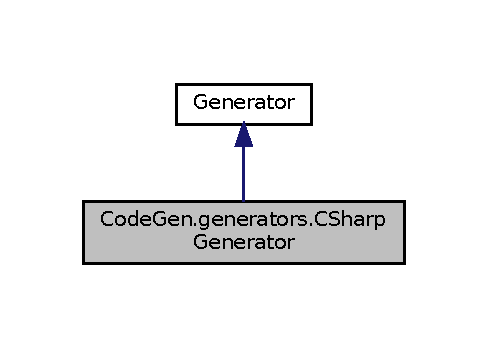
\includegraphics[width=234pt]{classCodeGen_1_1generators_1_1CSharpGenerator__inherit__graph}
\end{center}
\end{figure}


Collaboration diagram for Code\+Gen.\+generators.\+C\+Sharp\+Generator\+:
\nopagebreak
\begin{figure}[H]
\begin{center}
\leavevmode
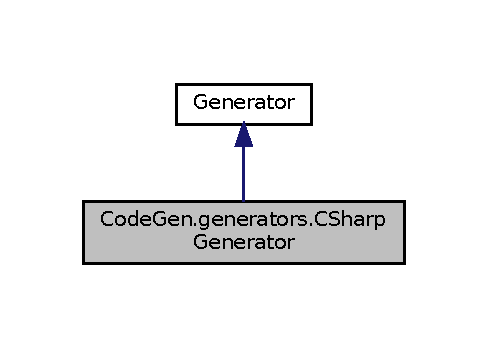
\includegraphics[width=234pt]{classCodeGen_1_1generators_1_1CSharpGenerator__coll__graph}
\end{center}
\end{figure}
\subsection*{Protected Member Functions}
\begin{DoxyCompactItemize}
\item 
override string \mbox{\hyperlink{classCodeGen_1_1generators_1_1CSharpGenerator_ae09fc218c8ddef8f13649ed278e93ff1}{Generate\+Class}} (\mbox{\hyperlink{classCodeGen_1_1generators_1_1Class}{Class}} @class)
\begin{DoxyCompactList}\small\item\em \mbox{\hyperlink{classCodeGen_1_1generators_1_1Class}{Class}} generator\+: generates class with fields, methods and subclasses from given class object  \end{DoxyCompactList}\item 
override string \mbox{\hyperlink{classCodeGen_1_1generators_1_1CSharpGenerator_a72ff9ea0d6e5119e5a720eb54a952201}{Generate\+Field}} (\mbox{\hyperlink{classCodeGen_1_1generators_1_1Field}{Field}} field)
\begin{DoxyCompactList}\small\item\em \mbox{\hyperlink{classCodeGen_1_1generators_1_1Field}{Field}} generator\+: generates field from given field object  \end{DoxyCompactList}\item 
override string \mbox{\hyperlink{classCodeGen_1_1generators_1_1CSharpGenerator_af39766dfe9c70d55091f7b8812bf8399}{Generate\+Method}} (\mbox{\hyperlink{classCodeGen_1_1generators_1_1Method}{Method}} method)
\begin{DoxyCompactList}\small\item\em \mbox{\hyperlink{classCodeGen_1_1generators_1_1Method}{Method}} generator\+: generates method from given method object  \end{DoxyCompactList}\end{DoxyCompactItemize}
\subsection*{Additional Inherited Members}


\subsection{Detailed Description}
C\# language generator 



\subsection{Member Function Documentation}
\mbox{\Hypertarget{classCodeGen_1_1generators_1_1CSharpGenerator_ae09fc218c8ddef8f13649ed278e93ff1}\label{classCodeGen_1_1generators_1_1CSharpGenerator_ae09fc218c8ddef8f13649ed278e93ff1}} 
\index{Code\+Gen\+::generators\+::\+C\+Sharp\+Generator@{Code\+Gen\+::generators\+::\+C\+Sharp\+Generator}!Generate\+Class@{Generate\+Class}}
\index{Generate\+Class@{Generate\+Class}!Code\+Gen\+::generators\+::\+C\+Sharp\+Generator@{Code\+Gen\+::generators\+::\+C\+Sharp\+Generator}}
\subsubsection{\texorpdfstring{Generate\+Class()}{GenerateClass()}}
{\footnotesize\ttfamily override string Code\+Gen.\+generators.\+C\+Sharp\+Generator.\+Generate\+Class (\begin{DoxyParamCaption}\item[{\mbox{\hyperlink{classCodeGen_1_1generators_1_1Class}{Class}} @}]{class }\end{DoxyParamCaption})\hspace{0.3cm}{\ttfamily [inline]}, {\ttfamily [protected]}, {\ttfamily [virtual]}}



\mbox{\hyperlink{classCodeGen_1_1generators_1_1Class}{Class}} generator\+: generates class with fields, methods and subclasses from given class object  



Implements \mbox{\hyperlink{classCodeGen_1_1generators_1_1Generator_a8847fd8b6d408a0dfc087dcc1dc58340}{Code\+Gen.\+generators.\+Generator}}.

\mbox{\Hypertarget{classCodeGen_1_1generators_1_1CSharpGenerator_a72ff9ea0d6e5119e5a720eb54a952201}\label{classCodeGen_1_1generators_1_1CSharpGenerator_a72ff9ea0d6e5119e5a720eb54a952201}} 
\index{Code\+Gen\+::generators\+::\+C\+Sharp\+Generator@{Code\+Gen\+::generators\+::\+C\+Sharp\+Generator}!Generate\+Field@{Generate\+Field}}
\index{Generate\+Field@{Generate\+Field}!Code\+Gen\+::generators\+::\+C\+Sharp\+Generator@{Code\+Gen\+::generators\+::\+C\+Sharp\+Generator}}
\subsubsection{\texorpdfstring{Generate\+Field()}{GenerateField()}}
{\footnotesize\ttfamily override string Code\+Gen.\+generators.\+C\+Sharp\+Generator.\+Generate\+Field (\begin{DoxyParamCaption}\item[{\mbox{\hyperlink{classCodeGen_1_1generators_1_1Field}{Field}}}]{field }\end{DoxyParamCaption})\hspace{0.3cm}{\ttfamily [inline]}, {\ttfamily [protected]}, {\ttfamily [virtual]}}



\mbox{\hyperlink{classCodeGen_1_1generators_1_1Field}{Field}} generator\+: generates field from given field object  



Implements \mbox{\hyperlink{classCodeGen_1_1generators_1_1Generator_a0d1a48aedbca08c05af734a43739d1c3}{Code\+Gen.\+generators.\+Generator}}.

\mbox{\Hypertarget{classCodeGen_1_1generators_1_1CSharpGenerator_af39766dfe9c70d55091f7b8812bf8399}\label{classCodeGen_1_1generators_1_1CSharpGenerator_af39766dfe9c70d55091f7b8812bf8399}} 
\index{Code\+Gen\+::generators\+::\+C\+Sharp\+Generator@{Code\+Gen\+::generators\+::\+C\+Sharp\+Generator}!Generate\+Method@{Generate\+Method}}
\index{Generate\+Method@{Generate\+Method}!Code\+Gen\+::generators\+::\+C\+Sharp\+Generator@{Code\+Gen\+::generators\+::\+C\+Sharp\+Generator}}
\subsubsection{\texorpdfstring{Generate\+Method()}{GenerateMethod()}}
{\footnotesize\ttfamily override string Code\+Gen.\+generators.\+C\+Sharp\+Generator.\+Generate\+Method (\begin{DoxyParamCaption}\item[{\mbox{\hyperlink{classCodeGen_1_1generators_1_1Method}{Method}}}]{method }\end{DoxyParamCaption})\hspace{0.3cm}{\ttfamily [inline]}, {\ttfamily [protected]}, {\ttfamily [virtual]}}



\mbox{\hyperlink{classCodeGen_1_1generators_1_1Method}{Method}} generator\+: generates method from given method object  



Implements \mbox{\hyperlink{classCodeGen_1_1generators_1_1Generator_a04fc9bd217b3b8c3d5f7b1a3f92c79d3}{Code\+Gen.\+generators.\+Generator}}.



The documentation for this class was generated from the following file\+:\begin{DoxyCompactItemize}
\item 
generators/\mbox{\hyperlink{CSharp_8cs}{C\+Sharp.\+cs}}\end{DoxyCompactItemize}

\hypertarget{classCodeGen_1_1generators_1_1ES6Generator}{}\section{Code\+Gen.\+generators.\+E\+S6\+Generator Class Reference}
\label{classCodeGen_1_1generators_1_1ES6Generator}\index{Code\+Gen.\+generators.\+E\+S6\+Generator@{Code\+Gen.\+generators.\+E\+S6\+Generator}}


\mbox{\hyperlink{classCodeGen_1_1generators_1_1Generator}{Generator}} for Java\+Script E\+S6  




Inheritance diagram for Code\+Gen.\+generators.\+E\+S6\+Generator\+:
\nopagebreak
\begin{figure}[H]
\begin{center}
\leavevmode
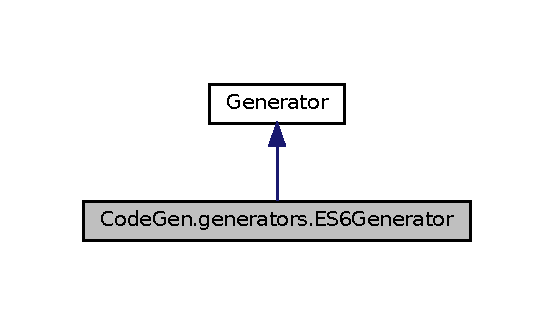
\includegraphics[width=266pt]{classCodeGen_1_1generators_1_1ES6Generator__inherit__graph}
\end{center}
\end{figure}


Collaboration diagram for Code\+Gen.\+generators.\+E\+S6\+Generator\+:
\nopagebreak
\begin{figure}[H]
\begin{center}
\leavevmode
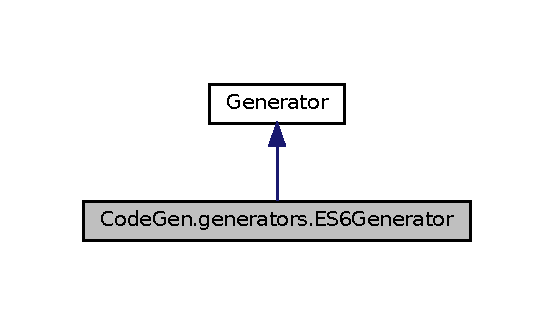
\includegraphics[width=266pt]{classCodeGen_1_1generators_1_1ES6Generator__coll__graph}
\end{center}
\end{figure}
\subsection*{Protected Member Functions}
\begin{DoxyCompactItemize}
\item 
override string \mbox{\hyperlink{classCodeGen_1_1generators_1_1ES6Generator_a53988e6898a5cf7b926e4c74a5af1703}{Generate\+Class}} (\mbox{\hyperlink{classCodeGen_1_1generators_1_1Class}{Class}} @class)
\begin{DoxyCompactList}\small\item\em \mbox{\hyperlink{classCodeGen_1_1generators_1_1Class}{Class}} generator\+: generates class with fields, methods and subclasses from given class object  \end{DoxyCompactList}\item 
override string \mbox{\hyperlink{classCodeGen_1_1generators_1_1ES6Generator_a35f257a51768270892dfa05dcf2c64c0}{Generate\+Field}} (\mbox{\hyperlink{classCodeGen_1_1generators_1_1Field}{Field}} field)
\begin{DoxyCompactList}\small\item\em \mbox{\hyperlink{classCodeGen_1_1generators_1_1Field}{Field}} generator\+: generates field from given field object  \end{DoxyCompactList}\item 
override string \mbox{\hyperlink{classCodeGen_1_1generators_1_1ES6Generator_a4107b28b436462ea13ce60b092c453f2}{Generate\+Method}} (\mbox{\hyperlink{classCodeGen_1_1generators_1_1Method}{Method}} method)
\begin{DoxyCompactList}\small\item\em \mbox{\hyperlink{classCodeGen_1_1generators_1_1Method}{Method}} generator\+: generates method from given method object  \end{DoxyCompactList}\end{DoxyCompactItemize}
\subsection*{Additional Inherited Members}


\subsection{Detailed Description}
\mbox{\hyperlink{classCodeGen_1_1generators_1_1Generator}{Generator}} for Java\+Script E\+S6 



\subsection{Member Function Documentation}
\mbox{\Hypertarget{classCodeGen_1_1generators_1_1ES6Generator_a53988e6898a5cf7b926e4c74a5af1703}\label{classCodeGen_1_1generators_1_1ES6Generator_a53988e6898a5cf7b926e4c74a5af1703}} 
\index{Code\+Gen\+::generators\+::\+E\+S6\+Generator@{Code\+Gen\+::generators\+::\+E\+S6\+Generator}!Generate\+Class@{Generate\+Class}}
\index{Generate\+Class@{Generate\+Class}!Code\+Gen\+::generators\+::\+E\+S6\+Generator@{Code\+Gen\+::generators\+::\+E\+S6\+Generator}}
\subsubsection{\texorpdfstring{Generate\+Class()}{GenerateClass()}}
{\footnotesize\ttfamily override string Code\+Gen.\+generators.\+E\+S6\+Generator.\+Generate\+Class (\begin{DoxyParamCaption}\item[{\mbox{\hyperlink{classCodeGen_1_1generators_1_1Class}{Class}} @}]{class }\end{DoxyParamCaption})\hspace{0.3cm}{\ttfamily [inline]}, {\ttfamily [protected]}, {\ttfamily [virtual]}}



\mbox{\hyperlink{classCodeGen_1_1generators_1_1Class}{Class}} generator\+: generates class with fields, methods and subclasses from given class object  



Implements \mbox{\hyperlink{classCodeGen_1_1generators_1_1Generator_a8847fd8b6d408a0dfc087dcc1dc58340}{Code\+Gen.\+generators.\+Generator}}.

\mbox{\Hypertarget{classCodeGen_1_1generators_1_1ES6Generator_a35f257a51768270892dfa05dcf2c64c0}\label{classCodeGen_1_1generators_1_1ES6Generator_a35f257a51768270892dfa05dcf2c64c0}} 
\index{Code\+Gen\+::generators\+::\+E\+S6\+Generator@{Code\+Gen\+::generators\+::\+E\+S6\+Generator}!Generate\+Field@{Generate\+Field}}
\index{Generate\+Field@{Generate\+Field}!Code\+Gen\+::generators\+::\+E\+S6\+Generator@{Code\+Gen\+::generators\+::\+E\+S6\+Generator}}
\subsubsection{\texorpdfstring{Generate\+Field()}{GenerateField()}}
{\footnotesize\ttfamily override string Code\+Gen.\+generators.\+E\+S6\+Generator.\+Generate\+Field (\begin{DoxyParamCaption}\item[{\mbox{\hyperlink{classCodeGen_1_1generators_1_1Field}{Field}}}]{field }\end{DoxyParamCaption})\hspace{0.3cm}{\ttfamily [inline]}, {\ttfamily [protected]}, {\ttfamily [virtual]}}



\mbox{\hyperlink{classCodeGen_1_1generators_1_1Field}{Field}} generator\+: generates field from given field object  



Implements \mbox{\hyperlink{classCodeGen_1_1generators_1_1Generator_a0d1a48aedbca08c05af734a43739d1c3}{Code\+Gen.\+generators.\+Generator}}.

\mbox{\Hypertarget{classCodeGen_1_1generators_1_1ES6Generator_a4107b28b436462ea13ce60b092c453f2}\label{classCodeGen_1_1generators_1_1ES6Generator_a4107b28b436462ea13ce60b092c453f2}} 
\index{Code\+Gen\+::generators\+::\+E\+S6\+Generator@{Code\+Gen\+::generators\+::\+E\+S6\+Generator}!Generate\+Method@{Generate\+Method}}
\index{Generate\+Method@{Generate\+Method}!Code\+Gen\+::generators\+::\+E\+S6\+Generator@{Code\+Gen\+::generators\+::\+E\+S6\+Generator}}
\subsubsection{\texorpdfstring{Generate\+Method()}{GenerateMethod()}}
{\footnotesize\ttfamily override string Code\+Gen.\+generators.\+E\+S6\+Generator.\+Generate\+Method (\begin{DoxyParamCaption}\item[{\mbox{\hyperlink{classCodeGen_1_1generators_1_1Method}{Method}}}]{method }\end{DoxyParamCaption})\hspace{0.3cm}{\ttfamily [inline]}, {\ttfamily [protected]}, {\ttfamily [virtual]}}



\mbox{\hyperlink{classCodeGen_1_1generators_1_1Method}{Method}} generator\+: generates method from given method object  



Implements \mbox{\hyperlink{classCodeGen_1_1generators_1_1Generator_a04fc9bd217b3b8c3d5f7b1a3f92c79d3}{Code\+Gen.\+generators.\+Generator}}.



The documentation for this class was generated from the following file\+:\begin{DoxyCompactItemize}
\item 
generators/\mbox{\hyperlink{ES6_8cs}{E\+S6.\+cs}}\end{DoxyCompactItemize}

\hypertarget{classCodeGen_1_1generators_1_1Field}{}\section{Code\+Gen.\+generators.\+Field Class Reference}
\label{classCodeGen_1_1generators_1_1Field}\index{Code\+Gen.\+generators.\+Field@{Code\+Gen.\+generators.\+Field}}


The structure that describes field. Contains access, const and static properties. Inherits from \mbox{\hyperlink{classCodeGen_1_1generators_1_1Variable}{Variable}}  




Inheritance diagram for Code\+Gen.\+generators.\+Field\+:
\nopagebreak
\begin{figure}[H]
\begin{center}
\leavevmode
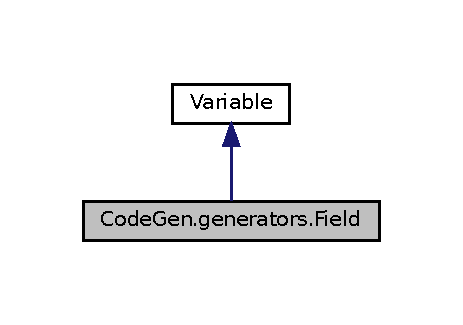
\includegraphics[width=222pt]{classCodeGen_1_1generators_1_1Field__inherit__graph}
\end{center}
\end{figure}


Collaboration diagram for Code\+Gen.\+generators.\+Field\+:
\nopagebreak
\begin{figure}[H]
\begin{center}
\leavevmode
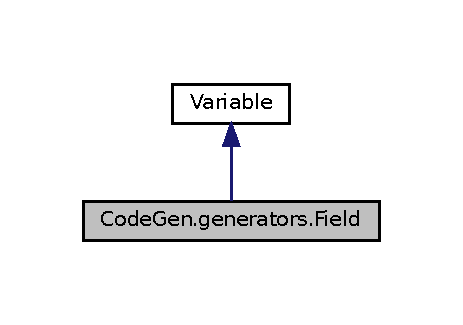
\includegraphics[width=222pt]{classCodeGen_1_1generators_1_1Field__coll__graph}
\end{center}
\end{figure}
\subsection*{Properties}
\begin{DoxyCompactItemize}
\item 
string \mbox{\hyperlink{classCodeGen_1_1generators_1_1Field_a49f206d40214424a35eefb0704371ad0}{Access}}\hspace{0.3cm}{\ttfamily  \mbox{[}get, set\mbox{]}}
\begin{DoxyCompactList}\small\item\em Represents access level of the field. Type\+: string \end{DoxyCompactList}\item 
bool \mbox{\hyperlink{classCodeGen_1_1generators_1_1Field_a13e03701c6d0b16e3ad7bdeda05a33aa}{Const}}\hspace{0.3cm}{\ttfamily  \mbox{[}get, set\mbox{]}}
\begin{DoxyCompactList}\small\item\em Denotes if field is constant or not. Type\+: boolean \end{DoxyCompactList}\item 
bool \mbox{\hyperlink{classCodeGen_1_1generators_1_1Field_a09f180833f4cf101aa0b4183407d7a80}{Static}}\hspace{0.3cm}{\ttfamily  \mbox{[}get, set\mbox{]}}
\begin{DoxyCompactList}\small\item\em Denotes if field is static or not. Type\+: boolean \end{DoxyCompactList}\item 
bool \mbox{\hyperlink{classCodeGen_1_1generators_1_1Field_aca6981cbfa9b6b370daef12a42e22662}{Getter}}\hspace{0.3cm}{\ttfamily  \mbox{[}get, set\mbox{]}}
\begin{DoxyCompactList}\small\item\em Denotes if generate getter or not. Type\+: boolean \end{DoxyCompactList}\item 
bool \mbox{\hyperlink{classCodeGen_1_1generators_1_1Field_ad57a32f584421475ceb3c929e56b20f9}{Setter}}\hspace{0.3cm}{\ttfamily  \mbox{[}get, set\mbox{]}}
\begin{DoxyCompactList}\small\item\em Denotes if generate setter or not. Type\+: boolean \end{DoxyCompactList}\end{DoxyCompactItemize}


\subsection{Detailed Description}
The structure that describes field. Contains access, const and static properties. Inherits from \mbox{\hyperlink{classCodeGen_1_1generators_1_1Variable}{Variable}} 



\subsection{Property Documentation}
\mbox{\Hypertarget{classCodeGen_1_1generators_1_1Field_a49f206d40214424a35eefb0704371ad0}\label{classCodeGen_1_1generators_1_1Field_a49f206d40214424a35eefb0704371ad0}} 
\index{Code\+Gen\+::generators\+::\+Field@{Code\+Gen\+::generators\+::\+Field}!Access@{Access}}
\index{Access@{Access}!Code\+Gen\+::generators\+::\+Field@{Code\+Gen\+::generators\+::\+Field}}
\subsubsection{\texorpdfstring{Access}{Access}}
{\footnotesize\ttfamily string Code\+Gen.\+generators.\+Field.\+Access\hspace{0.3cm}{\ttfamily [get]}, {\ttfamily [set]}}



Represents access level of the field. Type\+: string 

\mbox{\Hypertarget{classCodeGen_1_1generators_1_1Field_a13e03701c6d0b16e3ad7bdeda05a33aa}\label{classCodeGen_1_1generators_1_1Field_a13e03701c6d0b16e3ad7bdeda05a33aa}} 
\index{Code\+Gen\+::generators\+::\+Field@{Code\+Gen\+::generators\+::\+Field}!Const@{Const}}
\index{Const@{Const}!Code\+Gen\+::generators\+::\+Field@{Code\+Gen\+::generators\+::\+Field}}
\subsubsection{\texorpdfstring{Const}{Const}}
{\footnotesize\ttfamily bool Code\+Gen.\+generators.\+Field.\+Const\hspace{0.3cm}{\ttfamily [get]}, {\ttfamily [set]}}



Denotes if field is constant or not. Type\+: boolean 

\mbox{\Hypertarget{classCodeGen_1_1generators_1_1Field_aca6981cbfa9b6b370daef12a42e22662}\label{classCodeGen_1_1generators_1_1Field_aca6981cbfa9b6b370daef12a42e22662}} 
\index{Code\+Gen\+::generators\+::\+Field@{Code\+Gen\+::generators\+::\+Field}!Getter@{Getter}}
\index{Getter@{Getter}!Code\+Gen\+::generators\+::\+Field@{Code\+Gen\+::generators\+::\+Field}}
\subsubsection{\texorpdfstring{Getter}{Getter}}
{\footnotesize\ttfamily bool Code\+Gen.\+generators.\+Field.\+Getter\hspace{0.3cm}{\ttfamily [get]}, {\ttfamily [set]}}



Denotes if generate getter or not. Type\+: boolean 

\mbox{\Hypertarget{classCodeGen_1_1generators_1_1Field_ad57a32f584421475ceb3c929e56b20f9}\label{classCodeGen_1_1generators_1_1Field_ad57a32f584421475ceb3c929e56b20f9}} 
\index{Code\+Gen\+::generators\+::\+Field@{Code\+Gen\+::generators\+::\+Field}!Setter@{Setter}}
\index{Setter@{Setter}!Code\+Gen\+::generators\+::\+Field@{Code\+Gen\+::generators\+::\+Field}}
\subsubsection{\texorpdfstring{Setter}{Setter}}
{\footnotesize\ttfamily bool Code\+Gen.\+generators.\+Field.\+Setter\hspace{0.3cm}{\ttfamily [get]}, {\ttfamily [set]}}



Denotes if generate setter or not. Type\+: boolean 

\mbox{\Hypertarget{classCodeGen_1_1generators_1_1Field_a09f180833f4cf101aa0b4183407d7a80}\label{classCodeGen_1_1generators_1_1Field_a09f180833f4cf101aa0b4183407d7a80}} 
\index{Code\+Gen\+::generators\+::\+Field@{Code\+Gen\+::generators\+::\+Field}!Static@{Static}}
\index{Static@{Static}!Code\+Gen\+::generators\+::\+Field@{Code\+Gen\+::generators\+::\+Field}}
\subsubsection{\texorpdfstring{Static}{Static}}
{\footnotesize\ttfamily bool Code\+Gen.\+generators.\+Field.\+Static\hspace{0.3cm}{\ttfamily [get]}, {\ttfamily [set]}}



Denotes if field is static or not. Type\+: boolean 



The documentation for this class was generated from the following file\+:\begin{DoxyCompactItemize}
\item 
generators/\mbox{\hyperlink{Models_8cs}{Models.\+cs}}\end{DoxyCompactItemize}

\hypertarget{classCodeGen_1_1generators_1_1Generator}{}\section{Code\+Gen.\+generators.\+Generator Class Reference}
\label{classCodeGen_1_1generators_1_1Generator}\index{Code\+Gen.\+generators.\+Generator@{Code\+Gen.\+generators.\+Generator}}


Interface of language generator  




Inheritance diagram for Code\+Gen.\+generators.\+Generator\+:
\nopagebreak
\begin{figure}[H]
\begin{center}
\leavevmode
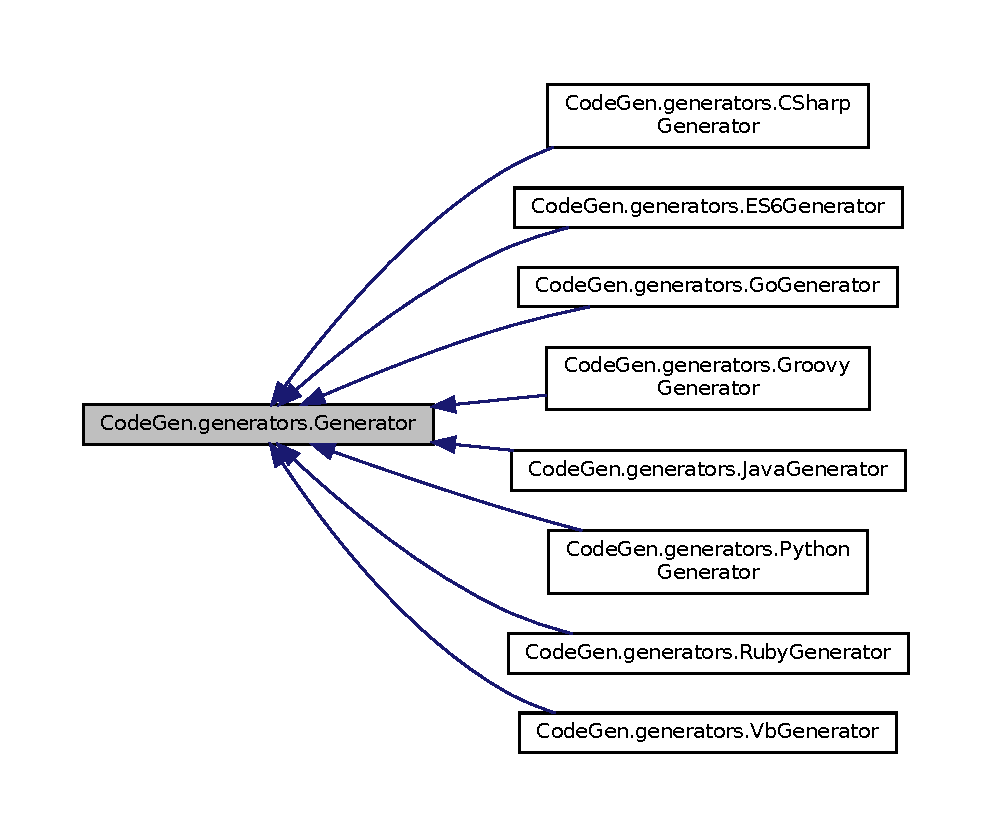
\includegraphics[width=350pt]{classCodeGen_1_1generators_1_1Generator__inherit__graph}
\end{center}
\end{figure}
\subsection*{Public Member Functions}
\begin{DoxyCompactItemize}
\item 
Dictionary$<$ string, string $>$ \mbox{\hyperlink{classCodeGen_1_1generators_1_1Generator_a5c5f7f56cdb910dc5d71ed407f874d84}{Generate}} (\mbox{\hyperlink{classCodeGen_1_1generators_1_1Package}{Package}} pkg)
\begin{DoxyCompactList}\small\item\em \mbox{\hyperlink{classCodeGen_1_1generators_1_1Package}{Package}} generator\+: generates package with classes and subpackages from given package object \end{DoxyCompactList}\end{DoxyCompactItemize}
\subsection*{Protected Member Functions}
\begin{DoxyCompactItemize}
\item 
abstract string \mbox{\hyperlink{classCodeGen_1_1generators_1_1Generator_a8847fd8b6d408a0dfc087dcc1dc58340}{Generate\+Class}} (\mbox{\hyperlink{classCodeGen_1_1generators_1_1Class}{Class}} @class)
\begin{DoxyCompactList}\small\item\em \mbox{\hyperlink{classCodeGen_1_1generators_1_1Class}{Class}} generator\+: generates class with fields, methods and subclasses from given class object \end{DoxyCompactList}\item 
abstract string \mbox{\hyperlink{classCodeGen_1_1generators_1_1Generator_a0d1a48aedbca08c05af734a43739d1c3}{Generate\+Field}} (\mbox{\hyperlink{classCodeGen_1_1generators_1_1Field}{Field}} field)
\begin{DoxyCompactList}\small\item\em \mbox{\hyperlink{classCodeGen_1_1generators_1_1Field}{Field}} generator\+: generates field from given field object \end{DoxyCompactList}\item 
abstract string \mbox{\hyperlink{classCodeGen_1_1generators_1_1Generator_a04fc9bd217b3b8c3d5f7b1a3f92c79d3}{Generate\+Method}} (\mbox{\hyperlink{classCodeGen_1_1generators_1_1Method}{Method}} method)
\begin{DoxyCompactList}\small\item\em \mbox{\hyperlink{classCodeGen_1_1generators_1_1Method}{Method}} generator\+: generates method from given method object \end{DoxyCompactList}\end{DoxyCompactItemize}
\subsection*{Static Protected Attributes}
\begin{DoxyCompactItemize}
\item 
static bool \mbox{\hyperlink{classCodeGen_1_1generators_1_1Generator_a7a3edb5addb8b879b39666718f32514d}{Use\+Tabs}} = true
\end{DoxyCompactItemize}


\subsection{Detailed Description}
Interface of language generator 



\subsection{Member Function Documentation}
\mbox{\Hypertarget{classCodeGen_1_1generators_1_1Generator_a5c5f7f56cdb910dc5d71ed407f874d84}\label{classCodeGen_1_1generators_1_1Generator_a5c5f7f56cdb910dc5d71ed407f874d84}} 
\index{Code\+Gen\+::generators\+::\+Generator@{Code\+Gen\+::generators\+::\+Generator}!Generate@{Generate}}
\index{Generate@{Generate}!Code\+Gen\+::generators\+::\+Generator@{Code\+Gen\+::generators\+::\+Generator}}
\subsubsection{\texorpdfstring{Generate()}{Generate()}}
{\footnotesize\ttfamily Dictionary$<$string, string$>$ Code\+Gen.\+generators.\+Generator.\+Generate (\begin{DoxyParamCaption}\item[{\mbox{\hyperlink{classCodeGen_1_1generators_1_1Package}{Package}}}]{pkg }\end{DoxyParamCaption})\hspace{0.3cm}{\ttfamily [inline]}}



\mbox{\hyperlink{classCodeGen_1_1generators_1_1Package}{Package}} generator\+: generates package with classes and subpackages from given package object 


\begin{DoxyParams}{Parameters}
{\em pkg} & \mbox{\hyperlink{classCodeGen_1_1generators_1_1Package}{Package}} object\\
\hline
\end{DoxyParams}
\begin{DoxyReturn}{Returns}
Dictionary of file names (keys) and generated code (values)
\end{DoxyReturn}
\mbox{\Hypertarget{classCodeGen_1_1generators_1_1Generator_a8847fd8b6d408a0dfc087dcc1dc58340}\label{classCodeGen_1_1generators_1_1Generator_a8847fd8b6d408a0dfc087dcc1dc58340}} 
\index{Code\+Gen\+::generators\+::\+Generator@{Code\+Gen\+::generators\+::\+Generator}!Generate\+Class@{Generate\+Class}}
\index{Generate\+Class@{Generate\+Class}!Code\+Gen\+::generators\+::\+Generator@{Code\+Gen\+::generators\+::\+Generator}}
\subsubsection{\texorpdfstring{Generate\+Class()}{GenerateClass()}}
{\footnotesize\ttfamily abstract string Code\+Gen.\+generators.\+Generator.\+Generate\+Class (\begin{DoxyParamCaption}\item[{\mbox{\hyperlink{classCodeGen_1_1generators_1_1Class}{Class}} @}]{class }\end{DoxyParamCaption})\hspace{0.3cm}{\ttfamily [protected]}, {\ttfamily [pure virtual]}}



\mbox{\hyperlink{classCodeGen_1_1generators_1_1Class}{Class}} generator\+: generates class with fields, methods and subclasses from given class object 


\begin{DoxyParams}{Parameters}
{\em class} & \mbox{\hyperlink{classCodeGen_1_1generators_1_1Class}{Class}} object\\
\hline
\end{DoxyParams}
\begin{DoxyReturn}{Returns}
String of generated code of class
\end{DoxyReturn}


Implemented in \mbox{\hyperlink{classCodeGen_1_1generators_1_1CSharpGenerator_ae09fc218c8ddef8f13649ed278e93ff1}{Code\+Gen.\+generators.\+C\+Sharp\+Generator}}, \mbox{\hyperlink{classCodeGen_1_1generators_1_1ES6Generator_a53988e6898a5cf7b926e4c74a5af1703}{Code\+Gen.\+generators.\+E\+S6\+Generator}}, \mbox{\hyperlink{classCodeGen_1_1generators_1_1PythonGenerator_a7ef1629fdf50856e1424ed4fd8be564c}{Code\+Gen.\+generators.\+Python\+Generator}}, \mbox{\hyperlink{classCodeGen_1_1generators_1_1RubyGenerator_a5d54d68890f2fc6c58e297f79647c033}{Code\+Gen.\+generators.\+Ruby\+Generator}}, \mbox{\hyperlink{classCodeGen_1_1generators_1_1VbGenerator_a78dd1bac9e915e214bb6a43b3ebc15b5}{Code\+Gen.\+generators.\+Vb\+Generator}}, \mbox{\hyperlink{classCodeGen_1_1generators_1_1GoGenerator_aacdb59f4942c999f06400f9f92732858}{Code\+Gen.\+generators.\+Go\+Generator}}, \mbox{\hyperlink{classCodeGen_1_1generators_1_1GroovyGenerator_af13381a7be697b1f22cbf39bc0ab0e8d}{Code\+Gen.\+generators.\+Groovy\+Generator}}, and \mbox{\hyperlink{classCodeGen_1_1generators_1_1JavaGenerator_aebc6618c4d20b03195d4dd2a9bd03ffb}{Code\+Gen.\+generators.\+Java\+Generator}}.

\mbox{\Hypertarget{classCodeGen_1_1generators_1_1Generator_a0d1a48aedbca08c05af734a43739d1c3}\label{classCodeGen_1_1generators_1_1Generator_a0d1a48aedbca08c05af734a43739d1c3}} 
\index{Code\+Gen\+::generators\+::\+Generator@{Code\+Gen\+::generators\+::\+Generator}!Generate\+Field@{Generate\+Field}}
\index{Generate\+Field@{Generate\+Field}!Code\+Gen\+::generators\+::\+Generator@{Code\+Gen\+::generators\+::\+Generator}}
\subsubsection{\texorpdfstring{Generate\+Field()}{GenerateField()}}
{\footnotesize\ttfamily abstract string Code\+Gen.\+generators.\+Generator.\+Generate\+Field (\begin{DoxyParamCaption}\item[{\mbox{\hyperlink{classCodeGen_1_1generators_1_1Field}{Field}}}]{field }\end{DoxyParamCaption})\hspace{0.3cm}{\ttfamily [protected]}, {\ttfamily [pure virtual]}}



\mbox{\hyperlink{classCodeGen_1_1generators_1_1Field}{Field}} generator\+: generates field from given field object 


\begin{DoxyParams}{Parameters}
{\em field} & \mbox{\hyperlink{classCodeGen_1_1generators_1_1Field}{Field}} object\\
\hline
\end{DoxyParams}
\begin{DoxyReturn}{Returns}
String of generated code of field
\end{DoxyReturn}


Implemented in \mbox{\hyperlink{classCodeGen_1_1generators_1_1CSharpGenerator_a72ff9ea0d6e5119e5a720eb54a952201}{Code\+Gen.\+generators.\+C\+Sharp\+Generator}}, \mbox{\hyperlink{classCodeGen_1_1generators_1_1ES6Generator_a35f257a51768270892dfa05dcf2c64c0}{Code\+Gen.\+generators.\+E\+S6\+Generator}}, \mbox{\hyperlink{classCodeGen_1_1generators_1_1PythonGenerator_aafd171ffd14980515eef644b929bd712}{Code\+Gen.\+generators.\+Python\+Generator}}, \mbox{\hyperlink{classCodeGen_1_1generators_1_1VbGenerator_a114f5fcd8cc13180701041b6d9815f3f}{Code\+Gen.\+generators.\+Vb\+Generator}}, \mbox{\hyperlink{classCodeGen_1_1generators_1_1GroovyGenerator_a8ccffd1ee31dfad7f7599ab0bca0dc6b}{Code\+Gen.\+generators.\+Groovy\+Generator}}, \mbox{\hyperlink{classCodeGen_1_1generators_1_1RubyGenerator_a08fbd6d88c129901aa159e3a9a706278}{Code\+Gen.\+generators.\+Ruby\+Generator}}, \mbox{\hyperlink{classCodeGen_1_1generators_1_1JavaGenerator_a84c05958d52e40e29a5a2157de4579e2}{Code\+Gen.\+generators.\+Java\+Generator}}, and \mbox{\hyperlink{classCodeGen_1_1generators_1_1GoGenerator_aa7417b36b964e679a37dfee960148768}{Code\+Gen.\+generators.\+Go\+Generator}}.

\mbox{\Hypertarget{classCodeGen_1_1generators_1_1Generator_a04fc9bd217b3b8c3d5f7b1a3f92c79d3}\label{classCodeGen_1_1generators_1_1Generator_a04fc9bd217b3b8c3d5f7b1a3f92c79d3}} 
\index{Code\+Gen\+::generators\+::\+Generator@{Code\+Gen\+::generators\+::\+Generator}!Generate\+Method@{Generate\+Method}}
\index{Generate\+Method@{Generate\+Method}!Code\+Gen\+::generators\+::\+Generator@{Code\+Gen\+::generators\+::\+Generator}}
\subsubsection{\texorpdfstring{Generate\+Method()}{GenerateMethod()}}
{\footnotesize\ttfamily abstract string Code\+Gen.\+generators.\+Generator.\+Generate\+Method (\begin{DoxyParamCaption}\item[{\mbox{\hyperlink{classCodeGen_1_1generators_1_1Method}{Method}}}]{method }\end{DoxyParamCaption})\hspace{0.3cm}{\ttfamily [protected]}, {\ttfamily [pure virtual]}}



\mbox{\hyperlink{classCodeGen_1_1generators_1_1Method}{Method}} generator\+: generates method from given method object 


\begin{DoxyParams}{Parameters}
{\em method} & \mbox{\hyperlink{classCodeGen_1_1generators_1_1Method}{Method}} object\\
\hline
\end{DoxyParams}
\begin{DoxyReturn}{Returns}
String of generated code of method
\end{DoxyReturn}


Implemented in \mbox{\hyperlink{classCodeGen_1_1generators_1_1CSharpGenerator_af39766dfe9c70d55091f7b8812bf8399}{Code\+Gen.\+generators.\+C\+Sharp\+Generator}}, \mbox{\hyperlink{classCodeGen_1_1generators_1_1JavaGenerator_a01dca6b9662f50fbd4735dbe97c99cc2}{Code\+Gen.\+generators.\+Java\+Generator}}, \mbox{\hyperlink{classCodeGen_1_1generators_1_1GroovyGenerator_a7c8d2446310971e10a24b802bd9c62a0}{Code\+Gen.\+generators.\+Groovy\+Generator}}, \mbox{\hyperlink{classCodeGen_1_1generators_1_1ES6Generator_a4107b28b436462ea13ce60b092c453f2}{Code\+Gen.\+generators.\+E\+S6\+Generator}}, \mbox{\hyperlink{classCodeGen_1_1generators_1_1PythonGenerator_a09ea61b8eb384efcc36aa3574f9cb6a8}{Code\+Gen.\+generators.\+Python\+Generator}}, \mbox{\hyperlink{classCodeGen_1_1generators_1_1RubyGenerator_aa37c187dae8e400b050dcddba10d216b}{Code\+Gen.\+generators.\+Ruby\+Generator}}, \mbox{\hyperlink{classCodeGen_1_1generators_1_1VbGenerator_ab8855feff4b8292c04a53362d270b34d}{Code\+Gen.\+generators.\+Vb\+Generator}}, and \mbox{\hyperlink{classCodeGen_1_1generators_1_1GoGenerator_ac732350d06454ed93f2053c0971c8fd9}{Code\+Gen.\+generators.\+Go\+Generator}}.



\subsection{Member Data Documentation}
\mbox{\Hypertarget{classCodeGen_1_1generators_1_1Generator_a7a3edb5addb8b879b39666718f32514d}\label{classCodeGen_1_1generators_1_1Generator_a7a3edb5addb8b879b39666718f32514d}} 
\index{Code\+Gen\+::generators\+::\+Generator@{Code\+Gen\+::generators\+::\+Generator}!Use\+Tabs@{Use\+Tabs}}
\index{Use\+Tabs@{Use\+Tabs}!Code\+Gen\+::generators\+::\+Generator@{Code\+Gen\+::generators\+::\+Generator}}
\subsubsection{\texorpdfstring{Use\+Tabs}{UseTabs}}
{\footnotesize\ttfamily bool Code\+Gen.\+generators.\+Generator.\+Use\+Tabs = true\hspace{0.3cm}{\ttfamily [static]}, {\ttfamily [protected]}}







The documentation for this class was generated from the following file\+:\begin{DoxyCompactItemize}
\item 
generators/\mbox{\hyperlink{GeneratorConf_8cs}{Generator\+Conf.\+cs}}\end{DoxyCompactItemize}

\hypertarget{classCodeGen_1_1generators_1_1GeneratorConf}{}\section{Code\+Gen.\+generators.\+Generator\+Conf Class Reference}
\label{classCodeGen_1_1generators_1_1GeneratorConf}\index{Code\+Gen.\+generators.\+Generator\+Conf@{Code\+Gen.\+generators.\+Generator\+Conf}}


Holds the configuration of generator  




Collaboration diagram for Code\+Gen.\+generators.\+Generator\+Conf\+:
\nopagebreak
\begin{figure}[H]
\begin{center}
\leavevmode
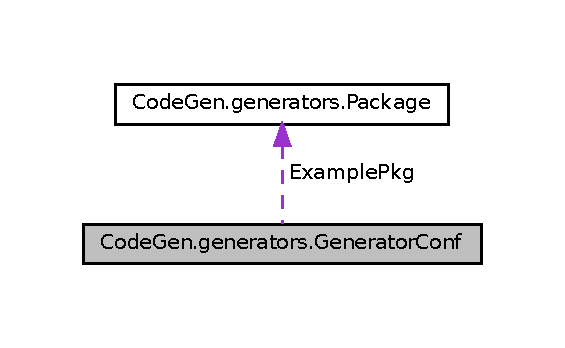
\includegraphics[width=271pt]{classCodeGen_1_1generators_1_1GeneratorConf__coll__graph}
\end{center}
\end{figure}
\subsection*{Static Public Member Functions}
\begin{DoxyCompactItemize}
\item 
static string \mbox{\hyperlink{classCodeGen_1_1generators_1_1GeneratorConf_a00082fad632c4dda77b1b025d1b2b280}{Get\+Indent}} (bool tabs, int tab\+Stop)
\begin{DoxyCompactList}\small\item\em Creates indent using given parameters \end{DoxyCompactList}\item 
static string \mbox{\hyperlink{classCodeGen_1_1generators_1_1GeneratorConf_a71dbec00a6e5d6d390dd8a24b64b6bb2}{Shift\+Code}} (string code, int num, string indent)
\begin{DoxyCompactList}\small\item\em Shifts code using given parameters \end{DoxyCompactList}\item 
static string \mbox{\hyperlink{classCodeGen_1_1generators_1_1GeneratorConf_a7b70aa3e67ba52dfbd1a271da20fc74e}{Normalize\+Lang}} (string lang)
\begin{DoxyCompactList}\small\item\em Converts given language into language which is used for identification of generator \end{DoxyCompactList}\item 
static \mbox{\hyperlink{structCodeGen_1_1generators_1_1Languange}{Languange}} \mbox{\hyperlink{classCodeGen_1_1generators_1_1GeneratorConf_a358bcc4be771d981ac1aa4c451b48383}{Get\+Language}} (string name)
\begin{DoxyCompactList}\small\item\em Creates generator if it exists, else throws an error \end{DoxyCompactList}\end{DoxyCompactItemize}
\subsection*{Static Public Attributes}
\begin{DoxyCompactItemize}
\item 
static readonly \mbox{\hyperlink{classCodeGen_1_1generators_1_1Package}{Package}} \mbox{\hyperlink{classCodeGen_1_1generators_1_1GeneratorConf_a9680e7722e2eb32214fa8ac1476f7903}{Example\+Pkg}}
\begin{DoxyCompactList}\small\item\em Contains example package \end{DoxyCompactList}\item 
static readonly Dictionary$<$ string, \mbox{\hyperlink{structCodeGen_1_1generators_1_1Languange}{Languange}} $>$ \mbox{\hyperlink{classCodeGen_1_1generators_1_1GeneratorConf_a830f7e81defcc68af267575792253b35}{Languanges}}
\begin{DoxyCompactList}\small\item\em Dictionary of language names (keys) and its Language objects (values) \end{DoxyCompactList}\end{DoxyCompactItemize}


\subsection{Detailed Description}
Holds the configuration of generator 



\subsection{Member Function Documentation}
\mbox{\Hypertarget{classCodeGen_1_1generators_1_1GeneratorConf_a00082fad632c4dda77b1b025d1b2b280}\label{classCodeGen_1_1generators_1_1GeneratorConf_a00082fad632c4dda77b1b025d1b2b280}} 
\index{Code\+Gen\+::generators\+::\+Generator\+Conf@{Code\+Gen\+::generators\+::\+Generator\+Conf}!Get\+Indent@{Get\+Indent}}
\index{Get\+Indent@{Get\+Indent}!Code\+Gen\+::generators\+::\+Generator\+Conf@{Code\+Gen\+::generators\+::\+Generator\+Conf}}
\subsubsection{\texorpdfstring{Get\+Indent()}{GetIndent()}}
{\footnotesize\ttfamily static string Code\+Gen.\+generators.\+Generator\+Conf.\+Get\+Indent (\begin{DoxyParamCaption}\item[{bool}]{tabs,  }\item[{int}]{tab\+Stop }\end{DoxyParamCaption})\hspace{0.3cm}{\ttfamily [inline]}, {\ttfamily [static]}}



Creates indent using given parameters 


\begin{DoxyParams}{Parameters}
{\em tabs} & Use tabs or spaces\\
\hline
{\em tab\+Stop} & Number of spaces\\
\hline
\end{DoxyParams}
\begin{DoxyReturn}{Returns}
Indent string
\end{DoxyReturn}
\mbox{\Hypertarget{classCodeGen_1_1generators_1_1GeneratorConf_a358bcc4be771d981ac1aa4c451b48383}\label{classCodeGen_1_1generators_1_1GeneratorConf_a358bcc4be771d981ac1aa4c451b48383}} 
\index{Code\+Gen\+::generators\+::\+Generator\+Conf@{Code\+Gen\+::generators\+::\+Generator\+Conf}!Get\+Language@{Get\+Language}}
\index{Get\+Language@{Get\+Language}!Code\+Gen\+::generators\+::\+Generator\+Conf@{Code\+Gen\+::generators\+::\+Generator\+Conf}}
\subsubsection{\texorpdfstring{Get\+Language()}{GetLanguage()}}
{\footnotesize\ttfamily static \mbox{\hyperlink{structCodeGen_1_1generators_1_1Languange}{Languange}} Code\+Gen.\+generators.\+Generator\+Conf.\+Get\+Language (\begin{DoxyParamCaption}\item[{string}]{name }\end{DoxyParamCaption})\hspace{0.3cm}{\ttfamily [inline]}, {\ttfamily [static]}}



Creates generator if it exists, else throws an error 


\begin{DoxyParams}{Parameters}
{\em name} & name of a language\\
\hline
\end{DoxyParams}
\begin{DoxyReturn}{Returns}
language
\end{DoxyReturn}

\begin{DoxyExceptions}{Exceptions}
{\em Index\+Out\+Of\+Range\+Exception} & If the language is not found\\
\hline
\end{DoxyExceptions}
\mbox{\Hypertarget{classCodeGen_1_1generators_1_1GeneratorConf_a7b70aa3e67ba52dfbd1a271da20fc74e}\label{classCodeGen_1_1generators_1_1GeneratorConf_a7b70aa3e67ba52dfbd1a271da20fc74e}} 
\index{Code\+Gen\+::generators\+::\+Generator\+Conf@{Code\+Gen\+::generators\+::\+Generator\+Conf}!Normalize\+Lang@{Normalize\+Lang}}
\index{Normalize\+Lang@{Normalize\+Lang}!Code\+Gen\+::generators\+::\+Generator\+Conf@{Code\+Gen\+::generators\+::\+Generator\+Conf}}
\subsubsection{\texorpdfstring{Normalize\+Lang()}{NormalizeLang()}}
{\footnotesize\ttfamily static string Code\+Gen.\+generators.\+Generator\+Conf.\+Normalize\+Lang (\begin{DoxyParamCaption}\item[{string}]{lang }\end{DoxyParamCaption})\hspace{0.3cm}{\ttfamily [inline]}, {\ttfamily [static]}}



Converts given language into language which is used for identification of generator 


\begin{DoxyParams}{Parameters}
{\em lang} & Inputed language\\
\hline
\end{DoxyParams}
\begin{DoxyReturn}{Returns}
Normalized language
\end{DoxyReturn}
\mbox{\Hypertarget{classCodeGen_1_1generators_1_1GeneratorConf_a71dbec00a6e5d6d390dd8a24b64b6bb2}\label{classCodeGen_1_1generators_1_1GeneratorConf_a71dbec00a6e5d6d390dd8a24b64b6bb2}} 
\index{Code\+Gen\+::generators\+::\+Generator\+Conf@{Code\+Gen\+::generators\+::\+Generator\+Conf}!Shift\+Code@{Shift\+Code}}
\index{Shift\+Code@{Shift\+Code}!Code\+Gen\+::generators\+::\+Generator\+Conf@{Code\+Gen\+::generators\+::\+Generator\+Conf}}
\subsubsection{\texorpdfstring{Shift\+Code()}{ShiftCode()}}
{\footnotesize\ttfamily static string Code\+Gen.\+generators.\+Generator\+Conf.\+Shift\+Code (\begin{DoxyParamCaption}\item[{string}]{code,  }\item[{int}]{num,  }\item[{string}]{indent }\end{DoxyParamCaption})\hspace{0.3cm}{\ttfamily [inline]}, {\ttfamily [static]}}



Shifts code using given parameters 


\begin{DoxyParams}{Parameters}
{\em code} & Code to be shifted\\
\hline
{\em num} & Number of indents\\
\hline
{\em indent} & Indent string\\
\hline
\end{DoxyParams}
\begin{DoxyReturn}{Returns}
Shifted code
\end{DoxyReturn}


\subsection{Member Data Documentation}
\mbox{\Hypertarget{classCodeGen_1_1generators_1_1GeneratorConf_a9680e7722e2eb32214fa8ac1476f7903}\label{classCodeGen_1_1generators_1_1GeneratorConf_a9680e7722e2eb32214fa8ac1476f7903}} 
\index{Code\+Gen\+::generators\+::\+Generator\+Conf@{Code\+Gen\+::generators\+::\+Generator\+Conf}!Example\+Pkg@{Example\+Pkg}}
\index{Example\+Pkg@{Example\+Pkg}!Code\+Gen\+::generators\+::\+Generator\+Conf@{Code\+Gen\+::generators\+::\+Generator\+Conf}}
\subsubsection{\texorpdfstring{Example\+Pkg}{ExamplePkg}}
{\footnotesize\ttfamily readonly \mbox{\hyperlink{classCodeGen_1_1generators_1_1Package}{Package}} Code\+Gen.\+generators.\+Generator\+Conf.\+Example\+Pkg\hspace{0.3cm}{\ttfamily [static]}}



Contains example package 

\mbox{\Hypertarget{classCodeGen_1_1generators_1_1GeneratorConf_a830f7e81defcc68af267575792253b35}\label{classCodeGen_1_1generators_1_1GeneratorConf_a830f7e81defcc68af267575792253b35}} 
\index{Code\+Gen\+::generators\+::\+Generator\+Conf@{Code\+Gen\+::generators\+::\+Generator\+Conf}!Languanges@{Languanges}}
\index{Languanges@{Languanges}!Code\+Gen\+::generators\+::\+Generator\+Conf@{Code\+Gen\+::generators\+::\+Generator\+Conf}}
\subsubsection{\texorpdfstring{Languanges}{Languanges}}
{\footnotesize\ttfamily readonly Dictionary$<$string, \mbox{\hyperlink{structCodeGen_1_1generators_1_1Languange}{Languange}}$>$ Code\+Gen.\+generators.\+Generator\+Conf.\+Languanges\hspace{0.3cm}{\ttfamily [static]}}

{\bfseries Initial value\+:}
\begin{DoxyCode}
= \textcolor{keyword}{new} Dictionary<string, Languange>
        \{
            \{\textcolor{stringliteral}{"java"}, \textcolor{keyword}{new} Languange(\textcolor{keyword}{new} JavaGenerator(), \textcolor{stringliteral}{"java"}, \textcolor{stringliteral}{"/* \{0\} */"})\},
            \{\textcolor{stringliteral}{"go"}, \textcolor{keyword}{new} Languange(\textcolor{keyword}{new} GoGenerator(), \textcolor{stringliteral}{"go"}, \textcolor{stringliteral}{"/* \{0\} */"})\},
            \{\textcolor{stringliteral}{"ruby"}, \textcolor{keyword}{new} Languange(\textcolor{keyword}{new} RubyGenerator(), \textcolor{stringliteral}{"rb"}, \textcolor{stringliteral}{"# \{0\}"})\},
            \{\textcolor{stringliteral}{"python"}, \textcolor{keyword}{new} Languange(\textcolor{keyword}{new} PythonGenerator(), \textcolor{stringliteral}{"py"}, \textcolor{stringliteral}{"# \{0\}\(\backslash\)n"})\},
            \{\textcolor{stringliteral}{"vb"}, \textcolor{keyword}{new} Languange(\textcolor{keyword}{new} VbGenerator(), \textcolor{stringliteral}{"vb"}, \textcolor{stringliteral}{"' \{0\}\(\backslash\)n"})\},
            \{\textcolor{stringliteral}{"csharp"}, \textcolor{keyword}{new} Languange(\textcolor{keyword}{new} CSharpGenerator(), \textcolor{stringliteral}{"cs"}, \textcolor{stringliteral}{"/* \{0\} */"})\},
            \{\textcolor{stringliteral}{"js\_es6"}, \textcolor{keyword}{new} Languange(\textcolor{keyword}{new} ES6Generator(), \textcolor{stringliteral}{"js"}, \textcolor{stringliteral}{"/* \{0\} */"})\},
            \{\textcolor{stringliteral}{"groovy"}, \textcolor{keyword}{new} Languange(\textcolor{keyword}{new} GroovyGenerator(), \textcolor{stringliteral}{"groovy"}, \textcolor{stringliteral}{"/* \{0\} */"})\},
            
            
        \}
\end{DoxyCode}


Dictionary of language names (keys) and its Language objects (values) 



The documentation for this class was generated from the following file\+:\begin{DoxyCompactItemize}
\item 
generators/\mbox{\hyperlink{GeneratorConf_8cs}{Generator\+Conf.\+cs}}\end{DoxyCompactItemize}

\hypertarget{classCodeGen_1_1tests_1_1generators_1_1GeneratorConfTest}{}\section{Code\+Gen.\+tests.\+generators.\+Generator\+Conf\+Test Class Reference}
\label{classCodeGen_1_1tests_1_1generators_1_1GeneratorConfTest}\index{Code\+Gen.\+tests.\+generators.\+Generator\+Conf\+Test@{Code\+Gen.\+tests.\+generators.\+Generator\+Conf\+Test}}


 


\subsection*{Public Member Functions}
\begin{DoxyCompactItemize}
\item 
void \mbox{\hyperlink{classCodeGen_1_1tests_1_1generators_1_1GeneratorConfTest_aa695d2d64351f9cfc01fa9a66cfcc5f0}{Get\+Indent\+Test}} ()
\item 
void \mbox{\hyperlink{classCodeGen_1_1tests_1_1generators_1_1GeneratorConfTest_a3a26863916eed6ddcc04a59873604f66}{Shift\+Code\+Test}} ()
\item 
void \mbox{\hyperlink{classCodeGen_1_1tests_1_1generators_1_1GeneratorConfTest_a20eae51f428fff499711262ea3f96e4d}{Normalize\+Lang\+Test}} ()
\item 
void \mbox{\hyperlink{classCodeGen_1_1tests_1_1generators_1_1GeneratorConfTest_a2b8c73a49a08299aee6cc08ba88ccdc9}{Get\+Language\+Test}} ()
\end{DoxyCompactItemize}


\subsection{Detailed Description}




\subsection{Member Function Documentation}
\mbox{\Hypertarget{classCodeGen_1_1tests_1_1generators_1_1GeneratorConfTest_aa695d2d64351f9cfc01fa9a66cfcc5f0}\label{classCodeGen_1_1tests_1_1generators_1_1GeneratorConfTest_aa695d2d64351f9cfc01fa9a66cfcc5f0}} 
\index{Code\+Gen\+::tests\+::generators\+::\+Generator\+Conf\+Test@{Code\+Gen\+::tests\+::generators\+::\+Generator\+Conf\+Test}!Get\+Indent\+Test@{Get\+Indent\+Test}}
\index{Get\+Indent\+Test@{Get\+Indent\+Test}!Code\+Gen\+::tests\+::generators\+::\+Generator\+Conf\+Test@{Code\+Gen\+::tests\+::generators\+::\+Generator\+Conf\+Test}}
\subsubsection{\texorpdfstring{Get\+Indent\+Test()}{GetIndentTest()}}
{\footnotesize\ttfamily void Code\+Gen.\+tests.\+generators.\+Generator\+Conf\+Test.\+Get\+Indent\+Test (\begin{DoxyParamCaption}{ }\end{DoxyParamCaption})\hspace{0.3cm}{\ttfamily [inline]}}





\mbox{\Hypertarget{classCodeGen_1_1tests_1_1generators_1_1GeneratorConfTest_a2b8c73a49a08299aee6cc08ba88ccdc9}\label{classCodeGen_1_1tests_1_1generators_1_1GeneratorConfTest_a2b8c73a49a08299aee6cc08ba88ccdc9}} 
\index{Code\+Gen\+::tests\+::generators\+::\+Generator\+Conf\+Test@{Code\+Gen\+::tests\+::generators\+::\+Generator\+Conf\+Test}!Get\+Language\+Test@{Get\+Language\+Test}}
\index{Get\+Language\+Test@{Get\+Language\+Test}!Code\+Gen\+::tests\+::generators\+::\+Generator\+Conf\+Test@{Code\+Gen\+::tests\+::generators\+::\+Generator\+Conf\+Test}}
\subsubsection{\texorpdfstring{Get\+Language\+Test()}{GetLanguageTest()}}
{\footnotesize\ttfamily void Code\+Gen.\+tests.\+generators.\+Generator\+Conf\+Test.\+Get\+Language\+Test (\begin{DoxyParamCaption}{ }\end{DoxyParamCaption})\hspace{0.3cm}{\ttfamily [inline]}}





\mbox{\Hypertarget{classCodeGen_1_1tests_1_1generators_1_1GeneratorConfTest_a20eae51f428fff499711262ea3f96e4d}\label{classCodeGen_1_1tests_1_1generators_1_1GeneratorConfTest_a20eae51f428fff499711262ea3f96e4d}} 
\index{Code\+Gen\+::tests\+::generators\+::\+Generator\+Conf\+Test@{Code\+Gen\+::tests\+::generators\+::\+Generator\+Conf\+Test}!Normalize\+Lang\+Test@{Normalize\+Lang\+Test}}
\index{Normalize\+Lang\+Test@{Normalize\+Lang\+Test}!Code\+Gen\+::tests\+::generators\+::\+Generator\+Conf\+Test@{Code\+Gen\+::tests\+::generators\+::\+Generator\+Conf\+Test}}
\subsubsection{\texorpdfstring{Normalize\+Lang\+Test()}{NormalizeLangTest()}}
{\footnotesize\ttfamily void Code\+Gen.\+tests.\+generators.\+Generator\+Conf\+Test.\+Normalize\+Lang\+Test (\begin{DoxyParamCaption}{ }\end{DoxyParamCaption})\hspace{0.3cm}{\ttfamily [inline]}}





\mbox{\Hypertarget{classCodeGen_1_1tests_1_1generators_1_1GeneratorConfTest_a3a26863916eed6ddcc04a59873604f66}\label{classCodeGen_1_1tests_1_1generators_1_1GeneratorConfTest_a3a26863916eed6ddcc04a59873604f66}} 
\index{Code\+Gen\+::tests\+::generators\+::\+Generator\+Conf\+Test@{Code\+Gen\+::tests\+::generators\+::\+Generator\+Conf\+Test}!Shift\+Code\+Test@{Shift\+Code\+Test}}
\index{Shift\+Code\+Test@{Shift\+Code\+Test}!Code\+Gen\+::tests\+::generators\+::\+Generator\+Conf\+Test@{Code\+Gen\+::tests\+::generators\+::\+Generator\+Conf\+Test}}
\subsubsection{\texorpdfstring{Shift\+Code\+Test()}{ShiftCodeTest()}}
{\footnotesize\ttfamily void Code\+Gen.\+tests.\+generators.\+Generator\+Conf\+Test.\+Shift\+Code\+Test (\begin{DoxyParamCaption}{ }\end{DoxyParamCaption})\hspace{0.3cm}{\ttfamily [inline]}}







The documentation for this class was generated from the following file\+:\begin{DoxyCompactItemize}
\item 
tests/generators/\mbox{\hyperlink{GeneratorConfTest_8cs}{Generator\+Conf\+Test.\+cs}}\end{DoxyCompactItemize}

\hypertarget{classCodeGen_1_1generators_1_1GoGenerator}{}\section{Code\+Gen.\+generators.\+Go\+Generator Class Reference}
\label{classCodeGen_1_1generators_1_1GoGenerator}\index{Code\+Gen.\+generators.\+Go\+Generator@{Code\+Gen.\+generators.\+Go\+Generator}}


Go language generator  




Inheritance diagram for Code\+Gen.\+generators.\+Go\+Generator\+:
\nopagebreak
\begin{figure}[H]
\begin{center}
\leavevmode
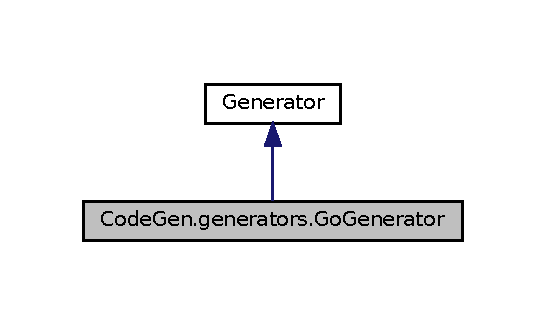
\includegraphics[width=262pt]{classCodeGen_1_1generators_1_1GoGenerator__inherit__graph}
\end{center}
\end{figure}


Collaboration diagram for Code\+Gen.\+generators.\+Go\+Generator\+:
\nopagebreak
\begin{figure}[H]
\begin{center}
\leavevmode
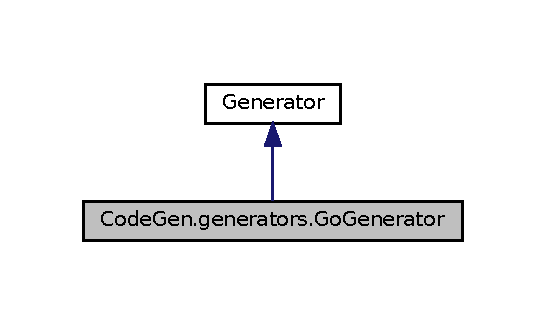
\includegraphics[width=262pt]{classCodeGen_1_1generators_1_1GoGenerator__coll__graph}
\end{center}
\end{figure}
\subsection*{Protected Member Functions}
\begin{DoxyCompactItemize}
\item 
override string \mbox{\hyperlink{classCodeGen_1_1generators_1_1GoGenerator_aacdb59f4942c999f06400f9f92732858}{Generate\+Class}} (\mbox{\hyperlink{classCodeGen_1_1generators_1_1Class}{Class}} @class)
\begin{DoxyCompactList}\small\item\em \mbox{\hyperlink{classCodeGen_1_1generators_1_1Class}{Class}} generator\+: generates class with fields, methods and subclasses from given class object  \end{DoxyCompactList}\item 
override string \mbox{\hyperlink{classCodeGen_1_1generators_1_1GoGenerator_aa7417b36b964e679a37dfee960148768}{Generate\+Field}} (\mbox{\hyperlink{classCodeGen_1_1generators_1_1Field}{Field}} field)
\begin{DoxyCompactList}\small\item\em \mbox{\hyperlink{classCodeGen_1_1generators_1_1Field}{Field}} generator\+: generates field from given field object  \end{DoxyCompactList}\item 
override string \mbox{\hyperlink{classCodeGen_1_1generators_1_1GoGenerator_ac732350d06454ed93f2053c0971c8fd9}{Generate\+Method}} (\mbox{\hyperlink{classCodeGen_1_1generators_1_1Method}{Method}} method)
\begin{DoxyCompactList}\small\item\em \mbox{\hyperlink{classCodeGen_1_1generators_1_1Method}{Method}} generator\+: generates method from given method object  \end{DoxyCompactList}\end{DoxyCompactItemize}
\subsection*{Additional Inherited Members}


\subsection{Detailed Description}
Go language generator 



\subsection{Member Function Documentation}
\mbox{\Hypertarget{classCodeGen_1_1generators_1_1GoGenerator_aacdb59f4942c999f06400f9f92732858}\label{classCodeGen_1_1generators_1_1GoGenerator_aacdb59f4942c999f06400f9f92732858}} 
\index{Code\+Gen\+::generators\+::\+Go\+Generator@{Code\+Gen\+::generators\+::\+Go\+Generator}!Generate\+Class@{Generate\+Class}}
\index{Generate\+Class@{Generate\+Class}!Code\+Gen\+::generators\+::\+Go\+Generator@{Code\+Gen\+::generators\+::\+Go\+Generator}}
\subsubsection{\texorpdfstring{Generate\+Class()}{GenerateClass()}}
{\footnotesize\ttfamily override string Code\+Gen.\+generators.\+Go\+Generator.\+Generate\+Class (\begin{DoxyParamCaption}\item[{\mbox{\hyperlink{classCodeGen_1_1generators_1_1Class}{Class}} @}]{class }\end{DoxyParamCaption})\hspace{0.3cm}{\ttfamily [inline]}, {\ttfamily [protected]}, {\ttfamily [virtual]}}



\mbox{\hyperlink{classCodeGen_1_1generators_1_1Class}{Class}} generator\+: generates class with fields, methods and subclasses from given class object  



Implements \mbox{\hyperlink{classCodeGen_1_1generators_1_1Generator_a8847fd8b6d408a0dfc087dcc1dc58340}{Code\+Gen.\+generators.\+Generator}}.

\mbox{\Hypertarget{classCodeGen_1_1generators_1_1GoGenerator_aa7417b36b964e679a37dfee960148768}\label{classCodeGen_1_1generators_1_1GoGenerator_aa7417b36b964e679a37dfee960148768}} 
\index{Code\+Gen\+::generators\+::\+Go\+Generator@{Code\+Gen\+::generators\+::\+Go\+Generator}!Generate\+Field@{Generate\+Field}}
\index{Generate\+Field@{Generate\+Field}!Code\+Gen\+::generators\+::\+Go\+Generator@{Code\+Gen\+::generators\+::\+Go\+Generator}}
\subsubsection{\texorpdfstring{Generate\+Field()}{GenerateField()}}
{\footnotesize\ttfamily override string Code\+Gen.\+generators.\+Go\+Generator.\+Generate\+Field (\begin{DoxyParamCaption}\item[{\mbox{\hyperlink{classCodeGen_1_1generators_1_1Field}{Field}}}]{field }\end{DoxyParamCaption})\hspace{0.3cm}{\ttfamily [inline]}, {\ttfamily [protected]}, {\ttfamily [virtual]}}



\mbox{\hyperlink{classCodeGen_1_1generators_1_1Field}{Field}} generator\+: generates field from given field object  



Implements \mbox{\hyperlink{classCodeGen_1_1generators_1_1Generator_a0d1a48aedbca08c05af734a43739d1c3}{Code\+Gen.\+generators.\+Generator}}.

\mbox{\Hypertarget{classCodeGen_1_1generators_1_1GoGenerator_ac732350d06454ed93f2053c0971c8fd9}\label{classCodeGen_1_1generators_1_1GoGenerator_ac732350d06454ed93f2053c0971c8fd9}} 
\index{Code\+Gen\+::generators\+::\+Go\+Generator@{Code\+Gen\+::generators\+::\+Go\+Generator}!Generate\+Method@{Generate\+Method}}
\index{Generate\+Method@{Generate\+Method}!Code\+Gen\+::generators\+::\+Go\+Generator@{Code\+Gen\+::generators\+::\+Go\+Generator}}
\subsubsection{\texorpdfstring{Generate\+Method()}{GenerateMethod()}}
{\footnotesize\ttfamily override string Code\+Gen.\+generators.\+Go\+Generator.\+Generate\+Method (\begin{DoxyParamCaption}\item[{\mbox{\hyperlink{classCodeGen_1_1generators_1_1Method}{Method}}}]{method }\end{DoxyParamCaption})\hspace{0.3cm}{\ttfamily [inline]}, {\ttfamily [protected]}, {\ttfamily [virtual]}}



\mbox{\hyperlink{classCodeGen_1_1generators_1_1Method}{Method}} generator\+: generates method from given method object  



Implements \mbox{\hyperlink{classCodeGen_1_1generators_1_1Generator_a04fc9bd217b3b8c3d5f7b1a3f92c79d3}{Code\+Gen.\+generators.\+Generator}}.



The documentation for this class was generated from the following file\+:\begin{DoxyCompactItemize}
\item 
generators/\mbox{\hyperlink{Go_8cs}{Go.\+cs}}\end{DoxyCompactItemize}

\hypertarget{classCodeGen_1_1generators_1_1GroovyGenerator}{}\section{Code\+Gen.\+generators.\+Groovy\+Generator Class Reference}
\label{classCodeGen_1_1generators_1_1GroovyGenerator}\index{Code\+Gen.\+generators.\+Groovy\+Generator@{Code\+Gen.\+generators.\+Groovy\+Generator}}


Groovy language generator  




Inheritance diagram for Code\+Gen.\+generators.\+Groovy\+Generator\+:
\nopagebreak
\begin{figure}[H]
\begin{center}
\leavevmode
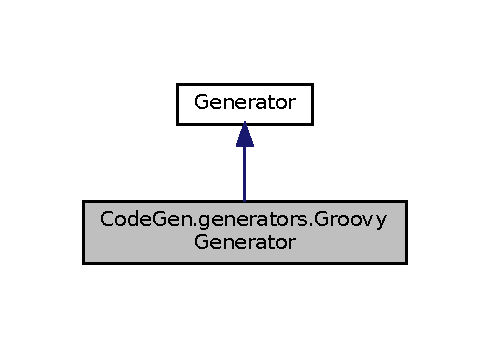
\includegraphics[width=235pt]{classCodeGen_1_1generators_1_1GroovyGenerator__inherit__graph}
\end{center}
\end{figure}


Collaboration diagram for Code\+Gen.\+generators.\+Groovy\+Generator\+:
\nopagebreak
\begin{figure}[H]
\begin{center}
\leavevmode
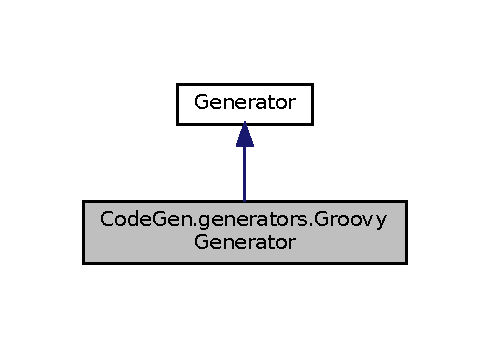
\includegraphics[width=235pt]{classCodeGen_1_1generators_1_1GroovyGenerator__coll__graph}
\end{center}
\end{figure}
\subsection*{Protected Member Functions}
\begin{DoxyCompactItemize}
\item 
override string \mbox{\hyperlink{classCodeGen_1_1generators_1_1GroovyGenerator_af13381a7be697b1f22cbf39bc0ab0e8d}{Generate\+Class}} (\mbox{\hyperlink{classCodeGen_1_1generators_1_1Class}{Class}} @class)
\begin{DoxyCompactList}\small\item\em \mbox{\hyperlink{classCodeGen_1_1generators_1_1Class}{Class}} generator\+: generates class with fields, methods and subclasses from given class object  \end{DoxyCompactList}\item 
override string \mbox{\hyperlink{classCodeGen_1_1generators_1_1GroovyGenerator_a8ccffd1ee31dfad7f7599ab0bca0dc6b}{Generate\+Field}} (\mbox{\hyperlink{classCodeGen_1_1generators_1_1Field}{Field}} field)
\begin{DoxyCompactList}\small\item\em \mbox{\hyperlink{classCodeGen_1_1generators_1_1Field}{Field}} generator\+: generates field from given field object  \end{DoxyCompactList}\item 
override string \mbox{\hyperlink{classCodeGen_1_1generators_1_1GroovyGenerator_a7c8d2446310971e10a24b802bd9c62a0}{Generate\+Method}} (\mbox{\hyperlink{classCodeGen_1_1generators_1_1Method}{Method}} method)
\begin{DoxyCompactList}\small\item\em \mbox{\hyperlink{classCodeGen_1_1generators_1_1Method}{Method}} generator\+: generates method from given method object  \end{DoxyCompactList}\end{DoxyCompactItemize}
\subsection*{Additional Inherited Members}


\subsection{Detailed Description}
Groovy language generator 



\subsection{Member Function Documentation}
\mbox{\Hypertarget{classCodeGen_1_1generators_1_1GroovyGenerator_af13381a7be697b1f22cbf39bc0ab0e8d}\label{classCodeGen_1_1generators_1_1GroovyGenerator_af13381a7be697b1f22cbf39bc0ab0e8d}} 
\index{Code\+Gen\+::generators\+::\+Groovy\+Generator@{Code\+Gen\+::generators\+::\+Groovy\+Generator}!Generate\+Class@{Generate\+Class}}
\index{Generate\+Class@{Generate\+Class}!Code\+Gen\+::generators\+::\+Groovy\+Generator@{Code\+Gen\+::generators\+::\+Groovy\+Generator}}
\subsubsection{\texorpdfstring{Generate\+Class()}{GenerateClass()}}
{\footnotesize\ttfamily override string Code\+Gen.\+generators.\+Groovy\+Generator.\+Generate\+Class (\begin{DoxyParamCaption}\item[{\mbox{\hyperlink{classCodeGen_1_1generators_1_1Class}{Class}} @}]{class }\end{DoxyParamCaption})\hspace{0.3cm}{\ttfamily [inline]}, {\ttfamily [protected]}, {\ttfamily [virtual]}}



\mbox{\hyperlink{classCodeGen_1_1generators_1_1Class}{Class}} generator\+: generates class with fields, methods and subclasses from given class object  



Implements \mbox{\hyperlink{classCodeGen_1_1generators_1_1Generator_a8847fd8b6d408a0dfc087dcc1dc58340}{Code\+Gen.\+generators.\+Generator}}.

\mbox{\Hypertarget{classCodeGen_1_1generators_1_1GroovyGenerator_a8ccffd1ee31dfad7f7599ab0bca0dc6b}\label{classCodeGen_1_1generators_1_1GroovyGenerator_a8ccffd1ee31dfad7f7599ab0bca0dc6b}} 
\index{Code\+Gen\+::generators\+::\+Groovy\+Generator@{Code\+Gen\+::generators\+::\+Groovy\+Generator}!Generate\+Field@{Generate\+Field}}
\index{Generate\+Field@{Generate\+Field}!Code\+Gen\+::generators\+::\+Groovy\+Generator@{Code\+Gen\+::generators\+::\+Groovy\+Generator}}
\subsubsection{\texorpdfstring{Generate\+Field()}{GenerateField()}}
{\footnotesize\ttfamily override string Code\+Gen.\+generators.\+Groovy\+Generator.\+Generate\+Field (\begin{DoxyParamCaption}\item[{\mbox{\hyperlink{classCodeGen_1_1generators_1_1Field}{Field}}}]{field }\end{DoxyParamCaption})\hspace{0.3cm}{\ttfamily [inline]}, {\ttfamily [protected]}, {\ttfamily [virtual]}}



\mbox{\hyperlink{classCodeGen_1_1generators_1_1Field}{Field}} generator\+: generates field from given field object  



Implements \mbox{\hyperlink{classCodeGen_1_1generators_1_1Generator_a0d1a48aedbca08c05af734a43739d1c3}{Code\+Gen.\+generators.\+Generator}}.

\mbox{\Hypertarget{classCodeGen_1_1generators_1_1GroovyGenerator_a7c8d2446310971e10a24b802bd9c62a0}\label{classCodeGen_1_1generators_1_1GroovyGenerator_a7c8d2446310971e10a24b802bd9c62a0}} 
\index{Code\+Gen\+::generators\+::\+Groovy\+Generator@{Code\+Gen\+::generators\+::\+Groovy\+Generator}!Generate\+Method@{Generate\+Method}}
\index{Generate\+Method@{Generate\+Method}!Code\+Gen\+::generators\+::\+Groovy\+Generator@{Code\+Gen\+::generators\+::\+Groovy\+Generator}}
\subsubsection{\texorpdfstring{Generate\+Method()}{GenerateMethod()}}
{\footnotesize\ttfamily override string Code\+Gen.\+generators.\+Groovy\+Generator.\+Generate\+Method (\begin{DoxyParamCaption}\item[{\mbox{\hyperlink{classCodeGen_1_1generators_1_1Method}{Method}}}]{method }\end{DoxyParamCaption})\hspace{0.3cm}{\ttfamily [inline]}, {\ttfamily [protected]}, {\ttfamily [virtual]}}



\mbox{\hyperlink{classCodeGen_1_1generators_1_1Method}{Method}} generator\+: generates method from given method object  



Implements \mbox{\hyperlink{classCodeGen_1_1generators_1_1Generator_a04fc9bd217b3b8c3d5f7b1a3f92c79d3}{Code\+Gen.\+generators.\+Generator}}.



The documentation for this class was generated from the following file\+:\begin{DoxyCompactItemize}
\item 
generators/\mbox{\hyperlink{Groovy_8cs}{Groovy.\+cs}}\end{DoxyCompactItemize}

\hypertarget{classCodeGen_1_1generators_1_1JavaGenerator}{}\section{Code\+Gen.\+generators.\+Java\+Generator Class Reference}
\label{classCodeGen_1_1generators_1_1JavaGenerator}\index{Code\+Gen.\+generators.\+Java\+Generator@{Code\+Gen.\+generators.\+Java\+Generator}}


Java language generator  




Inheritance diagram for Code\+Gen.\+generators.\+Java\+Generator\+:
\nopagebreak
\begin{figure}[H]
\begin{center}
\leavevmode
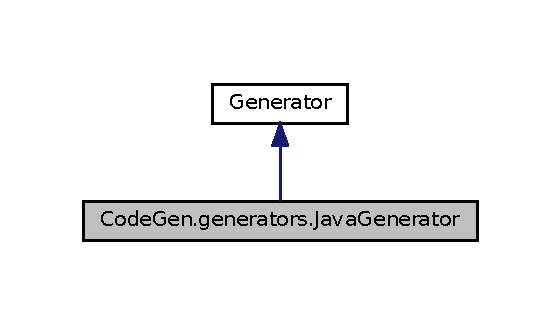
\includegraphics[width=269pt]{classCodeGen_1_1generators_1_1JavaGenerator__inherit__graph}
\end{center}
\end{figure}


Collaboration diagram for Code\+Gen.\+generators.\+Java\+Generator\+:
\nopagebreak
\begin{figure}[H]
\begin{center}
\leavevmode
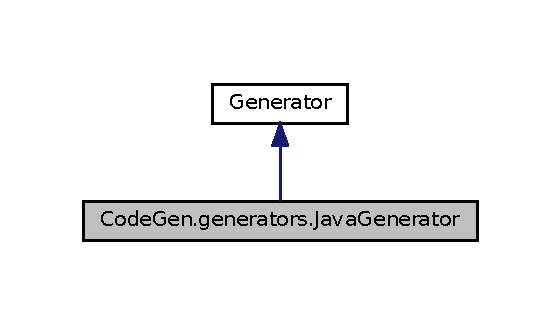
\includegraphics[width=269pt]{classCodeGen_1_1generators_1_1JavaGenerator__coll__graph}
\end{center}
\end{figure}
\subsection*{Protected Member Functions}
\begin{DoxyCompactItemize}
\item 
override string \mbox{\hyperlink{classCodeGen_1_1generators_1_1JavaGenerator_aebc6618c4d20b03195d4dd2a9bd03ffb}{Generate\+Class}} (\mbox{\hyperlink{classCodeGen_1_1generators_1_1Class}{Class}} @class)
\begin{DoxyCompactList}\small\item\em \mbox{\hyperlink{classCodeGen_1_1generators_1_1Class}{Class}} generator\+: generates class with fields, methods and subclasses from given class object  \end{DoxyCompactList}\item 
override string \mbox{\hyperlink{classCodeGen_1_1generators_1_1JavaGenerator_a84c05958d52e40e29a5a2157de4579e2}{Generate\+Field}} (\mbox{\hyperlink{classCodeGen_1_1generators_1_1Field}{Field}} field)
\begin{DoxyCompactList}\small\item\em \mbox{\hyperlink{classCodeGen_1_1generators_1_1Field}{Field}} generator\+: generates field from given field object  \end{DoxyCompactList}\item 
override string \mbox{\hyperlink{classCodeGen_1_1generators_1_1JavaGenerator_a01dca6b9662f50fbd4735dbe97c99cc2}{Generate\+Method}} (\mbox{\hyperlink{classCodeGen_1_1generators_1_1Method}{Method}} method)
\begin{DoxyCompactList}\small\item\em \mbox{\hyperlink{classCodeGen_1_1generators_1_1Method}{Method}} generator\+: generates method from given method object  \end{DoxyCompactList}\end{DoxyCompactItemize}
\subsection*{Additional Inherited Members}


\subsection{Detailed Description}
Java language generator 



\subsection{Member Function Documentation}
\mbox{\Hypertarget{classCodeGen_1_1generators_1_1JavaGenerator_aebc6618c4d20b03195d4dd2a9bd03ffb}\label{classCodeGen_1_1generators_1_1JavaGenerator_aebc6618c4d20b03195d4dd2a9bd03ffb}} 
\index{Code\+Gen\+::generators\+::\+Java\+Generator@{Code\+Gen\+::generators\+::\+Java\+Generator}!Generate\+Class@{Generate\+Class}}
\index{Generate\+Class@{Generate\+Class}!Code\+Gen\+::generators\+::\+Java\+Generator@{Code\+Gen\+::generators\+::\+Java\+Generator}}
\subsubsection{\texorpdfstring{Generate\+Class()}{GenerateClass()}}
{\footnotesize\ttfamily override string Code\+Gen.\+generators.\+Java\+Generator.\+Generate\+Class (\begin{DoxyParamCaption}\item[{\mbox{\hyperlink{classCodeGen_1_1generators_1_1Class}{Class}} @}]{class }\end{DoxyParamCaption})\hspace{0.3cm}{\ttfamily [inline]}, {\ttfamily [protected]}, {\ttfamily [virtual]}}



\mbox{\hyperlink{classCodeGen_1_1generators_1_1Class}{Class}} generator\+: generates class with fields, methods and subclasses from given class object  



Implements \mbox{\hyperlink{classCodeGen_1_1generators_1_1Generator_a8847fd8b6d408a0dfc087dcc1dc58340}{Code\+Gen.\+generators.\+Generator}}.

\mbox{\Hypertarget{classCodeGen_1_1generators_1_1JavaGenerator_a84c05958d52e40e29a5a2157de4579e2}\label{classCodeGen_1_1generators_1_1JavaGenerator_a84c05958d52e40e29a5a2157de4579e2}} 
\index{Code\+Gen\+::generators\+::\+Java\+Generator@{Code\+Gen\+::generators\+::\+Java\+Generator}!Generate\+Field@{Generate\+Field}}
\index{Generate\+Field@{Generate\+Field}!Code\+Gen\+::generators\+::\+Java\+Generator@{Code\+Gen\+::generators\+::\+Java\+Generator}}
\subsubsection{\texorpdfstring{Generate\+Field()}{GenerateField()}}
{\footnotesize\ttfamily override string Code\+Gen.\+generators.\+Java\+Generator.\+Generate\+Field (\begin{DoxyParamCaption}\item[{\mbox{\hyperlink{classCodeGen_1_1generators_1_1Field}{Field}}}]{field }\end{DoxyParamCaption})\hspace{0.3cm}{\ttfamily [inline]}, {\ttfamily [protected]}, {\ttfamily [virtual]}}



\mbox{\hyperlink{classCodeGen_1_1generators_1_1Field}{Field}} generator\+: generates field from given field object  



Implements \mbox{\hyperlink{classCodeGen_1_1generators_1_1Generator_a0d1a48aedbca08c05af734a43739d1c3}{Code\+Gen.\+generators.\+Generator}}.

\mbox{\Hypertarget{classCodeGen_1_1generators_1_1JavaGenerator_a01dca6b9662f50fbd4735dbe97c99cc2}\label{classCodeGen_1_1generators_1_1JavaGenerator_a01dca6b9662f50fbd4735dbe97c99cc2}} 
\index{Code\+Gen\+::generators\+::\+Java\+Generator@{Code\+Gen\+::generators\+::\+Java\+Generator}!Generate\+Method@{Generate\+Method}}
\index{Generate\+Method@{Generate\+Method}!Code\+Gen\+::generators\+::\+Java\+Generator@{Code\+Gen\+::generators\+::\+Java\+Generator}}
\subsubsection{\texorpdfstring{Generate\+Method()}{GenerateMethod()}}
{\footnotesize\ttfamily override string Code\+Gen.\+generators.\+Java\+Generator.\+Generate\+Method (\begin{DoxyParamCaption}\item[{\mbox{\hyperlink{classCodeGen_1_1generators_1_1Method}{Method}}}]{method }\end{DoxyParamCaption})\hspace{0.3cm}{\ttfamily [inline]}, {\ttfamily [protected]}, {\ttfamily [virtual]}}



\mbox{\hyperlink{classCodeGen_1_1generators_1_1Method}{Method}} generator\+: generates method from given method object  



Implements \mbox{\hyperlink{classCodeGen_1_1generators_1_1Generator_a04fc9bd217b3b8c3d5f7b1a3f92c79d3}{Code\+Gen.\+generators.\+Generator}}.



The documentation for this class was generated from the following file\+:\begin{DoxyCompactItemize}
\item 
generators/\mbox{\hyperlink{Java_8cs}{Java.\+cs}}\end{DoxyCompactItemize}

\hypertarget{structCodeGen_1_1generators_1_1Languange}{}\section{Code\+Gen.\+generators.\+Languange Struct Reference}
\label{structCodeGen_1_1generators_1_1Languange}\index{Code\+Gen.\+generators.\+Languange@{Code\+Gen.\+generators.\+Languange}}


The class that describes programming language and has a generator for it  




Collaboration diagram for Code\+Gen.\+generators.\+Languange\+:
\nopagebreak
\begin{figure}[H]
\begin{center}
\leavevmode
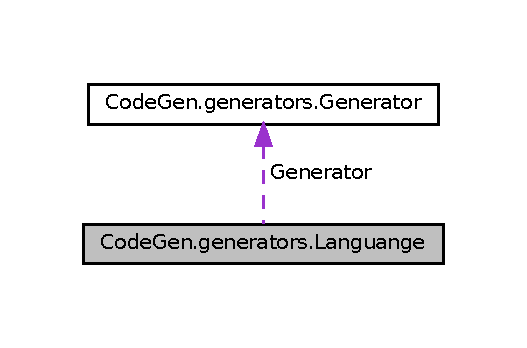
\includegraphics[width=253pt]{structCodeGen_1_1generators_1_1Languange__coll__graph}
\end{center}
\end{figure}
\subsection*{Public Member Functions}
\begin{DoxyCompactItemize}
\item 
\mbox{\hyperlink{structCodeGen_1_1generators_1_1Languange_a89fa98041473b18a7df845e14edcba07}{Languange}} (\mbox{\hyperlink{classCodeGen_1_1generators_1_1Generator}{Generator}} generator, string extension=\char`\"{}\char`\"{}, string comment=\char`\"{}\char`\"{}, \mbox{\hyperlink{classCodeGen_1_1generators_1_1Normalizer}{Normalizer}} normalizer=null, int indent\+Size=4)
\begin{DoxyCompactList}\small\item\em Constructor for language, used to avoid struct initializers \end{DoxyCompactList}\end{DoxyCompactItemize}
\subsection*{Public Attributes}
\begin{DoxyCompactItemize}
\item 
readonly \mbox{\hyperlink{classCodeGen_1_1generators_1_1Generator}{Generator}} \mbox{\hyperlink{structCodeGen_1_1generators_1_1Languange_a25fb0a47247497581d2d0560d0db66d8}{Generator}}
\begin{DoxyCompactList}\small\item\em Holds the generator of the language. \mbox{\hyperlink{classCodeGen_1_1generators_1_1Field}{Field}} is read only \end{DoxyCompactList}\item 
readonly string \mbox{\hyperlink{structCodeGen_1_1generators_1_1Languange_af00eae192536b05d637d0b81954202c7}{Extension}}
\begin{DoxyCompactList}\small\item\em Holds the extension of the file. \mbox{\hyperlink{classCodeGen_1_1generators_1_1Field}{Field}} is read only \end{DoxyCompactList}\item 
readonly string \mbox{\hyperlink{structCodeGen_1_1generators_1_1Languange_aa63aaf377bcac5ca06c14304701c3493}{Comment}}
\begin{DoxyCompactList}\small\item\em Holds comment format. \mbox{\hyperlink{classCodeGen_1_1generators_1_1Field}{Field}} is read only \end{DoxyCompactList}\item 
readonly int \mbox{\hyperlink{structCodeGen_1_1generators_1_1Languange_a3337b97358faf06c1e633e80f71cf2b4}{Indent\+Size}}
\begin{DoxyCompactList}\small\item\em The size of identation (works if using spaces, else 1 tab) \end{DoxyCompactList}\end{DoxyCompactItemize}


\subsection{Detailed Description}
The class that describes programming language and has a generator for it 



\subsection{Constructor \& Destructor Documentation}
\mbox{\Hypertarget{structCodeGen_1_1generators_1_1Languange_a89fa98041473b18a7df845e14edcba07}\label{structCodeGen_1_1generators_1_1Languange_a89fa98041473b18a7df845e14edcba07}} 
\index{Code\+Gen\+::generators\+::\+Languange@{Code\+Gen\+::generators\+::\+Languange}!Languange@{Languange}}
\index{Languange@{Languange}!Code\+Gen\+::generators\+::\+Languange@{Code\+Gen\+::generators\+::\+Languange}}
\subsubsection{\texorpdfstring{Languange()}{Languange()}}
{\footnotesize\ttfamily Code\+Gen.\+generators.\+Languange.\+Languange (\begin{DoxyParamCaption}\item[{\mbox{\hyperlink{classCodeGen_1_1generators_1_1Generator}{Generator}}}]{generator,  }\item[{string}]{extension = {\ttfamily \char`\"{}\char`\"{}},  }\item[{string}]{comment = {\ttfamily \char`\"{}\char`\"{}},  }\item[{\mbox{\hyperlink{classCodeGen_1_1generators_1_1Normalizer}{Normalizer}}}]{normalizer = {\ttfamily null},  }\item[{int}]{indent\+Size = {\ttfamily 4} }\end{DoxyParamCaption})\hspace{0.3cm}{\ttfamily [inline]}}



Constructor for language, used to avoid struct initializers 


\begin{DoxyParams}{Parameters}
{\em generator} & Language generator\\
\hline
{\em extension} & File extension\\
\hline
{\em comment} & Comment format\\
\hline
{\em normalizer} & Language normalizer\\
\hline
{\em indent\+Size} & The size of identation (works if using spaces, else 1 tab)\\
\hline
\end{DoxyParams}


\subsection{Member Data Documentation}
\mbox{\Hypertarget{structCodeGen_1_1generators_1_1Languange_aa63aaf377bcac5ca06c14304701c3493}\label{structCodeGen_1_1generators_1_1Languange_aa63aaf377bcac5ca06c14304701c3493}} 
\index{Code\+Gen\+::generators\+::\+Languange@{Code\+Gen\+::generators\+::\+Languange}!Comment@{Comment}}
\index{Comment@{Comment}!Code\+Gen\+::generators\+::\+Languange@{Code\+Gen\+::generators\+::\+Languange}}
\subsubsection{\texorpdfstring{Comment}{Comment}}
{\footnotesize\ttfamily readonly string Code\+Gen.\+generators.\+Languange.\+Comment}



Holds comment format. \mbox{\hyperlink{classCodeGen_1_1generators_1_1Field}{Field}} is read only 

\mbox{\Hypertarget{structCodeGen_1_1generators_1_1Languange_af00eae192536b05d637d0b81954202c7}\label{structCodeGen_1_1generators_1_1Languange_af00eae192536b05d637d0b81954202c7}} 
\index{Code\+Gen\+::generators\+::\+Languange@{Code\+Gen\+::generators\+::\+Languange}!Extension@{Extension}}
\index{Extension@{Extension}!Code\+Gen\+::generators\+::\+Languange@{Code\+Gen\+::generators\+::\+Languange}}
\subsubsection{\texorpdfstring{Extension}{Extension}}
{\footnotesize\ttfamily readonly string Code\+Gen.\+generators.\+Languange.\+Extension}



Holds the extension of the file. \mbox{\hyperlink{classCodeGen_1_1generators_1_1Field}{Field}} is read only 

\mbox{\Hypertarget{structCodeGen_1_1generators_1_1Languange_a25fb0a47247497581d2d0560d0db66d8}\label{structCodeGen_1_1generators_1_1Languange_a25fb0a47247497581d2d0560d0db66d8}} 
\index{Code\+Gen\+::generators\+::\+Languange@{Code\+Gen\+::generators\+::\+Languange}!Generator@{Generator}}
\index{Generator@{Generator}!Code\+Gen\+::generators\+::\+Languange@{Code\+Gen\+::generators\+::\+Languange}}
\subsubsection{\texorpdfstring{Generator}{Generator}}
{\footnotesize\ttfamily readonly \mbox{\hyperlink{classCodeGen_1_1generators_1_1Generator}{Generator}} Code\+Gen.\+generators.\+Languange.\+Generator}



Holds the generator of the language. \mbox{\hyperlink{classCodeGen_1_1generators_1_1Field}{Field}} is read only 

\mbox{\Hypertarget{structCodeGen_1_1generators_1_1Languange_a3337b97358faf06c1e633e80f71cf2b4}\label{structCodeGen_1_1generators_1_1Languange_a3337b97358faf06c1e633e80f71cf2b4}} 
\index{Code\+Gen\+::generators\+::\+Languange@{Code\+Gen\+::generators\+::\+Languange}!Indent\+Size@{Indent\+Size}}
\index{Indent\+Size@{Indent\+Size}!Code\+Gen\+::generators\+::\+Languange@{Code\+Gen\+::generators\+::\+Languange}}
\subsubsection{\texorpdfstring{Indent\+Size}{IndentSize}}
{\footnotesize\ttfamily readonly int Code\+Gen.\+generators.\+Languange.\+Indent\+Size}



The size of identation (works if using spaces, else 1 tab) 



The documentation for this struct was generated from the following file\+:\begin{DoxyCompactItemize}
\item 
generators/\mbox{\hyperlink{GeneratorConf_8cs}{Generator\+Conf.\+cs}}\end{DoxyCompactItemize}

\hypertarget{classCodeGen_1_1generators_1_1Method}{}\section{Code\+Gen.\+generators.\+Method Class Reference}
\label{classCodeGen_1_1generators_1_1Method}\index{Code\+Gen.\+generators.\+Method@{Code\+Gen.\+generators.\+Method}}


The structure that describes method. Contains name, return type, access level, const and static properties and array of parameters  


\subsection*{Properties}
\begin{DoxyCompactItemize}
\item 
string \mbox{\hyperlink{classCodeGen_1_1generators_1_1Method_a102f86b59635b173d66ed34541cf3e4c}{Name}}\hspace{0.3cm}{\ttfamily  \mbox{[}get, set\mbox{]}}
\begin{DoxyCompactList}\small\item\em Represents the name of the method. Type\+: string \end{DoxyCompactList}\item 
string \mbox{\hyperlink{classCodeGen_1_1generators_1_1Method_a1f14ec7aef5e61d595870f2fee56a885}{Return}}\hspace{0.3cm}{\ttfamily  \mbox{[}get, set\mbox{]}}
\begin{DoxyCompactList}\small\item\em Represents return type of the method. Type\+: string \end{DoxyCompactList}\item 
string \mbox{\hyperlink{classCodeGen_1_1generators_1_1Method_ad713380461315774e85e7316f9a48df9}{Access}}\hspace{0.3cm}{\ttfamily  \mbox{[}get, set\mbox{]}}
\begin{DoxyCompactList}\small\item\em Represents access level of the method. Type\+: string \end{DoxyCompactList}\item 
bool \mbox{\hyperlink{classCodeGen_1_1generators_1_1Method_a31ce28145fc93a8b16dc8a1132a73694}{Const}}\hspace{0.3cm}{\ttfamily  \mbox{[}get, set\mbox{]}}
\begin{DoxyCompactList}\small\item\em Denotes if the method is const or not. Type\+: boolean \end{DoxyCompactList}\item 
bool \mbox{\hyperlink{classCodeGen_1_1generators_1_1Method_a40aa2b9a7000ae6acc851b97410ce2af}{Static}}\hspace{0.3cm}{\ttfamily  \mbox{[}get, set\mbox{]}}
\begin{DoxyCompactList}\small\item\em Denotes if the mathod is static or not. Type\+: boolean \end{DoxyCompactList}\item 
\mbox{\hyperlink{classCodeGen_1_1generators_1_1Parameter}{Parameter}} \mbox{[}$\,$\mbox{]} \mbox{\hyperlink{classCodeGen_1_1generators_1_1Method_ae6898cecae4a670b5e72568bce89fea3}{Parameters}}\hspace{0.3cm}{\ttfamily  \mbox{[}get, set\mbox{]}}
\begin{DoxyCompactList}\small\item\em Represents parameters of the method. Type\+: array of type \mbox{\hyperlink{classCodeGen_1_1generators_1_1Parameter}{Parameter}} \end{DoxyCompactList}\end{DoxyCompactItemize}


\subsection{Detailed Description}
The structure that describes method. Contains name, return type, access level, const and static properties and array of parameters 



\subsection{Property Documentation}
\mbox{\Hypertarget{classCodeGen_1_1generators_1_1Method_ad713380461315774e85e7316f9a48df9}\label{classCodeGen_1_1generators_1_1Method_ad713380461315774e85e7316f9a48df9}} 
\index{Code\+Gen\+::generators\+::\+Method@{Code\+Gen\+::generators\+::\+Method}!Access@{Access}}
\index{Access@{Access}!Code\+Gen\+::generators\+::\+Method@{Code\+Gen\+::generators\+::\+Method}}
\subsubsection{\texorpdfstring{Access}{Access}}
{\footnotesize\ttfamily string Code\+Gen.\+generators.\+Method.\+Access\hspace{0.3cm}{\ttfamily [get]}, {\ttfamily [set]}}



Represents access level of the method. Type\+: string 

\mbox{\Hypertarget{classCodeGen_1_1generators_1_1Method_a31ce28145fc93a8b16dc8a1132a73694}\label{classCodeGen_1_1generators_1_1Method_a31ce28145fc93a8b16dc8a1132a73694}} 
\index{Code\+Gen\+::generators\+::\+Method@{Code\+Gen\+::generators\+::\+Method}!Const@{Const}}
\index{Const@{Const}!Code\+Gen\+::generators\+::\+Method@{Code\+Gen\+::generators\+::\+Method}}
\subsubsection{\texorpdfstring{Const}{Const}}
{\footnotesize\ttfamily bool Code\+Gen.\+generators.\+Method.\+Const\hspace{0.3cm}{\ttfamily [get]}, {\ttfamily [set]}}



Denotes if the method is const or not. Type\+: boolean 

\mbox{\Hypertarget{classCodeGen_1_1generators_1_1Method_a102f86b59635b173d66ed34541cf3e4c}\label{classCodeGen_1_1generators_1_1Method_a102f86b59635b173d66ed34541cf3e4c}} 
\index{Code\+Gen\+::generators\+::\+Method@{Code\+Gen\+::generators\+::\+Method}!Name@{Name}}
\index{Name@{Name}!Code\+Gen\+::generators\+::\+Method@{Code\+Gen\+::generators\+::\+Method}}
\subsubsection{\texorpdfstring{Name}{Name}}
{\footnotesize\ttfamily string Code\+Gen.\+generators.\+Method.\+Name\hspace{0.3cm}{\ttfamily [get]}, {\ttfamily [set]}}



Represents the name of the method. Type\+: string 

\mbox{\Hypertarget{classCodeGen_1_1generators_1_1Method_ae6898cecae4a670b5e72568bce89fea3}\label{classCodeGen_1_1generators_1_1Method_ae6898cecae4a670b5e72568bce89fea3}} 
\index{Code\+Gen\+::generators\+::\+Method@{Code\+Gen\+::generators\+::\+Method}!Parameters@{Parameters}}
\index{Parameters@{Parameters}!Code\+Gen\+::generators\+::\+Method@{Code\+Gen\+::generators\+::\+Method}}
\subsubsection{\texorpdfstring{Parameters}{Parameters}}
{\footnotesize\ttfamily \mbox{\hyperlink{classCodeGen_1_1generators_1_1Parameter}{Parameter}} \mbox{[}$\,$\mbox{]} Code\+Gen.\+generators.\+Method.\+Parameters\hspace{0.3cm}{\ttfamily [get]}, {\ttfamily [set]}}



Represents parameters of the method. Type\+: array of type \mbox{\hyperlink{classCodeGen_1_1generators_1_1Parameter}{Parameter}} 

\mbox{\Hypertarget{classCodeGen_1_1generators_1_1Method_a1f14ec7aef5e61d595870f2fee56a885}\label{classCodeGen_1_1generators_1_1Method_a1f14ec7aef5e61d595870f2fee56a885}} 
\index{Code\+Gen\+::generators\+::\+Method@{Code\+Gen\+::generators\+::\+Method}!Return@{Return}}
\index{Return@{Return}!Code\+Gen\+::generators\+::\+Method@{Code\+Gen\+::generators\+::\+Method}}
\subsubsection{\texorpdfstring{Return}{Return}}
{\footnotesize\ttfamily string Code\+Gen.\+generators.\+Method.\+Return\hspace{0.3cm}{\ttfamily [get]}, {\ttfamily [set]}}



Represents return type of the method. Type\+: string 

\mbox{\Hypertarget{classCodeGen_1_1generators_1_1Method_a40aa2b9a7000ae6acc851b97410ce2af}\label{classCodeGen_1_1generators_1_1Method_a40aa2b9a7000ae6acc851b97410ce2af}} 
\index{Code\+Gen\+::generators\+::\+Method@{Code\+Gen\+::generators\+::\+Method}!Static@{Static}}
\index{Static@{Static}!Code\+Gen\+::generators\+::\+Method@{Code\+Gen\+::generators\+::\+Method}}
\subsubsection{\texorpdfstring{Static}{Static}}
{\footnotesize\ttfamily bool Code\+Gen.\+generators.\+Method.\+Static\hspace{0.3cm}{\ttfamily [get]}, {\ttfamily [set]}}



Denotes if the mathod is static or not. Type\+: boolean 



The documentation for this class was generated from the following file\+:\begin{DoxyCompactItemize}
\item 
generators/\mbox{\hyperlink{Models_8cs}{Models.\+cs}}\end{DoxyCompactItemize}

\hypertarget{classCodeGen_1_1generators_1_1Normalizer}{}\section{Code\+Gen.\+generators.\+Normalizer Class Reference}
\label{classCodeGen_1_1generators_1_1Normalizer}\index{Code\+Gen.\+generators.\+Normalizer@{Code\+Gen.\+generators.\+Normalizer}}


Interface of language normalizer\+: normalizes package data according to specified language  




Inheritance diagram for Code\+Gen.\+generators.\+Normalizer\+:
\nopagebreak
\begin{figure}[H]
\begin{center}
\leavevmode
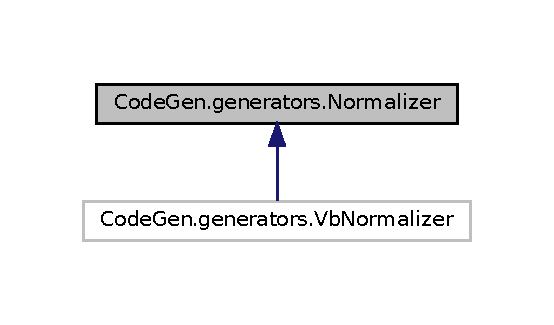
\includegraphics[width=266pt]{classCodeGen_1_1generators_1_1Normalizer__inherit__graph}
\end{center}
\end{figure}
\subsection*{Public Member Functions}
\begin{DoxyCompactItemize}
\item 
abstract \mbox{\hyperlink{classCodeGen_1_1generators_1_1Package}{Package}} \mbox{\hyperlink{classCodeGen_1_1generators_1_1Normalizer_a24212f04a2ed558c46ac62e23efcf0ae}{Normalize\+Package}} (\mbox{\hyperlink{classCodeGen_1_1generators_1_1Package}{Package}} pkg)
\begin{DoxyCompactList}\small\item\em \mbox{\hyperlink{classCodeGen_1_1generators_1_1Package}{Package}} normalizer\+: normalizes package with classes and subpackages \end{DoxyCompactList}\end{DoxyCompactItemize}
\subsection*{Protected Member Functions}
\begin{DoxyCompactItemize}
\item 
abstract \mbox{\hyperlink{classCodeGen_1_1generators_1_1Class}{Class}} \mbox{\hyperlink{classCodeGen_1_1generators_1_1Normalizer_ae79262a7509b9d78393262dccf63dcc5}{Normalize\+Class}} (\mbox{\hyperlink{classCodeGen_1_1generators_1_1Class}{Class}} @class)
\begin{DoxyCompactList}\small\item\em \mbox{\hyperlink{classCodeGen_1_1generators_1_1Class}{Class}} normalizer\+: normalizes class with fields, methods and subclasses \end{DoxyCompactList}\item 
abstract \mbox{\hyperlink{classCodeGen_1_1generators_1_1Field}{Field}} \mbox{\hyperlink{classCodeGen_1_1generators_1_1Normalizer_aafd7bd1d143fb2082a0e4ef53fcbb46b}{Normalize\+Field}} (\mbox{\hyperlink{classCodeGen_1_1generators_1_1Field}{Field}} field)
\begin{DoxyCompactList}\small\item\em \mbox{\hyperlink{classCodeGen_1_1generators_1_1Field}{Field}} normalizer\+: normalizes field \end{DoxyCompactList}\item 
abstract \mbox{\hyperlink{classCodeGen_1_1generators_1_1Method}{Method}} \mbox{\hyperlink{classCodeGen_1_1generators_1_1Normalizer_a68a4b1c8b53e9ce28507430412cb310e}{Normalize\+Method}} (\mbox{\hyperlink{classCodeGen_1_1generators_1_1Method}{Method}} method)
\begin{DoxyCompactList}\small\item\em \mbox{\hyperlink{classCodeGen_1_1generators_1_1Method}{Method}} normalizer\+: normalizes method \end{DoxyCompactList}\item 
abstract \mbox{\hyperlink{classCodeGen_1_1generators_1_1Parameter}{Parameter}} \mbox{\hyperlink{classCodeGen_1_1generators_1_1Normalizer_a981da1c9b6b487ba3043e538a4991000}{Normalize\+Parameter}} (\mbox{\hyperlink{classCodeGen_1_1generators_1_1Parameter}{Parameter}} parameter)
\begin{DoxyCompactList}\small\item\em \mbox{\hyperlink{classCodeGen_1_1generators_1_1Parameter}{Parameter}} normalizer\+: normalizes parameter \end{DoxyCompactList}\end{DoxyCompactItemize}


\subsection{Detailed Description}
Interface of language normalizer\+: normalizes package data according to specified language 



\subsection{Member Function Documentation}
\mbox{\Hypertarget{classCodeGen_1_1generators_1_1Normalizer_ae79262a7509b9d78393262dccf63dcc5}\label{classCodeGen_1_1generators_1_1Normalizer_ae79262a7509b9d78393262dccf63dcc5}} 
\index{Code\+Gen\+::generators\+::\+Normalizer@{Code\+Gen\+::generators\+::\+Normalizer}!Normalize\+Class@{Normalize\+Class}}
\index{Normalize\+Class@{Normalize\+Class}!Code\+Gen\+::generators\+::\+Normalizer@{Code\+Gen\+::generators\+::\+Normalizer}}
\subsubsection{\texorpdfstring{Normalize\+Class()}{NormalizeClass()}}
{\footnotesize\ttfamily abstract \mbox{\hyperlink{classCodeGen_1_1generators_1_1Class}{Class}} Code\+Gen.\+generators.\+Normalizer.\+Normalize\+Class (\begin{DoxyParamCaption}\item[{\mbox{\hyperlink{classCodeGen_1_1generators_1_1Class}{Class}} @}]{class }\end{DoxyParamCaption})\hspace{0.3cm}{\ttfamily [protected]}, {\ttfamily [pure virtual]}}



\mbox{\hyperlink{classCodeGen_1_1generators_1_1Class}{Class}} normalizer\+: normalizes class with fields, methods and subclasses 


\begin{DoxyParams}{Parameters}
{\em class} & \mbox{\hyperlink{classCodeGen_1_1generators_1_1Class}{Class}} object\\
\hline
\end{DoxyParams}
\begin{DoxyReturn}{Returns}
Normalized class object
\end{DoxyReturn}
\mbox{\Hypertarget{classCodeGen_1_1generators_1_1Normalizer_aafd7bd1d143fb2082a0e4ef53fcbb46b}\label{classCodeGen_1_1generators_1_1Normalizer_aafd7bd1d143fb2082a0e4ef53fcbb46b}} 
\index{Code\+Gen\+::generators\+::\+Normalizer@{Code\+Gen\+::generators\+::\+Normalizer}!Normalize\+Field@{Normalize\+Field}}
\index{Normalize\+Field@{Normalize\+Field}!Code\+Gen\+::generators\+::\+Normalizer@{Code\+Gen\+::generators\+::\+Normalizer}}
\subsubsection{\texorpdfstring{Normalize\+Field()}{NormalizeField()}}
{\footnotesize\ttfamily abstract \mbox{\hyperlink{classCodeGen_1_1generators_1_1Field}{Field}} Code\+Gen.\+generators.\+Normalizer.\+Normalize\+Field (\begin{DoxyParamCaption}\item[{\mbox{\hyperlink{classCodeGen_1_1generators_1_1Field}{Field}}}]{field }\end{DoxyParamCaption})\hspace{0.3cm}{\ttfamily [protected]}, {\ttfamily [pure virtual]}}



\mbox{\hyperlink{classCodeGen_1_1generators_1_1Field}{Field}} normalizer\+: normalizes field 


\begin{DoxyParams}{Parameters}
{\em field} & \mbox{\hyperlink{classCodeGen_1_1generators_1_1Field}{Field}} object\\
\hline
\end{DoxyParams}
\begin{DoxyReturn}{Returns}
Normalized field object
\end{DoxyReturn}
\mbox{\Hypertarget{classCodeGen_1_1generators_1_1Normalizer_a68a4b1c8b53e9ce28507430412cb310e}\label{classCodeGen_1_1generators_1_1Normalizer_a68a4b1c8b53e9ce28507430412cb310e}} 
\index{Code\+Gen\+::generators\+::\+Normalizer@{Code\+Gen\+::generators\+::\+Normalizer}!Normalize\+Method@{Normalize\+Method}}
\index{Normalize\+Method@{Normalize\+Method}!Code\+Gen\+::generators\+::\+Normalizer@{Code\+Gen\+::generators\+::\+Normalizer}}
\subsubsection{\texorpdfstring{Normalize\+Method()}{NormalizeMethod()}}
{\footnotesize\ttfamily abstract \mbox{\hyperlink{classCodeGen_1_1generators_1_1Method}{Method}} Code\+Gen.\+generators.\+Normalizer.\+Normalize\+Method (\begin{DoxyParamCaption}\item[{\mbox{\hyperlink{classCodeGen_1_1generators_1_1Method}{Method}}}]{method }\end{DoxyParamCaption})\hspace{0.3cm}{\ttfamily [protected]}, {\ttfamily [pure virtual]}}



\mbox{\hyperlink{classCodeGen_1_1generators_1_1Method}{Method}} normalizer\+: normalizes method 


\begin{DoxyParams}{Parameters}
{\em method} & \mbox{\hyperlink{classCodeGen_1_1generators_1_1Method}{Method}} object\\
\hline
\end{DoxyParams}
\begin{DoxyReturn}{Returns}
Normalized method object
\end{DoxyReturn}
\mbox{\Hypertarget{classCodeGen_1_1generators_1_1Normalizer_a24212f04a2ed558c46ac62e23efcf0ae}\label{classCodeGen_1_1generators_1_1Normalizer_a24212f04a2ed558c46ac62e23efcf0ae}} 
\index{Code\+Gen\+::generators\+::\+Normalizer@{Code\+Gen\+::generators\+::\+Normalizer}!Normalize\+Package@{Normalize\+Package}}
\index{Normalize\+Package@{Normalize\+Package}!Code\+Gen\+::generators\+::\+Normalizer@{Code\+Gen\+::generators\+::\+Normalizer}}
\subsubsection{\texorpdfstring{Normalize\+Package()}{NormalizePackage()}}
{\footnotesize\ttfamily abstract \mbox{\hyperlink{classCodeGen_1_1generators_1_1Package}{Package}} Code\+Gen.\+generators.\+Normalizer.\+Normalize\+Package (\begin{DoxyParamCaption}\item[{\mbox{\hyperlink{classCodeGen_1_1generators_1_1Package}{Package}}}]{pkg }\end{DoxyParamCaption})\hspace{0.3cm}{\ttfamily [pure virtual]}}



\mbox{\hyperlink{classCodeGen_1_1generators_1_1Package}{Package}} normalizer\+: normalizes package with classes and subpackages 


\begin{DoxyParams}{Parameters}
{\em pkg} & \mbox{\hyperlink{classCodeGen_1_1generators_1_1Package}{Package}} object\\
\hline
\end{DoxyParams}
\begin{DoxyReturn}{Returns}
Normalized package object
\end{DoxyReturn}
\mbox{\Hypertarget{classCodeGen_1_1generators_1_1Normalizer_a981da1c9b6b487ba3043e538a4991000}\label{classCodeGen_1_1generators_1_1Normalizer_a981da1c9b6b487ba3043e538a4991000}} 
\index{Code\+Gen\+::generators\+::\+Normalizer@{Code\+Gen\+::generators\+::\+Normalizer}!Normalize\+Parameter@{Normalize\+Parameter}}
\index{Normalize\+Parameter@{Normalize\+Parameter}!Code\+Gen\+::generators\+::\+Normalizer@{Code\+Gen\+::generators\+::\+Normalizer}}
\subsubsection{\texorpdfstring{Normalize\+Parameter()}{NormalizeParameter()}}
{\footnotesize\ttfamily abstract \mbox{\hyperlink{classCodeGen_1_1generators_1_1Parameter}{Parameter}} Code\+Gen.\+generators.\+Normalizer.\+Normalize\+Parameter (\begin{DoxyParamCaption}\item[{\mbox{\hyperlink{classCodeGen_1_1generators_1_1Parameter}{Parameter}}}]{parameter }\end{DoxyParamCaption})\hspace{0.3cm}{\ttfamily [protected]}, {\ttfamily [pure virtual]}}



\mbox{\hyperlink{classCodeGen_1_1generators_1_1Parameter}{Parameter}} normalizer\+: normalizes parameter 


\begin{DoxyParams}{Parameters}
{\em parameter} & \mbox{\hyperlink{classCodeGen_1_1generators_1_1Parameter}{Parameter}} object\\
\hline
\end{DoxyParams}
\begin{DoxyReturn}{Returns}
Normalized parameter object
\end{DoxyReturn}


The documentation for this class was generated from the following file\+:\begin{DoxyCompactItemize}
\item 
generators/\mbox{\hyperlink{GeneratorConf_8cs}{Generator\+Conf.\+cs}}\end{DoxyCompactItemize}

\hypertarget{classCodeGen_1_1generators_1_1Package}{}\section{Code\+Gen.\+generators.\+Package Class Reference}
\label{classCodeGen_1_1generators_1_1Package}\index{Code\+Gen.\+generators.\+Package@{Code\+Gen.\+generators.\+Package}}


The structure that describes package. Contains classes and subpackages  


\subsection*{Public Member Functions}
\begin{DoxyCompactItemize}
\item 
override string \mbox{\hyperlink{classCodeGen_1_1generators_1_1Package_a73029cd81fc68696bfe2d801ee382e69}{To\+String}} ()
\end{DoxyCompactItemize}
\subsection*{Properties}
\begin{DoxyCompactItemize}
\item 
string \mbox{\hyperlink{classCodeGen_1_1generators_1_1Package_a8da357302a6d399ce554f7a71bc4a90d}{Name}}\hspace{0.3cm}{\ttfamily  \mbox{[}get, set\mbox{]}}
\begin{DoxyCompactList}\small\item\em Represents the name of the package. Type\+: string \end{DoxyCompactList}\item 
bool \mbox{\hyperlink{classCodeGen_1_1generators_1_1Package_af03f90e7753d7fdc68699c32f86f82e9}{Use\+Spaces}}\hspace{0.3cm}{\ttfamily  \mbox{[}get, set\mbox{]}}
\begin{DoxyCompactList}\small\item\em Represents using of spaces or tabs. Type\+: boolean \end{DoxyCompactList}\item 
\mbox{\hyperlink{classCodeGen_1_1generators_1_1Class}{Class}} \mbox{[}$\,$\mbox{]} \mbox{\hyperlink{classCodeGen_1_1generators_1_1Package_a7bdaec0ad570345975582ca99076d4dd}{Classes}}\hspace{0.3cm}{\ttfamily  \mbox{[}get, set\mbox{]}}
\begin{DoxyCompactList}\small\item\em Represents classes. Type\+: array of type \mbox{\hyperlink{classCodeGen_1_1generators_1_1Class}{Class}} \end{DoxyCompactList}\item 
\mbox{\hyperlink{classCodeGen_1_1generators_1_1Package}{Package}} \mbox{[}$\,$\mbox{]} \mbox{\hyperlink{classCodeGen_1_1generators_1_1Package_a014a74cbc2bc2876e24d5a250cb54c68}{Packages}}\hspace{0.3cm}{\ttfamily  \mbox{[}get, set\mbox{]}}
\begin{DoxyCompactList}\small\item\em Represents subpackages. Type\+: array of type \mbox{\hyperlink{classCodeGen_1_1generators_1_1Package}{Package}} \end{DoxyCompactList}\end{DoxyCompactItemize}


\subsection{Detailed Description}
The structure that describes package. Contains classes and subpackages 



\subsection{Member Function Documentation}
\mbox{\Hypertarget{classCodeGen_1_1generators_1_1Package_a73029cd81fc68696bfe2d801ee382e69}\label{classCodeGen_1_1generators_1_1Package_a73029cd81fc68696bfe2d801ee382e69}} 
\index{Code\+Gen\+::generators\+::\+Package@{Code\+Gen\+::generators\+::\+Package}!To\+String@{To\+String}}
\index{To\+String@{To\+String}!Code\+Gen\+::generators\+::\+Package@{Code\+Gen\+::generators\+::\+Package}}
\subsubsection{\texorpdfstring{To\+String()}{ToString()}}
{\footnotesize\ttfamily override string Code\+Gen.\+generators.\+Package.\+To\+String (\begin{DoxyParamCaption}{ }\end{DoxyParamCaption})\hspace{0.3cm}{\ttfamily [inline]}}







\subsection{Property Documentation}
\mbox{\Hypertarget{classCodeGen_1_1generators_1_1Package_a7bdaec0ad570345975582ca99076d4dd}\label{classCodeGen_1_1generators_1_1Package_a7bdaec0ad570345975582ca99076d4dd}} 
\index{Code\+Gen\+::generators\+::\+Package@{Code\+Gen\+::generators\+::\+Package}!Classes@{Classes}}
\index{Classes@{Classes}!Code\+Gen\+::generators\+::\+Package@{Code\+Gen\+::generators\+::\+Package}}
\subsubsection{\texorpdfstring{Classes}{Classes}}
{\footnotesize\ttfamily \mbox{\hyperlink{classCodeGen_1_1generators_1_1Class}{Class}} \mbox{[}$\,$\mbox{]} Code\+Gen.\+generators.\+Package.\+Classes\hspace{0.3cm}{\ttfamily [get]}, {\ttfamily [set]}}



Represents classes. Type\+: array of type \mbox{\hyperlink{classCodeGen_1_1generators_1_1Class}{Class}} 

\mbox{\Hypertarget{classCodeGen_1_1generators_1_1Package_a8da357302a6d399ce554f7a71bc4a90d}\label{classCodeGen_1_1generators_1_1Package_a8da357302a6d399ce554f7a71bc4a90d}} 
\index{Code\+Gen\+::generators\+::\+Package@{Code\+Gen\+::generators\+::\+Package}!Name@{Name}}
\index{Name@{Name}!Code\+Gen\+::generators\+::\+Package@{Code\+Gen\+::generators\+::\+Package}}
\subsubsection{\texorpdfstring{Name}{Name}}
{\footnotesize\ttfamily string Code\+Gen.\+generators.\+Package.\+Name\hspace{0.3cm}{\ttfamily [get]}, {\ttfamily [set]}}



Represents the name of the package. Type\+: string 

\mbox{\Hypertarget{classCodeGen_1_1generators_1_1Package_a014a74cbc2bc2876e24d5a250cb54c68}\label{classCodeGen_1_1generators_1_1Package_a014a74cbc2bc2876e24d5a250cb54c68}} 
\index{Code\+Gen\+::generators\+::\+Package@{Code\+Gen\+::generators\+::\+Package}!Packages@{Packages}}
\index{Packages@{Packages}!Code\+Gen\+::generators\+::\+Package@{Code\+Gen\+::generators\+::\+Package}}
\subsubsection{\texorpdfstring{Packages}{Packages}}
{\footnotesize\ttfamily \mbox{\hyperlink{classCodeGen_1_1generators_1_1Package}{Package}} \mbox{[}$\,$\mbox{]} Code\+Gen.\+generators.\+Package.\+Packages\hspace{0.3cm}{\ttfamily [get]}, {\ttfamily [set]}}



Represents subpackages. Type\+: array of type \mbox{\hyperlink{classCodeGen_1_1generators_1_1Package}{Package}} 

\mbox{\Hypertarget{classCodeGen_1_1generators_1_1Package_af03f90e7753d7fdc68699c32f86f82e9}\label{classCodeGen_1_1generators_1_1Package_af03f90e7753d7fdc68699c32f86f82e9}} 
\index{Code\+Gen\+::generators\+::\+Package@{Code\+Gen\+::generators\+::\+Package}!Use\+Spaces@{Use\+Spaces}}
\index{Use\+Spaces@{Use\+Spaces}!Code\+Gen\+::generators\+::\+Package@{Code\+Gen\+::generators\+::\+Package}}
\subsubsection{\texorpdfstring{Use\+Spaces}{UseSpaces}}
{\footnotesize\ttfamily bool Code\+Gen.\+generators.\+Package.\+Use\+Spaces\hspace{0.3cm}{\ttfamily [get]}, {\ttfamily [set]}}



Represents using of spaces or tabs. Type\+: boolean 



The documentation for this class was generated from the following file\+:\begin{DoxyCompactItemize}
\item 
generators/\mbox{\hyperlink{Models_8cs}{Models.\+cs}}\end{DoxyCompactItemize}

\hypertarget{classCodeGen_1_1generators_1_1Parameter}{}\section{Code\+Gen.\+generators.\+Parameter Class Reference}
\label{classCodeGen_1_1generators_1_1Parameter}\index{Code\+Gen.\+generators.\+Parameter@{Code\+Gen.\+generators.\+Parameter}}


The structure that describes parameter. Inherits from \mbox{\hyperlink{classCodeGen_1_1generators_1_1Variable}{Variable}}  




Inheritance diagram for Code\+Gen.\+generators.\+Parameter\+:
\nopagebreak
\begin{figure}[H]
\begin{center}
\leavevmode
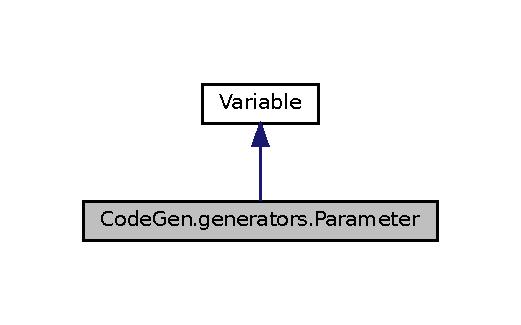
\includegraphics[width=250pt]{classCodeGen_1_1generators_1_1Parameter__inherit__graph}
\end{center}
\end{figure}


Collaboration diagram for Code\+Gen.\+generators.\+Parameter\+:
\nopagebreak
\begin{figure}[H]
\begin{center}
\leavevmode
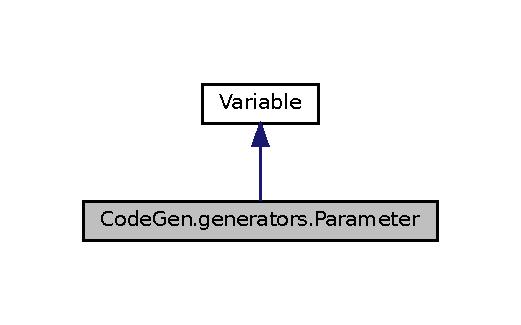
\includegraphics[width=250pt]{classCodeGen_1_1generators_1_1Parameter__coll__graph}
\end{center}
\end{figure}
\subsection*{Additional Inherited Members}


\subsection{Detailed Description}
The structure that describes parameter. Inherits from \mbox{\hyperlink{classCodeGen_1_1generators_1_1Variable}{Variable}} 



The documentation for this class was generated from the following file\+:\begin{DoxyCompactItemize}
\item 
generators/\mbox{\hyperlink{Models_8cs}{Models.\+cs}}\end{DoxyCompactItemize}

\hypertarget{classCodeGen_1_1parser_1_1Parser}{}\section{Code\+Gen.\+parser.\+Parser Class Reference}
\label{classCodeGen_1_1parser_1_1Parser}\index{Code\+Gen.\+parser.\+Parser@{Code\+Gen.\+parser.\+Parser}}


\mbox{\hyperlink{classCodeGen_1_1parser_1_1Parser}{Parser}}  


\subsection*{Static Public Member Functions}
\begin{DoxyCompactItemize}
\item 
static string \mbox{\hyperlink{classCodeGen_1_1parser_1_1Parser_af3a5d34f3773eff03e97c42b40ea3e96}{Read}} (string name)
\begin{DoxyCompactList}\small\item\em Reads file by file path \end{DoxyCompactList}\item 
static void \mbox{\hyperlink{classCodeGen_1_1parser_1_1Parser_a1d09a5fa154036958d654c65d3e64d7b}{Write}} (string path, string file\+Context)
\begin{DoxyCompactList}\small\item\em Writes string to a file \end{DoxyCompactList}\item 
static string \mbox{\hyperlink{classCodeGen_1_1parser_1_1Parser_aa8dc1a017c221d468885fd1ad7043de4}{Download}} (string url)
\begin{DoxyCompactList}\small\item\em Downloads file from the server by url \end{DoxyCompactList}\item 
static void \mbox{\hyperlink{classCodeGen_1_1parser_1_1Parser_addb0a8b1127eb9907303d4c09c2bf841}{Validate\+Args}} (string lang, string file, string url)
\begin{DoxyCompactList}\small\item\em Validates arguments given from command line \end{DoxyCompactList}\item 
static string \mbox{\hyperlink{classCodeGen_1_1parser_1_1Parser_a3297d7993fc6c739b3ff74f469c0589a}{Get\+File\+Format}} (string name)
\begin{DoxyCompactList}\small\item\em Gets file format by extension \end{DoxyCompactList}\item 
static string \mbox{\hyperlink{classCodeGen_1_1parser_1_1Parser_aaa59afdc45cfc1c9583c40e11791fc15}{Title}} (string @string)
\begin{DoxyCompactList}\small\item\em Converts first letter of the string to upper case and others to lower case \end{DoxyCompactList}\end{DoxyCompactItemize}


\subsection{Detailed Description}
\mbox{\hyperlink{classCodeGen_1_1parser_1_1Parser}{Parser}} 



\subsection{Member Function Documentation}
\mbox{\Hypertarget{classCodeGen_1_1parser_1_1Parser_aa8dc1a017c221d468885fd1ad7043de4}\label{classCodeGen_1_1parser_1_1Parser_aa8dc1a017c221d468885fd1ad7043de4}} 
\index{Code\+Gen\+::parser\+::\+Parser@{Code\+Gen\+::parser\+::\+Parser}!Download@{Download}}
\index{Download@{Download}!Code\+Gen\+::parser\+::\+Parser@{Code\+Gen\+::parser\+::\+Parser}}
\subsubsection{\texorpdfstring{Download()}{Download()}}
{\footnotesize\ttfamily static string Code\+Gen.\+parser.\+Parser.\+Download (\begin{DoxyParamCaption}\item[{string}]{url }\end{DoxyParamCaption})\hspace{0.3cm}{\ttfamily [inline]}, {\ttfamily [static]}}



Downloads file from the server by url 


\begin{DoxyParams}{Parameters}
{\em url} & Path to file on the server\\
\hline
\end{DoxyParams}
\begin{DoxyReturn}{Returns}
File content
\end{DoxyReturn}
\mbox{\Hypertarget{classCodeGen_1_1parser_1_1Parser_a3297d7993fc6c739b3ff74f469c0589a}\label{classCodeGen_1_1parser_1_1Parser_a3297d7993fc6c739b3ff74f469c0589a}} 
\index{Code\+Gen\+::parser\+::\+Parser@{Code\+Gen\+::parser\+::\+Parser}!Get\+File\+Format@{Get\+File\+Format}}
\index{Get\+File\+Format@{Get\+File\+Format}!Code\+Gen\+::parser\+::\+Parser@{Code\+Gen\+::parser\+::\+Parser}}
\subsubsection{\texorpdfstring{Get\+File\+Format()}{GetFileFormat()}}
{\footnotesize\ttfamily static string Code\+Gen.\+parser.\+Parser.\+Get\+File\+Format (\begin{DoxyParamCaption}\item[{string}]{name }\end{DoxyParamCaption})\hspace{0.3cm}{\ttfamily [inline]}, {\ttfamily [static]}}



Gets file format by extension 


\begin{DoxyParams}{Parameters}
{\em name} & File name\\
\hline
\end{DoxyParams}
\begin{DoxyReturn}{Returns}
File extension
\end{DoxyReturn}

\begin{DoxyExceptions}{Exceptions}
{\em Invalid\+Data\+Exception} & Throws if file has no extension\\
\hline
\end{DoxyExceptions}
\mbox{\Hypertarget{classCodeGen_1_1parser_1_1Parser_af3a5d34f3773eff03e97c42b40ea3e96}\label{classCodeGen_1_1parser_1_1Parser_af3a5d34f3773eff03e97c42b40ea3e96}} 
\index{Code\+Gen\+::parser\+::\+Parser@{Code\+Gen\+::parser\+::\+Parser}!Read@{Read}}
\index{Read@{Read}!Code\+Gen\+::parser\+::\+Parser@{Code\+Gen\+::parser\+::\+Parser}}
\subsubsection{\texorpdfstring{Read()}{Read()}}
{\footnotesize\ttfamily static string Code\+Gen.\+parser.\+Parser.\+Read (\begin{DoxyParamCaption}\item[{string}]{name }\end{DoxyParamCaption})\hspace{0.3cm}{\ttfamily [inline]}, {\ttfamily [static]}}



Reads file by file path 


\begin{DoxyParams}{Parameters}
{\em name} & Path to file\\
\hline
\end{DoxyParams}
\begin{DoxyReturn}{Returns}
File content
\end{DoxyReturn}

\begin{DoxyExceptions}{Exceptions}
{\em File\+Not\+Found\+Exception} & Throws if file does not exist\\
\hline
\end{DoxyExceptions}
\mbox{\Hypertarget{classCodeGen_1_1parser_1_1Parser_aaa59afdc45cfc1c9583c40e11791fc15}\label{classCodeGen_1_1parser_1_1Parser_aaa59afdc45cfc1c9583c40e11791fc15}} 
\index{Code\+Gen\+::parser\+::\+Parser@{Code\+Gen\+::parser\+::\+Parser}!Title@{Title}}
\index{Title@{Title}!Code\+Gen\+::parser\+::\+Parser@{Code\+Gen\+::parser\+::\+Parser}}
\subsubsection{\texorpdfstring{Title()}{Title()}}
{\footnotesize\ttfamily static string Code\+Gen.\+parser.\+Parser.\+Title (\begin{DoxyParamCaption}\item[{string @}]{string }\end{DoxyParamCaption})\hspace{0.3cm}{\ttfamily [inline]}, {\ttfamily [static]}}



Converts first letter of the string to upper case and others to lower case 


\begin{DoxyParams}{Parameters}
{\em string} & String to transform\\
\hline
\end{DoxyParams}
\begin{DoxyReturn}{Returns}
Transformed string
\end{DoxyReturn}
\mbox{\Hypertarget{classCodeGen_1_1parser_1_1Parser_addb0a8b1127eb9907303d4c09c2bf841}\label{classCodeGen_1_1parser_1_1Parser_addb0a8b1127eb9907303d4c09c2bf841}} 
\index{Code\+Gen\+::parser\+::\+Parser@{Code\+Gen\+::parser\+::\+Parser}!Validate\+Args@{Validate\+Args}}
\index{Validate\+Args@{Validate\+Args}!Code\+Gen\+::parser\+::\+Parser@{Code\+Gen\+::parser\+::\+Parser}}
\subsubsection{\texorpdfstring{Validate\+Args()}{ValidateArgs()}}
{\footnotesize\ttfamily static void Code\+Gen.\+parser.\+Parser.\+Validate\+Args (\begin{DoxyParamCaption}\item[{string}]{lang,  }\item[{string}]{file,  }\item[{string}]{url }\end{DoxyParamCaption})\hspace{0.3cm}{\ttfamily [inline]}, {\ttfamily [static]}}



Validates arguments given from command line 


\begin{DoxyParams}{Parameters}
{\em lang} & Programming language\\
\hline
{\em file} & Path to local file\\
\hline
{\em url} & Path to file on the server\\
\hline
\end{DoxyParams}

\begin{DoxyExceptions}{Exceptions}
{\em Invalid\+Data\+Exception} & Throws if some of arguments are invalid\\
\hline
\end{DoxyExceptions}
\mbox{\Hypertarget{classCodeGen_1_1parser_1_1Parser_a1d09a5fa154036958d654c65d3e64d7b}\label{classCodeGen_1_1parser_1_1Parser_a1d09a5fa154036958d654c65d3e64d7b}} 
\index{Code\+Gen\+::parser\+::\+Parser@{Code\+Gen\+::parser\+::\+Parser}!Write@{Write}}
\index{Write@{Write}!Code\+Gen\+::parser\+::\+Parser@{Code\+Gen\+::parser\+::\+Parser}}
\subsubsection{\texorpdfstring{Write()}{Write()}}
{\footnotesize\ttfamily static void Code\+Gen.\+parser.\+Parser.\+Write (\begin{DoxyParamCaption}\item[{string}]{path,  }\item[{string}]{file\+Context }\end{DoxyParamCaption})\hspace{0.3cm}{\ttfamily [inline]}, {\ttfamily [static]}}



Writes string to a file 


\begin{DoxyParams}{Parameters}
{\em path} & Path to new file\\
\hline
{\em file\+Context} & Content of a file\\
\hline
\end{DoxyParams}


The documentation for this class was generated from the following file\+:\begin{DoxyCompactItemize}
\item 
parser/\mbox{\hyperlink{Parser_8cs}{Parser.\+cs}}\end{DoxyCompactItemize}

\hypertarget{classCodeGen_1_1tests_1_1parser_1_1ParserTest}{}\section{Code\+Gen.\+tests.\+parser.\+Parser\+Test Class Reference}
\label{classCodeGen_1_1tests_1_1parser_1_1ParserTest}\index{Code\+Gen.\+tests.\+parser.\+Parser\+Test@{Code\+Gen.\+tests.\+parser.\+Parser\+Test}}


 


\subsection*{Public Member Functions}
\begin{DoxyCompactItemize}
\item 
void \mbox{\hyperlink{classCodeGen_1_1tests_1_1parser_1_1ParserTest_a2ff958c473c175a86ea7823169a89f45}{Get\+File\+Format\+Test}} ()
\item 
void \mbox{\hyperlink{classCodeGen_1_1tests_1_1parser_1_1ParserTest_ad2dd3e55f52ce80b354d70751bd6915a}{Validate\+Args\+Test}} ()
\end{DoxyCompactItemize}


\subsection{Detailed Description}




\subsection{Member Function Documentation}
\mbox{\Hypertarget{classCodeGen_1_1tests_1_1parser_1_1ParserTest_a2ff958c473c175a86ea7823169a89f45}\label{classCodeGen_1_1tests_1_1parser_1_1ParserTest_a2ff958c473c175a86ea7823169a89f45}} 
\index{Code\+Gen\+::tests\+::parser\+::\+Parser\+Test@{Code\+Gen\+::tests\+::parser\+::\+Parser\+Test}!Get\+File\+Format\+Test@{Get\+File\+Format\+Test}}
\index{Get\+File\+Format\+Test@{Get\+File\+Format\+Test}!Code\+Gen\+::tests\+::parser\+::\+Parser\+Test@{Code\+Gen\+::tests\+::parser\+::\+Parser\+Test}}
\subsubsection{\texorpdfstring{Get\+File\+Format\+Test()}{GetFileFormatTest()}}
{\footnotesize\ttfamily void Code\+Gen.\+tests.\+parser.\+Parser\+Test.\+Get\+File\+Format\+Test (\begin{DoxyParamCaption}{ }\end{DoxyParamCaption})\hspace{0.3cm}{\ttfamily [inline]}}





\mbox{\Hypertarget{classCodeGen_1_1tests_1_1parser_1_1ParserTest_ad2dd3e55f52ce80b354d70751bd6915a}\label{classCodeGen_1_1tests_1_1parser_1_1ParserTest_ad2dd3e55f52ce80b354d70751bd6915a}} 
\index{Code\+Gen\+::tests\+::parser\+::\+Parser\+Test@{Code\+Gen\+::tests\+::parser\+::\+Parser\+Test}!Validate\+Args\+Test@{Validate\+Args\+Test}}
\index{Validate\+Args\+Test@{Validate\+Args\+Test}!Code\+Gen\+::tests\+::parser\+::\+Parser\+Test@{Code\+Gen\+::tests\+::parser\+::\+Parser\+Test}}
\subsubsection{\texorpdfstring{Validate\+Args\+Test()}{ValidateArgsTest()}}
{\footnotesize\ttfamily void Code\+Gen.\+tests.\+parser.\+Parser\+Test.\+Validate\+Args\+Test (\begin{DoxyParamCaption}{ }\end{DoxyParamCaption})\hspace{0.3cm}{\ttfamily [inline]}}







The documentation for this class was generated from the following file\+:\begin{DoxyCompactItemize}
\item 
tests/parser/\mbox{\hyperlink{ParserTest_8cs}{Parser\+Test.\+cs}}\end{DoxyCompactItemize}

\hypertarget{classCodeGen_1_1generators_1_1PythonGenerator}{}\section{Code\+Gen.\+generators.\+Python\+Generator Class Reference}
\label{classCodeGen_1_1generators_1_1PythonGenerator}\index{Code\+Gen.\+generators.\+Python\+Generator@{Code\+Gen.\+generators.\+Python\+Generator}}


Python language generator  




Inheritance diagram for Code\+Gen.\+generators.\+Python\+Generator\+:
\nopagebreak
\begin{figure}[H]
\begin{center}
\leavevmode
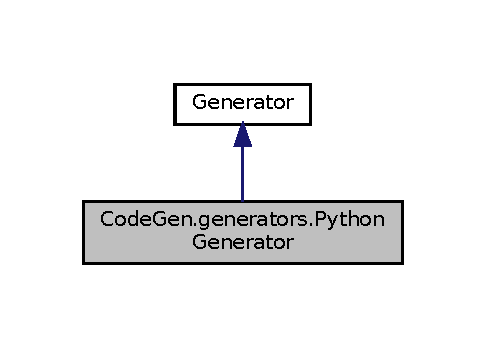
\includegraphics[width=233pt]{classCodeGen_1_1generators_1_1PythonGenerator__inherit__graph}
\end{center}
\end{figure}


Collaboration diagram for Code\+Gen.\+generators.\+Python\+Generator\+:
\nopagebreak
\begin{figure}[H]
\begin{center}
\leavevmode
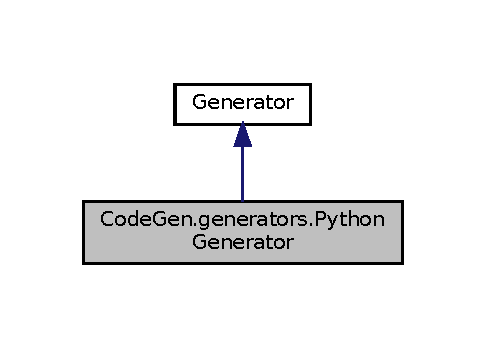
\includegraphics[width=233pt]{classCodeGen_1_1generators_1_1PythonGenerator__coll__graph}
\end{center}
\end{figure}
\subsection*{Protected Member Functions}
\begin{DoxyCompactItemize}
\item 
override string \mbox{\hyperlink{classCodeGen_1_1generators_1_1PythonGenerator_a7ef1629fdf50856e1424ed4fd8be564c}{Generate\+Class}} (\mbox{\hyperlink{classCodeGen_1_1generators_1_1Class}{Class}} @class)
\begin{DoxyCompactList}\small\item\em \mbox{\hyperlink{classCodeGen_1_1generators_1_1Class}{Class}} generator\+: generates class with fields, methods and subclasses from given class object  \end{DoxyCompactList}\item 
override string \mbox{\hyperlink{classCodeGen_1_1generators_1_1PythonGenerator_aafd171ffd14980515eef644b929bd712}{Generate\+Field}} (\mbox{\hyperlink{classCodeGen_1_1generators_1_1Field}{Field}} field)
\begin{DoxyCompactList}\small\item\em \mbox{\hyperlink{classCodeGen_1_1generators_1_1Field}{Field}} generator\+: generates field from given field object  \end{DoxyCompactList}\item 
override string \mbox{\hyperlink{classCodeGen_1_1generators_1_1PythonGenerator_a09ea61b8eb384efcc36aa3574f9cb6a8}{Generate\+Method}} (\mbox{\hyperlink{classCodeGen_1_1generators_1_1Method}{Method}} method)
\begin{DoxyCompactList}\small\item\em \mbox{\hyperlink{classCodeGen_1_1generators_1_1Method}{Method}} generator\+: generates method from given method object  \end{DoxyCompactList}\end{DoxyCompactItemize}
\subsection*{Additional Inherited Members}


\subsection{Detailed Description}
Python language generator 



\subsection{Member Function Documentation}
\mbox{\Hypertarget{classCodeGen_1_1generators_1_1PythonGenerator_a7ef1629fdf50856e1424ed4fd8be564c}\label{classCodeGen_1_1generators_1_1PythonGenerator_a7ef1629fdf50856e1424ed4fd8be564c}} 
\index{Code\+Gen\+::generators\+::\+Python\+Generator@{Code\+Gen\+::generators\+::\+Python\+Generator}!Generate\+Class@{Generate\+Class}}
\index{Generate\+Class@{Generate\+Class}!Code\+Gen\+::generators\+::\+Python\+Generator@{Code\+Gen\+::generators\+::\+Python\+Generator}}
\subsubsection{\texorpdfstring{Generate\+Class()}{GenerateClass()}}
{\footnotesize\ttfamily override string Code\+Gen.\+generators.\+Python\+Generator.\+Generate\+Class (\begin{DoxyParamCaption}\item[{\mbox{\hyperlink{classCodeGen_1_1generators_1_1Class}{Class}} @}]{class }\end{DoxyParamCaption})\hspace{0.3cm}{\ttfamily [inline]}, {\ttfamily [protected]}, {\ttfamily [virtual]}}



\mbox{\hyperlink{classCodeGen_1_1generators_1_1Class}{Class}} generator\+: generates class with fields, methods and subclasses from given class object  



Implements \mbox{\hyperlink{classCodeGen_1_1generators_1_1Generator_a8847fd8b6d408a0dfc087dcc1dc58340}{Code\+Gen.\+generators.\+Generator}}.

\mbox{\Hypertarget{classCodeGen_1_1generators_1_1PythonGenerator_aafd171ffd14980515eef644b929bd712}\label{classCodeGen_1_1generators_1_1PythonGenerator_aafd171ffd14980515eef644b929bd712}} 
\index{Code\+Gen\+::generators\+::\+Python\+Generator@{Code\+Gen\+::generators\+::\+Python\+Generator}!Generate\+Field@{Generate\+Field}}
\index{Generate\+Field@{Generate\+Field}!Code\+Gen\+::generators\+::\+Python\+Generator@{Code\+Gen\+::generators\+::\+Python\+Generator}}
\subsubsection{\texorpdfstring{Generate\+Field()}{GenerateField()}}
{\footnotesize\ttfamily override string Code\+Gen.\+generators.\+Python\+Generator.\+Generate\+Field (\begin{DoxyParamCaption}\item[{\mbox{\hyperlink{classCodeGen_1_1generators_1_1Field}{Field}}}]{field }\end{DoxyParamCaption})\hspace{0.3cm}{\ttfamily [inline]}, {\ttfamily [protected]}, {\ttfamily [virtual]}}



\mbox{\hyperlink{classCodeGen_1_1generators_1_1Field}{Field}} generator\+: generates field from given field object  



Implements \mbox{\hyperlink{classCodeGen_1_1generators_1_1Generator_a0d1a48aedbca08c05af734a43739d1c3}{Code\+Gen.\+generators.\+Generator}}.

\mbox{\Hypertarget{classCodeGen_1_1generators_1_1PythonGenerator_a09ea61b8eb384efcc36aa3574f9cb6a8}\label{classCodeGen_1_1generators_1_1PythonGenerator_a09ea61b8eb384efcc36aa3574f9cb6a8}} 
\index{Code\+Gen\+::generators\+::\+Python\+Generator@{Code\+Gen\+::generators\+::\+Python\+Generator}!Generate\+Method@{Generate\+Method}}
\index{Generate\+Method@{Generate\+Method}!Code\+Gen\+::generators\+::\+Python\+Generator@{Code\+Gen\+::generators\+::\+Python\+Generator}}
\subsubsection{\texorpdfstring{Generate\+Method()}{GenerateMethod()}}
{\footnotesize\ttfamily override string Code\+Gen.\+generators.\+Python\+Generator.\+Generate\+Method (\begin{DoxyParamCaption}\item[{\mbox{\hyperlink{classCodeGen_1_1generators_1_1Method}{Method}}}]{method }\end{DoxyParamCaption})\hspace{0.3cm}{\ttfamily [inline]}, {\ttfamily [protected]}, {\ttfamily [virtual]}}



\mbox{\hyperlink{classCodeGen_1_1generators_1_1Method}{Method}} generator\+: generates method from given method object  



Implements \mbox{\hyperlink{classCodeGen_1_1generators_1_1Generator_a04fc9bd217b3b8c3d5f7b1a3f92c79d3}{Code\+Gen.\+generators.\+Generator}}.



The documentation for this class was generated from the following file\+:\begin{DoxyCompactItemize}
\item 
generators/\mbox{\hyperlink{Python_8cs}{Python.\+cs}}\end{DoxyCompactItemize}

\hypertarget{classCodeGen_1_1generators_1_1RubyGenerator}{}\section{Code\+Gen.\+generators.\+Ruby\+Generator Class Reference}
\label{classCodeGen_1_1generators_1_1RubyGenerator}\index{Code\+Gen.\+generators.\+Ruby\+Generator@{Code\+Gen.\+generators.\+Ruby\+Generator}}


Ruby language generator  




Inheritance diagram for Code\+Gen.\+generators.\+Ruby\+Generator\+:
\nopagebreak
\begin{figure}[H]
\begin{center}
\leavevmode
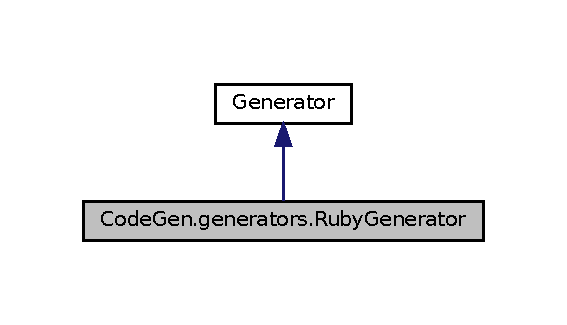
\includegraphics[width=272pt]{classCodeGen_1_1generators_1_1RubyGenerator__inherit__graph}
\end{center}
\end{figure}


Collaboration diagram for Code\+Gen.\+generators.\+Ruby\+Generator\+:
\nopagebreak
\begin{figure}[H]
\begin{center}
\leavevmode
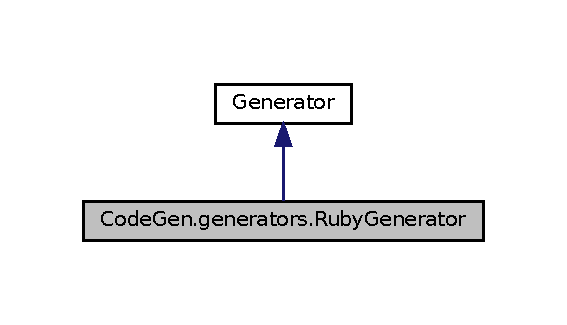
\includegraphics[width=272pt]{classCodeGen_1_1generators_1_1RubyGenerator__coll__graph}
\end{center}
\end{figure}
\subsection*{Protected Member Functions}
\begin{DoxyCompactItemize}
\item 
override string \mbox{\hyperlink{classCodeGen_1_1generators_1_1RubyGenerator_a5d54d68890f2fc6c58e297f79647c033}{Generate\+Class}} (\mbox{\hyperlink{classCodeGen_1_1generators_1_1Class}{Class}} @class)
\begin{DoxyCompactList}\small\item\em \mbox{\hyperlink{classCodeGen_1_1generators_1_1Class}{Class}} generator\+: generates class with fields, methods and subclasses from given class object  \end{DoxyCompactList}\item 
override string \mbox{\hyperlink{classCodeGen_1_1generators_1_1RubyGenerator_a08fbd6d88c129901aa159e3a9a706278}{Generate\+Field}} (\mbox{\hyperlink{classCodeGen_1_1generators_1_1Field}{Field}} field)
\begin{DoxyCompactList}\small\item\em \mbox{\hyperlink{classCodeGen_1_1generators_1_1Field}{Field}} generator\+: generates field from given field object  \end{DoxyCompactList}\item 
override string \mbox{\hyperlink{classCodeGen_1_1generators_1_1RubyGenerator_aa37c187dae8e400b050dcddba10d216b}{Generate\+Method}} (\mbox{\hyperlink{classCodeGen_1_1generators_1_1Method}{Method}} method)
\begin{DoxyCompactList}\small\item\em \mbox{\hyperlink{classCodeGen_1_1generators_1_1Method}{Method}} generator\+: generates method from given method object  \end{DoxyCompactList}\end{DoxyCompactItemize}
\subsection*{Additional Inherited Members}


\subsection{Detailed Description}
Ruby language generator 



\subsection{Member Function Documentation}
\mbox{\Hypertarget{classCodeGen_1_1generators_1_1RubyGenerator_a5d54d68890f2fc6c58e297f79647c033}\label{classCodeGen_1_1generators_1_1RubyGenerator_a5d54d68890f2fc6c58e297f79647c033}} 
\index{Code\+Gen\+::generators\+::\+Ruby\+Generator@{Code\+Gen\+::generators\+::\+Ruby\+Generator}!Generate\+Class@{Generate\+Class}}
\index{Generate\+Class@{Generate\+Class}!Code\+Gen\+::generators\+::\+Ruby\+Generator@{Code\+Gen\+::generators\+::\+Ruby\+Generator}}
\subsubsection{\texorpdfstring{Generate\+Class()}{GenerateClass()}}
{\footnotesize\ttfamily override string Code\+Gen.\+generators.\+Ruby\+Generator.\+Generate\+Class (\begin{DoxyParamCaption}\item[{\mbox{\hyperlink{classCodeGen_1_1generators_1_1Class}{Class}} @}]{class }\end{DoxyParamCaption})\hspace{0.3cm}{\ttfamily [inline]}, {\ttfamily [protected]}, {\ttfamily [virtual]}}



\mbox{\hyperlink{classCodeGen_1_1generators_1_1Class}{Class}} generator\+: generates class with fields, methods and subclasses from given class object  



Implements \mbox{\hyperlink{classCodeGen_1_1generators_1_1Generator_a8847fd8b6d408a0dfc087dcc1dc58340}{Code\+Gen.\+generators.\+Generator}}.

\mbox{\Hypertarget{classCodeGen_1_1generators_1_1RubyGenerator_a08fbd6d88c129901aa159e3a9a706278}\label{classCodeGen_1_1generators_1_1RubyGenerator_a08fbd6d88c129901aa159e3a9a706278}} 
\index{Code\+Gen\+::generators\+::\+Ruby\+Generator@{Code\+Gen\+::generators\+::\+Ruby\+Generator}!Generate\+Field@{Generate\+Field}}
\index{Generate\+Field@{Generate\+Field}!Code\+Gen\+::generators\+::\+Ruby\+Generator@{Code\+Gen\+::generators\+::\+Ruby\+Generator}}
\subsubsection{\texorpdfstring{Generate\+Field()}{GenerateField()}}
{\footnotesize\ttfamily override string Code\+Gen.\+generators.\+Ruby\+Generator.\+Generate\+Field (\begin{DoxyParamCaption}\item[{\mbox{\hyperlink{classCodeGen_1_1generators_1_1Field}{Field}}}]{field }\end{DoxyParamCaption})\hspace{0.3cm}{\ttfamily [inline]}, {\ttfamily [protected]}, {\ttfamily [virtual]}}



\mbox{\hyperlink{classCodeGen_1_1generators_1_1Field}{Field}} generator\+: generates field from given field object  



Implements \mbox{\hyperlink{classCodeGen_1_1generators_1_1Generator_a0d1a48aedbca08c05af734a43739d1c3}{Code\+Gen.\+generators.\+Generator}}.

\mbox{\Hypertarget{classCodeGen_1_1generators_1_1RubyGenerator_aa37c187dae8e400b050dcddba10d216b}\label{classCodeGen_1_1generators_1_1RubyGenerator_aa37c187dae8e400b050dcddba10d216b}} 
\index{Code\+Gen\+::generators\+::\+Ruby\+Generator@{Code\+Gen\+::generators\+::\+Ruby\+Generator}!Generate\+Method@{Generate\+Method}}
\index{Generate\+Method@{Generate\+Method}!Code\+Gen\+::generators\+::\+Ruby\+Generator@{Code\+Gen\+::generators\+::\+Ruby\+Generator}}
\subsubsection{\texorpdfstring{Generate\+Method()}{GenerateMethod()}}
{\footnotesize\ttfamily override string Code\+Gen.\+generators.\+Ruby\+Generator.\+Generate\+Method (\begin{DoxyParamCaption}\item[{\mbox{\hyperlink{classCodeGen_1_1generators_1_1Method}{Method}}}]{method }\end{DoxyParamCaption})\hspace{0.3cm}{\ttfamily [inline]}, {\ttfamily [protected]}, {\ttfamily [virtual]}}



\mbox{\hyperlink{classCodeGen_1_1generators_1_1Method}{Method}} generator\+: generates method from given method object  



Implements \mbox{\hyperlink{classCodeGen_1_1generators_1_1Generator_a04fc9bd217b3b8c3d5f7b1a3f92c79d3}{Code\+Gen.\+generators.\+Generator}}.



The documentation for this class was generated from the following file\+:\begin{DoxyCompactItemize}
\item 
generators/\mbox{\hyperlink{Ruby_8cs}{Ruby.\+cs}}\end{DoxyCompactItemize}

\hypertarget{classCodeGen_1_1utils_1_1Utils}{}\section{Code\+Gen.\+utils.\+Utils Class Reference}
\label{classCodeGen_1_1utils_1_1Utils}\index{Code\+Gen.\+utils.\+Utils@{Code\+Gen.\+utils.\+Utils}}


 




\subsection{Detailed Description}




The documentation for this class was generated from the following file\+:\begin{DoxyCompactItemize}
\item 
utils/\mbox{\hyperlink{Utils_8cs}{Utils.\+cs}}\end{DoxyCompactItemize}

\hypertarget{classCodeGen_1_1generators_1_1Variable}{}\section{Code\+Gen.\+generators.\+Variable Class Reference}
\label{classCodeGen_1_1generators_1_1Variable}\index{Code\+Gen.\+generators.\+Variable@{Code\+Gen.\+generators.\+Variable}}


The structure that describes variable. Contains name, type and default value  




Inheritance diagram for Code\+Gen.\+generators.\+Variable\+:
\nopagebreak
\begin{figure}[H]
\begin{center}
\leavevmode
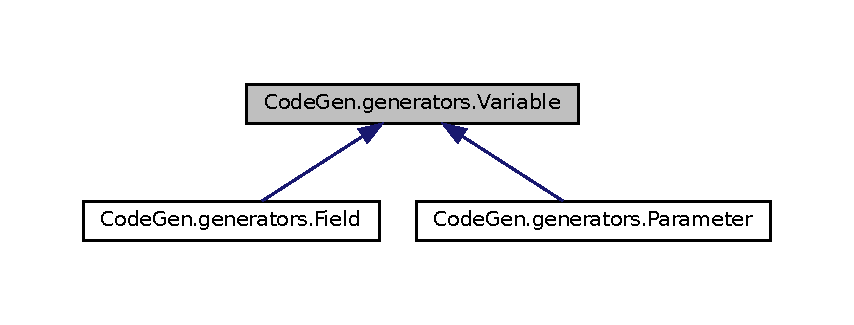
\includegraphics[width=350pt]{classCodeGen_1_1generators_1_1Variable__inherit__graph}
\end{center}
\end{figure}
\subsection*{Properties}
\begin{DoxyCompactItemize}
\item 
string \mbox{\hyperlink{classCodeGen_1_1generators_1_1Variable_a6b02f8bef23931e0a98adb0ff6399aed}{Name}}\hspace{0.3cm}{\ttfamily  \mbox{[}get, set\mbox{]}}
\begin{DoxyCompactList}\small\item\em Represents the name of the variable. Type\+: string \end{DoxyCompactList}\item 
string \mbox{\hyperlink{classCodeGen_1_1generators_1_1Variable_a42c04d2c0f45318b1fcf0fd8753bdbcf}{Type}}\hspace{0.3cm}{\ttfamily  \mbox{[}get, set\mbox{]}}
\begin{DoxyCompactList}\small\item\em Represents the type of the variable. Type\+: string \end{DoxyCompactList}\item 
string \mbox{\hyperlink{classCodeGen_1_1generators_1_1Variable_a773fcfe6f0e77f96ab75279c5f8c2051}{Default}}\hspace{0.3cm}{\ttfamily  \mbox{[}get, set\mbox{]}}
\begin{DoxyCompactList}\small\item\em Represents default value of the varibale. Type\+: string \end{DoxyCompactList}\end{DoxyCompactItemize}


\subsection{Detailed Description}
The structure that describes variable. Contains name, type and default value 



\subsection{Property Documentation}
\mbox{\Hypertarget{classCodeGen_1_1generators_1_1Variable_a773fcfe6f0e77f96ab75279c5f8c2051}\label{classCodeGen_1_1generators_1_1Variable_a773fcfe6f0e77f96ab75279c5f8c2051}} 
\index{Code\+Gen\+::generators\+::\+Variable@{Code\+Gen\+::generators\+::\+Variable}!Default@{Default}}
\index{Default@{Default}!Code\+Gen\+::generators\+::\+Variable@{Code\+Gen\+::generators\+::\+Variable}}
\subsubsection{\texorpdfstring{Default}{Default}}
{\footnotesize\ttfamily string Code\+Gen.\+generators.\+Variable.\+Default\hspace{0.3cm}{\ttfamily [get]}, {\ttfamily [set]}}



Represents default value of the varibale. Type\+: string 

\mbox{\Hypertarget{classCodeGen_1_1generators_1_1Variable_a6b02f8bef23931e0a98adb0ff6399aed}\label{classCodeGen_1_1generators_1_1Variable_a6b02f8bef23931e0a98adb0ff6399aed}} 
\index{Code\+Gen\+::generators\+::\+Variable@{Code\+Gen\+::generators\+::\+Variable}!Name@{Name}}
\index{Name@{Name}!Code\+Gen\+::generators\+::\+Variable@{Code\+Gen\+::generators\+::\+Variable}}
\subsubsection{\texorpdfstring{Name}{Name}}
{\footnotesize\ttfamily string Code\+Gen.\+generators.\+Variable.\+Name\hspace{0.3cm}{\ttfamily [get]}, {\ttfamily [set]}}



Represents the name of the variable. Type\+: string 

\mbox{\Hypertarget{classCodeGen_1_1generators_1_1Variable_a42c04d2c0f45318b1fcf0fd8753bdbcf}\label{classCodeGen_1_1generators_1_1Variable_a42c04d2c0f45318b1fcf0fd8753bdbcf}} 
\index{Code\+Gen\+::generators\+::\+Variable@{Code\+Gen\+::generators\+::\+Variable}!Type@{Type}}
\index{Type@{Type}!Code\+Gen\+::generators\+::\+Variable@{Code\+Gen\+::generators\+::\+Variable}}
\subsubsection{\texorpdfstring{Type}{Type}}
{\footnotesize\ttfamily string Code\+Gen.\+generators.\+Variable.\+Type\hspace{0.3cm}{\ttfamily [get]}, {\ttfamily [set]}}



Represents the type of the variable. Type\+: string 



The documentation for this class was generated from the following file\+:\begin{DoxyCompactItemize}
\item 
generators/\mbox{\hyperlink{Models_8cs}{Models.\+cs}}\end{DoxyCompactItemize}

\hypertarget{classCodeGen_1_1generators_1_1VbGenerator}{}\section{Code\+Gen.\+generators.\+Vb\+Generator Class Reference}
\label{classCodeGen_1_1generators_1_1VbGenerator}\index{Code\+Gen.\+generators.\+Vb\+Generator@{Code\+Gen.\+generators.\+Vb\+Generator}}


Visual Basic language generator  




Inheritance diagram for Code\+Gen.\+generators.\+Vb\+Generator\+:
\nopagebreak
\begin{figure}[H]
\begin{center}
\leavevmode
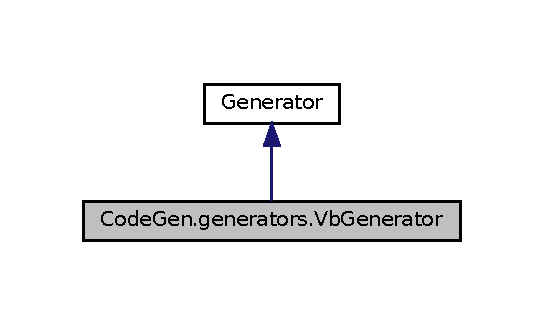
\includegraphics[width=261pt]{classCodeGen_1_1generators_1_1VbGenerator__inherit__graph}
\end{center}
\end{figure}


Collaboration diagram for Code\+Gen.\+generators.\+Vb\+Generator\+:
\nopagebreak
\begin{figure}[H]
\begin{center}
\leavevmode
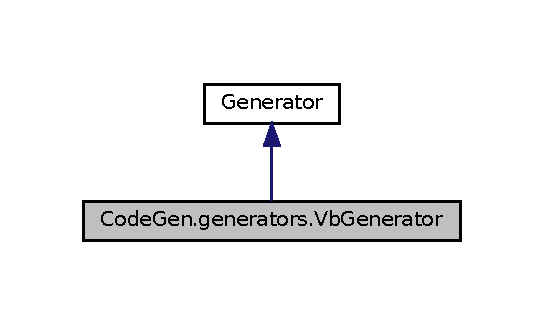
\includegraphics[width=261pt]{classCodeGen_1_1generators_1_1VbGenerator__coll__graph}
\end{center}
\end{figure}
\subsection*{Protected Member Functions}
\begin{DoxyCompactItemize}
\item 
override string \mbox{\hyperlink{classCodeGen_1_1generators_1_1VbGenerator_a78dd1bac9e915e214bb6a43b3ebc15b5}{Generate\+Class}} (\mbox{\hyperlink{classCodeGen_1_1generators_1_1Class}{Class}} @class)
\begin{DoxyCompactList}\small\item\em \mbox{\hyperlink{classCodeGen_1_1generators_1_1Class}{Class}} generator\+: generates class with fields, methods and subclasses from given class object  \end{DoxyCompactList}\item 
override string \mbox{\hyperlink{classCodeGen_1_1generators_1_1VbGenerator_a114f5fcd8cc13180701041b6d9815f3f}{Generate\+Field}} (\mbox{\hyperlink{classCodeGen_1_1generators_1_1Field}{Field}} field)
\begin{DoxyCompactList}\small\item\em \mbox{\hyperlink{classCodeGen_1_1generators_1_1Field}{Field}} generator\+: generates field from given field object  \end{DoxyCompactList}\item 
override string \mbox{\hyperlink{classCodeGen_1_1generators_1_1VbGenerator_ab8855feff4b8292c04a53362d270b34d}{Generate\+Method}} (\mbox{\hyperlink{classCodeGen_1_1generators_1_1Method}{Method}} method)
\begin{DoxyCompactList}\small\item\em \mbox{\hyperlink{classCodeGen_1_1generators_1_1Method}{Method}} generator\+: generates method from given method object  \end{DoxyCompactList}\end{DoxyCompactItemize}
\subsection*{Additional Inherited Members}


\subsection{Detailed Description}
Visual Basic language generator 



\subsection{Member Function Documentation}
\mbox{\Hypertarget{classCodeGen_1_1generators_1_1VbGenerator_a78dd1bac9e915e214bb6a43b3ebc15b5}\label{classCodeGen_1_1generators_1_1VbGenerator_a78dd1bac9e915e214bb6a43b3ebc15b5}} 
\index{Code\+Gen\+::generators\+::\+Vb\+Generator@{Code\+Gen\+::generators\+::\+Vb\+Generator}!Generate\+Class@{Generate\+Class}}
\index{Generate\+Class@{Generate\+Class}!Code\+Gen\+::generators\+::\+Vb\+Generator@{Code\+Gen\+::generators\+::\+Vb\+Generator}}
\subsubsection{\texorpdfstring{Generate\+Class()}{GenerateClass()}}
{\footnotesize\ttfamily override string Code\+Gen.\+generators.\+Vb\+Generator.\+Generate\+Class (\begin{DoxyParamCaption}\item[{\mbox{\hyperlink{classCodeGen_1_1generators_1_1Class}{Class}} @}]{class }\end{DoxyParamCaption})\hspace{0.3cm}{\ttfamily [inline]}, {\ttfamily [protected]}, {\ttfamily [virtual]}}



\mbox{\hyperlink{classCodeGen_1_1generators_1_1Class}{Class}} generator\+: generates class with fields, methods and subclasses from given class object  



Implements \mbox{\hyperlink{classCodeGen_1_1generators_1_1Generator_a8847fd8b6d408a0dfc087dcc1dc58340}{Code\+Gen.\+generators.\+Generator}}.

\mbox{\Hypertarget{classCodeGen_1_1generators_1_1VbGenerator_a114f5fcd8cc13180701041b6d9815f3f}\label{classCodeGen_1_1generators_1_1VbGenerator_a114f5fcd8cc13180701041b6d9815f3f}} 
\index{Code\+Gen\+::generators\+::\+Vb\+Generator@{Code\+Gen\+::generators\+::\+Vb\+Generator}!Generate\+Field@{Generate\+Field}}
\index{Generate\+Field@{Generate\+Field}!Code\+Gen\+::generators\+::\+Vb\+Generator@{Code\+Gen\+::generators\+::\+Vb\+Generator}}
\subsubsection{\texorpdfstring{Generate\+Field()}{GenerateField()}}
{\footnotesize\ttfamily override string Code\+Gen.\+generators.\+Vb\+Generator.\+Generate\+Field (\begin{DoxyParamCaption}\item[{\mbox{\hyperlink{classCodeGen_1_1generators_1_1Field}{Field}}}]{field }\end{DoxyParamCaption})\hspace{0.3cm}{\ttfamily [inline]}, {\ttfamily [protected]}, {\ttfamily [virtual]}}



\mbox{\hyperlink{classCodeGen_1_1generators_1_1Field}{Field}} generator\+: generates field from given field object  



Implements \mbox{\hyperlink{classCodeGen_1_1generators_1_1Generator_a0d1a48aedbca08c05af734a43739d1c3}{Code\+Gen.\+generators.\+Generator}}.

\mbox{\Hypertarget{classCodeGen_1_1generators_1_1VbGenerator_ab8855feff4b8292c04a53362d270b34d}\label{classCodeGen_1_1generators_1_1VbGenerator_ab8855feff4b8292c04a53362d270b34d}} 
\index{Code\+Gen\+::generators\+::\+Vb\+Generator@{Code\+Gen\+::generators\+::\+Vb\+Generator}!Generate\+Method@{Generate\+Method}}
\index{Generate\+Method@{Generate\+Method}!Code\+Gen\+::generators\+::\+Vb\+Generator@{Code\+Gen\+::generators\+::\+Vb\+Generator}}
\subsubsection{\texorpdfstring{Generate\+Method()}{GenerateMethod()}}
{\footnotesize\ttfamily override string Code\+Gen.\+generators.\+Vb\+Generator.\+Generate\+Method (\begin{DoxyParamCaption}\item[{\mbox{\hyperlink{classCodeGen_1_1generators_1_1Method}{Method}}}]{method }\end{DoxyParamCaption})\hspace{0.3cm}{\ttfamily [inline]}, {\ttfamily [protected]}, {\ttfamily [virtual]}}



\mbox{\hyperlink{classCodeGen_1_1generators_1_1Method}{Method}} generator\+: generates method from given method object  



Implements \mbox{\hyperlink{classCodeGen_1_1generators_1_1Generator_a04fc9bd217b3b8c3d5f7b1a3f92c79d3}{Code\+Gen.\+generators.\+Generator}}.



The documentation for this class was generated from the following file\+:\begin{DoxyCompactItemize}
\item 
generators/\mbox{\hyperlink{VB_8cs}{V\+B.\+cs}}\end{DoxyCompactItemize}

\chapter{File Documentation}
\hypertarget{Execute_8cs}{}\section{Execute.\+cs File Reference}
\label{Execute_8cs}\index{Execute.\+cs@{Execute.\+cs}}
\subsection*{Classes}
\begin{DoxyCompactItemize}
\item 
class {\bfseries Code\+Gen.\+Execute\+Conf}
\begin{DoxyCompactList}\small\item\em The configuration for execution, contains the application flow \end{DoxyCompactList}\end{DoxyCompactItemize}
\subsection*{Namespaces}
\begin{DoxyCompactItemize}
\item 
namespace \mbox{\hyperlink{namespaceCodeGen}{Code\+Gen}}
\end{DoxyCompactItemize}

\hypertarget{CSharp_8cs}{}\section{generators/\+C\+Sharp.cs File Reference}
\label{CSharp_8cs}\index{generators/\+C\+Sharp.\+cs@{generators/\+C\+Sharp.\+cs}}
\subsection*{Classes}
\begin{DoxyCompactItemize}
\item 
class \mbox{\hyperlink{classCodeGen_1_1generators_1_1CSharpGenerator}{Code\+Gen.\+generators.\+C\+Sharp\+Generator}}
\begin{DoxyCompactList}\small\item\em C\# language generator \end{DoxyCompactList}\end{DoxyCompactItemize}
\subsection*{Namespaces}
\begin{DoxyCompactItemize}
\item 
namespace \mbox{\hyperlink{namespaceCodeGen_1_1generators}{Code\+Gen.\+generators}}
\end{DoxyCompactItemize}

\hypertarget{ES6_8cs}{}\section{generators/\+E\+S6.cs File Reference}
\label{ES6_8cs}\index{generators/\+E\+S6.\+cs@{generators/\+E\+S6.\+cs}}
\subsection*{Classes}
\begin{DoxyCompactItemize}
\item 
class \mbox{\hyperlink{classCodeGen_1_1generators_1_1ES6Generator}{Code\+Gen.\+generators.\+E\+S6\+Generator}}
\begin{DoxyCompactList}\small\item\em \mbox{\hyperlink{classCodeGen_1_1generators_1_1Generator}{Generator}} for Java\+Script E\+S6 \end{DoxyCompactList}\end{DoxyCompactItemize}
\subsection*{Namespaces}
\begin{DoxyCompactItemize}
\item 
namespace \mbox{\hyperlink{namespaceCodeGen_1_1generators}{Code\+Gen.\+generators}}
\end{DoxyCompactItemize}

\hypertarget{GeneratorConf_8cs}{}\section{generators/\+Generator\+Conf.cs File Reference}
\label{GeneratorConf_8cs}\index{generators/\+Generator\+Conf.\+cs@{generators/\+Generator\+Conf.\+cs}}
\subsection*{Classes}
\begin{DoxyCompactItemize}
\item 
class \mbox{\hyperlink{classCodeGen_1_1generators_1_1Generator}{Code\+Gen.\+generators.\+Generator}}
\begin{DoxyCompactList}\small\item\em Interface of language generator \end{DoxyCompactList}\item 
class \mbox{\hyperlink{classCodeGen_1_1generators_1_1Normalizer}{Code\+Gen.\+generators.\+Normalizer}}
\begin{DoxyCompactList}\small\item\em Interface of language normalizer\+: normalizes package data according to specified language \end{DoxyCompactList}\item 
struct \mbox{\hyperlink{structCodeGen_1_1generators_1_1Languange}{Code\+Gen.\+generators.\+Languange}}
\begin{DoxyCompactList}\small\item\em The class that describes programming language and has a generator for it \end{DoxyCompactList}\item 
class \mbox{\hyperlink{classCodeGen_1_1generators_1_1GeneratorConf}{Code\+Gen.\+generators.\+Generator\+Conf}}
\begin{DoxyCompactList}\small\item\em Holds the configuration of generator \end{DoxyCompactList}\end{DoxyCompactItemize}
\subsection*{Namespaces}
\begin{DoxyCompactItemize}
\item 
namespace \mbox{\hyperlink{namespaceCodeGen_1_1generators}{Code\+Gen.\+generators}}
\end{DoxyCompactItemize}

\hypertarget{Go_8cs}{}\section{generators/\+Go.cs File Reference}
\label{Go_8cs}\index{generators/\+Go.\+cs@{generators/\+Go.\+cs}}
\subsection*{Classes}
\begin{DoxyCompactItemize}
\item 
class \mbox{\hyperlink{classCodeGen_1_1generators_1_1GoGenerator}{Code\+Gen.\+generators.\+Go\+Generator}}
\begin{DoxyCompactList}\small\item\em Go language generator \end{DoxyCompactList}\end{DoxyCompactItemize}
\subsection*{Namespaces}
\begin{DoxyCompactItemize}
\item 
namespace \mbox{\hyperlink{namespaceCodeGen_1_1generators}{Code\+Gen.\+generators}}
\end{DoxyCompactItemize}

\hypertarget{Groovy_8cs}{}\section{generators/\+Groovy.cs File Reference}
\label{Groovy_8cs}\index{generators/\+Groovy.\+cs@{generators/\+Groovy.\+cs}}
\subsection*{Classes}
\begin{DoxyCompactItemize}
\item 
class \mbox{\hyperlink{classCodeGen_1_1generators_1_1GroovyGenerator}{Code\+Gen.\+generators.\+Groovy\+Generator}}
\begin{DoxyCompactList}\small\item\em Groovy language generator \end{DoxyCompactList}\end{DoxyCompactItemize}
\subsection*{Namespaces}
\begin{DoxyCompactItemize}
\item 
namespace \mbox{\hyperlink{namespaceCodeGen_1_1generators}{Code\+Gen.\+generators}}
\end{DoxyCompactItemize}

\hypertarget{Java_8cs}{}\section{generators/\+Java.cs File Reference}
\label{Java_8cs}\index{generators/\+Java.\+cs@{generators/\+Java.\+cs}}
\subsection*{Classes}
\begin{DoxyCompactItemize}
\item 
class \mbox{\hyperlink{classCodeGen_1_1generators_1_1JavaGenerator}{Code\+Gen.\+generators.\+Java\+Generator}}
\begin{DoxyCompactList}\small\item\em Java language generator \end{DoxyCompactList}\end{DoxyCompactItemize}
\subsection*{Namespaces}
\begin{DoxyCompactItemize}
\item 
namespace \mbox{\hyperlink{namespaceCodeGen_1_1generators}{Code\+Gen.\+generators}}
\end{DoxyCompactItemize}

\hypertarget{Models_8cs}{}\section{generators/\+Models.cs File Reference}
\label{Models_8cs}\index{generators/\+Models.\+cs@{generators/\+Models.\+cs}}
\subsection*{Classes}
\begin{DoxyCompactItemize}
\item 
class \mbox{\hyperlink{classCodeGen_1_1generators_1_1Package}{Code\+Gen.\+generators.\+Package}}
\begin{DoxyCompactList}\small\item\em The structure that describes package. Contains classes and subpackages \end{DoxyCompactList}\item 
class \mbox{\hyperlink{classCodeGen_1_1generators_1_1Class}{Code\+Gen.\+generators.\+Class}}
\begin{DoxyCompactList}\small\item\em The structure that describes class. Contains name, array of fields, methods and subclasses, parent class name, access specifier. Overrides \mbox{\hyperlink{classCodeGen_1_1generators_1_1Class_a3d8c15ddeed8faad666f9dfdd53b758f}{To\+String()}} method. \end{DoxyCompactList}\item 
class \mbox{\hyperlink{classCodeGen_1_1generators_1_1Variable}{Code\+Gen.\+generators.\+Variable}}
\begin{DoxyCompactList}\small\item\em The structure that describes variable. Contains name, type and default value \end{DoxyCompactList}\item 
class \mbox{\hyperlink{classCodeGen_1_1generators_1_1Field}{Code\+Gen.\+generators.\+Field}}
\begin{DoxyCompactList}\small\item\em The structure that describes field. Contains access, const and static properties. Inherits from \mbox{\hyperlink{classCodeGen_1_1generators_1_1Variable}{Variable}} \end{DoxyCompactList}\item 
class \mbox{\hyperlink{classCodeGen_1_1generators_1_1Parameter}{Code\+Gen.\+generators.\+Parameter}}
\begin{DoxyCompactList}\small\item\em The structure that describes parameter. Inherits from \mbox{\hyperlink{classCodeGen_1_1generators_1_1Variable}{Variable}} \end{DoxyCompactList}\item 
class \mbox{\hyperlink{classCodeGen_1_1generators_1_1Method}{Code\+Gen.\+generators.\+Method}}
\begin{DoxyCompactList}\small\item\em The structure that describes method. Contains name, return type, access level, const and static properties and array of parameters \end{DoxyCompactList}\end{DoxyCompactItemize}
\subsection*{Namespaces}
\begin{DoxyCompactItemize}
\item 
namespace \mbox{\hyperlink{namespaceCodeGen_1_1generators}{Code\+Gen.\+generators}}
\end{DoxyCompactItemize}

\hypertarget{Python_8cs}{}\section{generators/\+Python.cs File Reference}
\label{Python_8cs}\index{generators/\+Python.\+cs@{generators/\+Python.\+cs}}
\subsection*{Classes}
\begin{DoxyCompactItemize}
\item 
class \mbox{\hyperlink{classCodeGen_1_1generators_1_1PythonGenerator}{Code\+Gen.\+generators.\+Python\+Generator}}
\begin{DoxyCompactList}\small\item\em Python language generator \end{DoxyCompactList}\end{DoxyCompactItemize}
\subsection*{Namespaces}
\begin{DoxyCompactItemize}
\item 
namespace \mbox{\hyperlink{namespaceCodeGen_1_1generators}{Code\+Gen.\+generators}}
\end{DoxyCompactItemize}

\hypertarget{Ruby_8cs}{}\section{generators/\+Ruby.cs File Reference}
\label{Ruby_8cs}\index{generators/\+Ruby.\+cs@{generators/\+Ruby.\+cs}}
\subsection*{Classes}
\begin{DoxyCompactItemize}
\item 
class \mbox{\hyperlink{classCodeGen_1_1generators_1_1RubyGenerator}{Code\+Gen.\+generators.\+Ruby\+Generator}}
\begin{DoxyCompactList}\small\item\em Ruby language generator \end{DoxyCompactList}\end{DoxyCompactItemize}
\subsection*{Namespaces}
\begin{DoxyCompactItemize}
\item 
namespace \mbox{\hyperlink{namespaceCodeGen_1_1generators}{Code\+Gen.\+generators}}
\end{DoxyCompactItemize}

\hypertarget{VB_8cs}{}\section{generators/\+VB.cs File Reference}
\label{VB_8cs}\index{generators/\+V\+B.\+cs@{generators/\+V\+B.\+cs}}
\subsection*{Classes}
\begin{DoxyCompactItemize}
\item 
class \mbox{\hyperlink{classCodeGen_1_1generators_1_1VbGenerator}{Code\+Gen.\+generators.\+Vb\+Generator}}
\begin{DoxyCompactList}\small\item\em Visual Basic language generator \end{DoxyCompactList}\item 
class {\bfseries Code\+Gen.\+generators.\+Vb\+Normalizer}
\end{DoxyCompactItemize}
\subsection*{Namespaces}
\begin{DoxyCompactItemize}
\item 
namespace \mbox{\hyperlink{namespaceCodeGen_1_1generators}{Code\+Gen.\+generators}}
\end{DoxyCompactItemize}

\hypertarget{Parser_8cs}{}\section{parser/\+Parser.cs File Reference}
\label{Parser_8cs}\index{parser/\+Parser.\+cs@{parser/\+Parser.\+cs}}
\subsection*{Classes}
\begin{DoxyCompactItemize}
\item 
class \mbox{\hyperlink{classCodeGen_1_1parser_1_1Parser}{Code\+Gen.\+parser.\+Parser}}
\begin{DoxyCompactList}\small\item\em \mbox{\hyperlink{classCodeGen_1_1parser_1_1Parser}{Parser}} \end{DoxyCompactList}\end{DoxyCompactItemize}
\subsection*{Namespaces}
\begin{DoxyCompactItemize}
\item 
namespace \mbox{\hyperlink{namespaceCodeGen_1_1parser}{Code\+Gen.\+parser}}
\end{DoxyCompactItemize}

\hypertarget{Program_8cs}{}\section{Program.\+cs File Reference}
\label{Program_8cs}\index{Program.\+cs@{Program.\+cs}}
\subsection*{Classes}
\begin{DoxyCompactItemize}
\item 
class {\bfseries Code\+Gen.\+Options}
\item 
class {\bfseries Code\+Gen.\+Program}
\end{DoxyCompactItemize}
\subsection*{Namespaces}
\begin{DoxyCompactItemize}
\item 
namespace \mbox{\hyperlink{namespaceCodeGen}{Code\+Gen}}
\end{DoxyCompactItemize}

\hypertarget{README_8md}{}\section{R\+E\+A\+D\+M\+E.\+md File Reference}
\label{README_8md}\index{R\+E\+A\+D\+M\+E.\+md@{R\+E\+A\+D\+M\+E.\+md}}

\hypertarget{GeneratorConfTest_8cs}{}\section{tests/generators/\+Generator\+Conf\+Test.cs File Reference}
\label{GeneratorConfTest_8cs}\index{tests/generators/\+Generator\+Conf\+Test.\+cs@{tests/generators/\+Generator\+Conf\+Test.\+cs}}
\subsection*{Classes}
\begin{DoxyCompactItemize}
\item 
class \mbox{\hyperlink{classCodeGen_1_1tests_1_1generators_1_1GeneratorConfTest}{Code\+Gen.\+tests.\+generators.\+Generator\+Conf\+Test}}
\end{DoxyCompactItemize}
\subsection*{Namespaces}
\begin{DoxyCompactItemize}
\item 
namespace \mbox{\hyperlink{namespaceCodeGen_1_1tests_1_1generators}{Code\+Gen.\+tests.\+generators}}
\end{DoxyCompactItemize}

\hypertarget{ParserTest_8cs}{}\section{tests/parser/\+Parser\+Test.cs File Reference}
\label{ParserTest_8cs}\index{tests/parser/\+Parser\+Test.\+cs@{tests/parser/\+Parser\+Test.\+cs}}
\subsection*{Classes}
\begin{DoxyCompactItemize}
\item 
class \mbox{\hyperlink{classCodeGen_1_1tests_1_1parser_1_1ParserTest}{Code\+Gen.\+tests.\+parser.\+Parser\+Test}}
\end{DoxyCompactItemize}
\subsection*{Namespaces}
\begin{DoxyCompactItemize}
\item 
namespace \mbox{\hyperlink{namespaceCodeGen_1_1tests_1_1parser}{Code\+Gen.\+tests.\+parser}}
\end{DoxyCompactItemize}

\hypertarget{Utils_8cs}{}\section{utils/\+Utils.cs File Reference}
\label{Utils_8cs}\index{utils/\+Utils.\+cs@{utils/\+Utils.\+cs}}
\subsection*{Classes}
\begin{DoxyCompactItemize}
\item 
class \mbox{\hyperlink{classCodeGen_1_1utils_1_1Utils}{Code\+Gen.\+utils.\+Utils}}
\end{DoxyCompactItemize}
\subsection*{Namespaces}
\begin{DoxyCompactItemize}
\item 
namespace \mbox{\hyperlink{namespaceCodeGen_1_1utils}{Code\+Gen.\+utils}}
\end{DoxyCompactItemize}

%--- End generated contents ---

% Index
\backmatter
\newpage
\phantomsection
\clearemptydoublepage
\addcontentsline{toc}{chapter}{Index}
\printindex

\end{document}
